\chapter{分类}
\label{chap:classification}

判断邮件是否为垃圾邮件，需要从预设类别中作出选择。\term{分类}（classification）从带标签样本学习这种决策。设$D_n=\{(\bm{x}_i,y_i)\}_{i=1}^{n}$，$\bm{x}_i\in\mathbb{R}^{d}$、$y_i\in\{1,\dots,C\}$，分类器为$f:\mathbb{R}^{d}\to\{1,\dots,C\}$；预测类别发生变化的位置构成\term{决策边界}（decision boundary）。本章讨论每个样本属于一个预设类别的单标签分类。

Fisher在1930年代用投影比较类间分离与类内波动，感知机在1950年代用错分反馈更新线性边界。1980年代的决策树将类别判断组织为递归条件测试；1990年代的支持向量机以间隔选择边界，并借助核内积表达非线性关系。树集成则组合多个成员的预测，把建树方式与成员间的误差关系纳入学习过程\scite{fisher1936,rosenblatt1958,cortes1995}。

在高维稀疏文本等任务中，线性分类器与朴素贝叶斯仍便于建立基线；在异质表格数据上，随机森林与梯度提升树是常用候选，需要与其他方法在相同预算下比较\scite{erickson2026tabarena}。本章按线性关系、邻域、树与规则、概率和集成展开：它们分别学习得分、聚合局部标签、使用条件分支、估计类别概率或组合成员；半监督分类随后说明怎样利用未标注样本。

除特别说明外，统计分析假设训练样本独立同分布，新样本独立来自同一分布。零一损失风险记为$R(f)=\mathbb{P}(f(\bm{x})\ne y)$，所有可测分类规则的最小风险记为$R^\ast$，即贝叶斯风险。模型类的可学习性比较的是算法风险与类内最低风险；候选类受限时，这个最低值可能高于$R^\ast$（二分类与有限多分类的学习条件分别参考\BookChapterRef{chap:binary-learnability}{第二卷“基础、理论和可信性”的“二分类学习的可学习性”章}与\BookChapterRef{chap:multiclass-learnability}{第二卷“基础、理论和可信性”的“多分类学习的可学习性”章}）。

\section{基于线性关系的分类}
\label{sec:classification-geometry}

线性得分用特征的加权和比较类别：把各项证据加权相加成一个分数，分数为正判一类、为负判另一类，决策边界因此是一条直线（高维中是超平面）。这种形式简单、易解释，但它本身没有回答一个关键问题：权重从哪里来？本节考察三种完全不同的确定权重的依据：LDA先描述每类数据的分布（类均值与协方差），再由统计量推出权重；感知机不假设分布，直接根据分类错误一次次修正权重；SVM既不估计分布也不被动纠错，而是主动在众多能分开数据的直线中选一条离两边都最远的。三种方法最后得到的得分形式几乎一样，学到的边界却可能很不同。核方法随后把内积换成特征空间内积，使相同的间隔准则能够表达非线性关系；线性表示的基础见第\ref{sec:classic-overview-linear}节。

LDA兼有投影与概率解释：这里推导共享协方差形式及其扩展，第\ref{sec:classification-probability}节再从类条件分布的角度联系这些协方差约束与高斯NB。Fisher准则评价投影后的类统计量，感知机的有限更新保证依赖正间隔可分性，软间隔SVM则在目标中允许间隔违反。三者的条件分别服务于投影、更新和优化，比较时需要保留各自的对象。

\subsection{线性判别分析（LDA）}
\label{sec:classification-lda}

用花瓣长度与宽度区分两类鸢尾花时，只比较两类平均长度可能会遗漏宽度提供的信息。把两项测量相加也未必合适：如果某项测量在同类花之间就有很大波动，它对区分类别的作用可能不及另一项；两项测量相关时，还要考虑它们是否重复提供了同一份信息。我们需要据此确定各特征的权重，并选择划分类别的阈值。

一种办法是先描述每类测量值围绕中心怎样变化，再比较新样本来自各类的可能性。\term{线性判别分析}（linear discriminant analysis, LDA）在高斯生成模型下采用这条路线：类均值给出中心，共享协方差刻画类内尺度与相关性，类先验记录类别比例。由这些量计算的后验概率，最终给出一个线性判别函数。协方差相同是这里的建模假设，并非所有分类数据都具有的性质。

LDA还有一个几何起点。Fisher在1936年的鸢尾花分类研究中寻找一种线性组合，使两类均值的差异相对于类内波动尽可能大。这一准则不要求样本服从高斯分布；它与高斯生成模型可以给出相同的判别方向，但概率解释和适用条件有所不同\scite{fisher1936}。

从两类的线性组合转向多个总体的判别，问题不再只是选择一条轴，还包括需要保留多少个方向。Rao在1948年系统讨论了多总体的生物分类与判别表示，这也为理解LDA如何从分类规则延伸为有监督降维方法提供了历史背景\scite{rao1948}。

\subsubsection{模型结构}
\label{sec:classification-lda-model}

沿用训练集$D_n=\{(\bm{x}_i,y_i)\}_{i=1}^{n}$，其中$\bm{x}_i\in\mathbb{R}^{d}$、$y_i\in\{1,\ldots,C\}$。生成式LDA假设
\begin{equation}
  \label{eq:classification-lda-distribution}
  \begin{aligned}
    \mathbb{P}(y=c)&=\pi_c,\qquad \pi_c>0,\quad
      \sum_{c=1}^{C}\pi_c=1,\\
    p(\bm{x}\mid y=c)&=\mathcal{N}(\bm{x};\bm{\mu}_c,\bm{\Sigma}),
      \qquad \bm{\Sigma}\succ0 .
  \end{aligned}
\end{equation}
这里$\bm{\mu}_c\in\mathbb{R}^{d}$描述第$c$类的中心，$\bm{\Sigma}\in\mathbb{R}^{d\times d}$描述类内各方向的波动及特征之间的相关性。共享协方差允许各类具有不同中心，同时规定中心附近相同的椭球形状和朝向；协方差中的非对角元仍可表示特征相关性。

在零一损失下，应选择后验概率最大的类别。取对数并展开高斯密度，有
\begin{equation}
  \label{eq:classification-lda-score}
  \begin{aligned}
    \log\{\pi_c p(\bm{x}\mid y=c)\}
      &=a(\bm{x})+\delta_c(\bm{x}),\\
    \delta_c(\bm{x})
      &=\bm{x}^{\top}\bm{\Sigma}^{-1}\bm{\mu}_c\\
      &\quad-\frac12\bm{\mu}_c^{\top}\bm{\Sigma}^{-1}\bm{\mu}_c
        +\log\pi_c .
  \end{aligned}
\end{equation}
其中$a(\bm{x})$收集了$-\bm{x}^{\top}\bm{\Sigma}^{-1}\bm{x}/2$、对数行列式和高斯归一化常数，均与类别无关。正是共享协方差使二次项在类别比较时抵消，留下关于$\bm{x}$的仿射函数。任意两类得分相等的位置通常为超平面；多分类的各类别区域由这些两两比较共同确定。

训练后把估计参数代入$\delta_c$，得到$\hat{\delta}_c$。预测规则及相应的模型后验为
\begin{equation}
  \label{eq:classification-lda-prediction}
  \begin{aligned}
    \hat f_{\mathrm{LDA}}(\bm{x})
      &=\argmax_{c\in\{1,\ldots,C\}}\hat{\delta}_c(\bm{x}),\\
    \hat p_c(\bm{x})
      &=\frac{\exp\{\hat{\delta}_c(\bm{x})\}}
        {\sum_{j=1}^{C}\exp\{\hat{\delta}_j(\bm{x})\}} .
  \end{aligned}
\end{equation}
本节对$\argmax$的平局统一选择索引最小的类别。共享协方差也限定了LDA能利用的类别差异。例如，设两类中心都在原点，一类的测量值集中在中心附近，另一类的测量值分散得更开。此时“离中心有多远”包含类别信息，但LDA中两类相同的均值使与输入有关的得分项完全相消，分类只能依据先验比例。若两类先验还相等，按真实均值形成的这组得分处处平局，固定类别的预测错误率为$1/2$。这说明该参数选择丢掉了尺度信息；整个LDA候选空间的限制将在表达能力分析中讨论。

让每类使用自己的$\bm{\Sigma}_c$，就能把这种尺度差异保留下来。这得到\term{二次判别分析}（quadratic discriminant analysis, QDA），即允许二次决策边界的高斯分类器\scite{hastie2009}。例如两类协方差分别为不同倍数的单位矩阵时，后验比较包含到原点的距离平方，可以形成围绕中心的球形边界。QDA同时需要为每类估计协方差；每类样本较少时，新增的参数也可能使估计更不稳定。

\subsubsection{参数学习}
\label{sec:classification-lda-learning}

\paragraph{生成模型的最大似然估计}
有标签样本已经给出了每个观测所属的高斯分量，因此这里不需要推断类别归属。令$n_c=\sum_{i=1}^{n}\mathbb{1}\{y_i=c\}$，暂设各类都有样本。忽略与参数无关的常数，对数似然为
\begin{equation}
  \label{eq:classification-lda-likelihood}
  \begin{aligned}
    \ell
      &=\sum_{c=1}^{C}n_c\log\pi_c
        -\frac n2\log\det\bm{\Sigma}\\
      &\quad-\frac12\sum_{c=1}^{C}\sum_{i:y_i=c}
        (\bm{x}_i-\bm{\mu}_c)^{\top}
        \bm{\Sigma}^{-1}(\bm{x}_i-\bm{\mu}_c).
  \end{aligned}
\end{equation}
对先验加入约束$\sum_c\pi_c=1$，拉格朗日驻点给出$n_c/\pi_c$为同一常数；归一化后该常数为$n$。对$\bm{\mu}_c$求导，则有$\bm{\Sigma}^{-1}\sum_{i:y_i=c}(\bm{x}_i-\bm{\mu}_c)=\bm{0}$。由此得到
\begin{equation}
  \label{eq:classification-lda-mean-prior}
  \hat\pi_c=\frac{n_c}{n},\qquad
  \hat{\bm{\mu}}_c=\frac1{n_c}\sum_{i:y_i=c}\bm{x}_i .
\end{equation}
这两个估计分别是类别出现频率和该类的样本均值。

把均值代回似然，定义\term{类内散度矩阵}（within-class scatter matrix）
\begin{equation}
  \label{eq:classification-lda-within}
  \bm{S}_{\mathrm{W}}
    =\sum_{c=1}^{C}\sum_{i:y_i=c}
      (\bm{x}_i-\hat{\bm{\mu}}_c)
      (\bm{x}_i-\hat{\bm{\mu}}_c)^{\top}.
\end{equation}
它累加每个样本相对于本类中心的偏离。用精度矩阵$\bm{\Omega}=\bm{\Sigma}^{-1}$改写剩余目标，得到$n\log\det\bm{\Omega}/2-\operatorname{tr}(\bm{\Omega}\bm{S}_{\mathrm{W}})/2$。其驻点满足$n\bm{\Omega}^{-1}=\bm{S}_{\mathrm{W}}$，故当$\bm{S}_{\mathrm{W}}\succ0$时，
\begin{equation}
  \label{eq:classification-lda-covariance}
  \hat{\bm{\Sigma}}=\frac1n\bm{S}_{\mathrm{W}} .
\end{equation}
对$\bm{\Omega}$的目标是严格凹的，因此该驻点给出最大似然解。

式~\eqref{eq:classification-lda-covariance}的分母是$n$，不是$n-C$。这种合并各类类内变动的估计称为\term{合并协方差}（pooled covariance），其无偏形式为
\[
  \hat{\bm{\Sigma}}_{\mathrm{U}}
    =\frac{\bm{S}_{\mathrm{W}}}{n-C},\qquad n>C .
\]
在共享协方差假设下，给定各类样本数，有$\mathbb{E}[\bm{S}_{\mathrm{W}}\mid y_1,\ldots,y_n]=(n-C)\bm{\Sigma}$，因为估计每个类中心各消耗一个自由度。最大似然与无偏估计是不同准则；两种估计渐近相同，但有限样本下有所区别。特别是先验不等时，整体缩放协方差会改变几何得分相对于$\log\hat\pi_c$的权重，预测边界未必相同。

闭式估计把训练归结为统计量累计和线性代数运算。稠密数据的类内散度累计需要$O(nd^2)$运算，矩阵分解需要$O(d^3)$运算。实现时分解一次$\hat{\bm{\Sigma}}$，再解$C$个线性方程组$\hat{\bm{\Sigma}}\bm{a}_c=\hat{\bm{\mu}}_c$；预存$\bm{a}_c$与常数项后，每个样本的预测成本为$O(Cd)$。这些计算要求协方差可逆。$\bm{S}_{\mathrm{W}}$奇异时，正定参数域内的最大似然解不存在，需用降维或正则化重新规定估计问题。

\paragraph{Fisher投影的学习}
生成模型之外，还可以直接比较投影后的类间分离与类内波动。令总样本均值$\hat{\bm{\mu}}=\sum_c(n_c/n)\hat{\bm{\mu}}_c$，定义\term{类间散度矩阵}（between-class scatter matrix）
\[
  \bm{S}_{\mathrm{B}}
    =\sum_{c=1}^{C}n_c
      (\hat{\bm{\mu}}_c-\hat{\bm{\mu}})
      (\hat{\bm{\mu}}_c-\hat{\bm{\mu}})^{\top}.
\]
它衡量各类中心相对于总中心的分散程度。投影到方向$\bm{w}$后，两种散度分别变为$\bm{w}^{\top}\bm{S}_{\mathrm{B}}\bm{w}$和$\bm{w}^{\top}\bm{S}_{\mathrm{W}}\bm{w}$。\term{Fisher判别准则}（Fisher discriminant criterion）取两者之比。以下假设$\bm{S}_{\mathrm{W}}\succ0$，使每个非零方向的分母都为正：
\begin{equation}
  \label{eq:classification-fisher-criterion}
  J(\bm{w})
    =\frac{\bm{w}^{\top}\bm{S}_{\mathrm{B}}\bm{w}}
      {\bm{w}^{\top}\bm{S}_{\mathrm{W}}\bm{w}},
    \qquad \bm{w}\ne\bm{0}.
\end{equation}
分子鼓励类中心远离，分母抑制同类样本投影后过于分散。

图~\ref{fig:classification-lda-projection}固定同一组二维教学样本，只改变单位投影方向。两类中心分别为$(-1,0)^{\top}$与$(1,0)^{\top}$，每类都加上偏移$(-0.3,-1)^{\top}$、$(-0.1,1)^{\top}$、$(0.1,1)^{\top}$、$(0.3,-1)^{\top}$。由这些点算得$\bm{S}_{\mathrm{W}}=\operatorname{diag}(2/5,8)$与$\bm{S}_{\mathrm{B}}=\operatorname{diag}(8,0)$，最优方向由$\bm{S}_{\mathrm{W}}^{-1}(\hat{\bm\mu}_2-\hat{\bm\mu}_1)$归一化得到$\bm w^\ast=(1,0)^{\top}$。它使投影均值相差$2$，合并类内方差为$0.05$；比较方向$\bm w_{\mathrm B}=(3/5,4/5)^{\top}$的均值间距为$1.2$、类内方差为$0.658$，所以两者的$J$分别为$20$与$180/329$。这里方差按总样本量$8$归一化；右侧浅色条只是样本投影的最小至最大范围，不能把它当作Fisher准则中的平方偏差。

\begin{figure}[htbp]
  \centering
  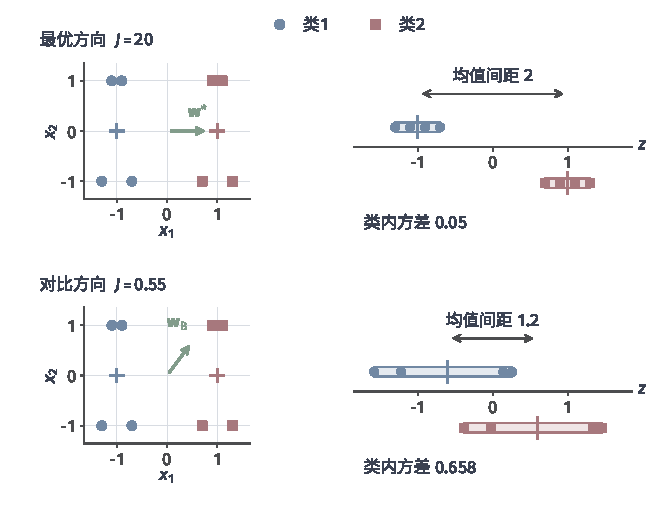
\includegraphics[width=112.000mm]{figures/04-classic-models/00-shared/matplotlib/classification-lda-target/figure.pdf}
  \caption{Fisher投影同时比较均值间距与类内散布。每类4个教学点，坐标无量纲；两行复用同一点集和相同投影数轴尺度。左侧绿色箭头为单位投影方向，十字为类均值；右侧短竖线为投影均值，浅色条为各类的样本投影范围，双向箭头标出均值间距。标注方差由$n^{-1}\bm w^{\top}\bm S_{\mathrm W}\bm w$计算，$J$仍按散度比计算。}
  \label{fig:classification-lda-projection}
\end{figure}

由于$J$不受$\bm{w}$的非零倍数缩放影响，可以约束$\bm{w}^{\top}\bm{S}_{\mathrm{W}}\bm{w}=1$。对$\bm{w}^{\top}\bm{S}_{\mathrm{B}}\bm{w}-\lambda(\bm{w}^{\top}\bm{S}_{\mathrm{W}}\bm{w}-1)$求导，得到\term{广义特征值问题}（generalized eigenvalue problem）：
\begin{equation}
  \label{eq:classification-fisher-eigenproblem}
  \bm{S}_{\mathrm{B}}\bm{w}
    =\lambda\bm{S}_{\mathrm{W}}\bm{w}.
\end{equation}
驻点还需比较大小。令$\bm{v}=\bm{S}_{\mathrm{W}}^{1/2}\bm{w}$，则
\[
  J(\bm{w})=\frac{\bm{v}^{\top}\bm{A}\bm{v}}{\bm{v}^{\top}\bm{v}},
  \qquad
  \bm{A}=\bm{S}_{\mathrm{W}}^{-1/2}
    \bm{S}_{\mathrm{B}}\bm{S}_{\mathrm{W}}^{-1/2}.
\]
把$\bm{v}$展开到对称半正定矩阵$\bm{A}$的正交特征向量上，上式就是各特征值的加权平均，权重非负且总和为$1$。最大值因而是最大特征值；取对应特征向量，再乘$\bm{S}_{\mathrm{W}}^{-1/2}$，便得到最优Fisher方向。若最大特征值有重数，最优方向未必唯一。

二分类时，令$\bm{h}=\hat{\bm{\mu}}_1-\hat{\bm{\mu}}_2\ne\bm{0}$，由总均值的定义可得
\[
  \bm{S}_{\mathrm{B}}=\frac{n_1n_2}{n}\bm{h}\bm{h}^{\top},
  \qquad
  \bm{w}_{\mathrm{F}}\propto\bm{S}_{\mathrm{W}}^{-1}\bm{h}.
\]
生成式LDA的法向量则为$\bm{w}_{\mathrm{G}}=\hat{\bm{\Sigma}}^{-1}\bm{h}=n\bm{S}_{\mathrm{W}}^{-1}\bm{h}$，两者方向相同。但完整的生成式分类规则还比较
\begin{equation}
  \label{eq:classification-lda-binary-threshold}
  \hat\delta_1(\bm{x})-\hat\delta_2(\bm{x})
    =\bm{w}_{\mathrm{G}}^{\top}
      \left(\bm{x}-\frac{\hat{\bm{\mu}}_1+\hat{\bm{\mu}}_2}{2}\right)
      +\log\frac{\hat\pi_1}{\hat\pi_2}
\end{equation}
的正负。Fisher准则本身只给方向，不给类先验、后验概率或这一阈值。两类均值相同时，均值散度准则没有正特征值方向，而生成模型仍可按先验选择类别。因此Fisher投影可用于非高斯数据，而贝叶斯最优性的证明还需要正确指定的高斯生成模型。

\subsubsection{理论分析}
\label{sec:classification-lda-analysis}

\paragraph{表达能力}
若真实类条件分布满足式\eqref{eq:classification-lda-distribution}，其后验概率就属于LDA的候选概率函数集，相应的贝叶斯决策也属于候选分类规则，无须用近似模型代替。共享协方差允许相关特征和不同类中心，但规定各类只有一个高斯峰，且峰周围的形状相同。即使不把得分解释为高斯后验，两个仿射得分的比较也只能产生一个半空间，不能表达任意形状的类别区域。

前面的同中心例子可以具体写成两类等先验、均值均为零，协方差分别为$\sigma_1^2\bm I_d$与$\sigma_2^2\bm I_d$，其中$0<\sigma_1<\sigma_2$。比较真实高斯密度得到：类1的贝叶斯区域是
\[
  \|\bm x\|_2^2<r_0^2,
  \qquad
  r_0^2=\frac{2d\log(\sigma_2/\sigma_1)}
                   {\sigma_1^{-2}-\sigma_2^{-2}}.
\]
小方差类在中心附近占优，大方差类在外侧占优。LDA的每个二类候选规则都以半空间作为类别区域，因而无法重现这个有界球。QDA保留半径平方项，候选空间能够表达这里的目标区域；两者的区别落在得分中是否允许这项二次关系。

\paragraph{收敛性}
固定训练集、各类别非空且类内散度正定时，生成式LDA的闭式参数达到该高斯模型的经验似然全局最大值，不需要迭代搜索。累积散度约需$O(nd^2)$运算，分解协方差约需$O(d^3)$运算；奇异情形没有这一正定域内的有限最优解。Fisher投影则通过广义特征值求解达到其比值准则的全局最大值，数值精度与矩阵条件数有关。

\paragraph{泛化性}
闭式估计只解决当前训练集上的拟合。下面先证明参数估计的\term{一致性}（consistency），再说明这些参数构成的分类器能否接近贝叶斯风险。给定训练集$D_n$后，$R(f\mid D_n)$只对独立新样本取平均。

\begin{lemma}[LDA参数估计的一致性]
  \label{thm:classification-lda-consistency}
  设$d$和$C$固定，训练样本独立同分布，真实分布满足式~\eqref{eq:classification-lda-distribution}，且所有$\pi_c^\ast>0$、$\bm{\Sigma}^\ast\succ0$。当$n\to\infty$时，
  \[
    \hat\pi_c\xrightarrow{\mathbb{P}}\pi_c^\ast,\qquad
    \hat{\bm{\mu}}_c\xrightarrow{\mathbb{P}}\bm{\mu}_c^\ast,\qquad
    \hat{\bm{\Sigma}}\xrightarrow{\mathbb{P}}\bm{\Sigma}^\ast .
  \]
  所有类别非空且$\hat{\bm{\Sigma}}$正定的概率趋于$1$。
\end{lemma}

\begin{proof}
  为处理随机的$n_c$，把类均值写成两个全样本平均之比：
  \[
    \hat{\bm{\mu}}_c
      =\frac{n^{-1}\sum_{i=1}^{n}\bm{x}_i\mathbb{1}\{y_i=c\}}
        {n^{-1}\sum_{i=1}^{n}\mathbb{1}\{y_i=c\}} .
  \]
  大数定律使分母收敛到$\pi_c^\ast>0$，分子收敛到$\pi_c^\ast\bm{\mu}_c^\ast$，因而先验和均值都一致。尚未观察到某一类时可以任意约定其均值；该事件的概率趋于零，不影响结论。

  共享协方差估计可展开为
  \[
    \hat{\bm{\Sigma}}
      =\frac1n\sum_{i=1}^{n}\bm{x}_i\bm{x}_i^{\top}
        -\sum_{c=1}^{C}\hat\pi_c
          \hat{\bm{\mu}}_c\hat{\bm{\mu}}_c^{\top}.
  \]
  高斯分布有有限二阶矩，故第一项收敛到
  \[
    \mathbb{E}[\bm{x}\bm{x}^{\top}]
      =\bm{\Sigma}^\ast+
        \sum_{c=1}^{C}\pi_c^\ast
          \bm{\mu}_c^\ast(\bm{\mu}_c^\ast)^{\top}.
  \]
  第二项消去类中心对二阶矩的贡献，余下$\bm{\Sigma}^\ast$。固定维数下，矩阵逐元素收敛也给出算子范数收敛；由$\bm{\Sigma}^\ast$的最小特征值严格为正，估计矩阵以趋于$1$的概率可逆。上述步骤实际上可由强大数定律加强为几乎必然收敛。
\end{proof}

矩阵求逆和$\log\pi_c$在这些条件下连续，所以在参数几乎必然收敛的事件上，对每个固定输入$\bm{x}$，有$\hat\delta_c(\bm{x})\to\delta_c^\ast(\bm{x})$。但$\argmax$在平局处不连续：在真实最大得分唯一的输入处，估计类别最终等于该输入的唯一贝叶斯类别；平局处则未必如此。若最优类别平局的输入集合概率为零，就能进一步推出随机输入上的预测标签收敛。不同贝叶斯分类器在平局处可以选择不同标签，却有相同风险。

参数收敛怎样传到预测错误率，可以直接通过类别后验比较，因而不需要排除后验平局。
\begin{theorem}[LDA在高斯同协方差条件下的期望分类风险界]
  \label{thm:classification-lda-risk}
  在引理\ref{thm:classification-lda-consistency}的条件下，用闭式估计的先验、均值和共享协方差构造$\hat p_c$，返回$\hat f_{\mathrm{LDA}}=\argmax_c\hat p_c$，平局按固定类别次序处理。不能拟合的训练集上暂用任意固定分类器。记真实后验为$p_c^\ast$，则在估计模型有定义时，
  \[
    0\leq R(\hat f_{\mathrm{LDA}}\mid D_n)-R^\ast
      \leq2\mathbb E_{\bm X}
        \max_c|\hat p_c(\bm X)-p_c^\ast(\bm X)|.
  \]
  随$n\to\infty$，左侧几乎必然趋于零，而且
  $\mathbb E_{D_n}R(\hat f_{\mathrm{LDA}}\mid D_n)\to R^\ast$。
\end{theorem}
\begin{proof}
记$f^\ast$为任意贝叶斯规则。由于$\hat f_{\mathrm{LDA}}$最大化$\hat p_c$，逐点有
\begin{equation}
  \label{eq:classification-lda-excess-risk}
  \begin{aligned}
    0&\leq p_{f^\ast(\bm{x})}^\ast(\bm{x})
      -p_{\hat f_{\mathrm{LDA}}(\bm{x})}^\ast(\bm{x})\\
      &\leq 2\max_{1\leq c\leq C}
          |\hat p_c(\bm{x})-p_c^\ast(\bm{x})| .
  \end{aligned}
\end{equation}
这个上界来自在两项之间分别加减相应的估计后验，并利用$\hat p_{\hat f_{\mathrm{LDA}}}\geq\hat p_{f^\ast}$。对独立测试输入积分，左侧成为超额风险，得到定理中的不等式。在参数几乎必然收敛的事件上，后验估计对每个输入收敛，右端的被积函数趋于零且不超过$2$；支配收敛定理给出条件风险的极限。再用风险位于$[0,1]$，对训练集取期望即可得到最后一个结论。由参数一致性引理，不能拟合的事件几乎必然最终不再出现。
\end{proof}

这条推理从训练统计量出发，经后验误差控制到独立新样本风险，依赖正确指定的高斯模型与固定维数。它给出风险极限，未给出有限样本速率；维数随样本量增长时也需另外分析。Fisher准则只评价投影的散度比例，没有这些分布条件时，不能由它推出上述风险结论。

\subsubsection{优化表达能力}

\paragraph{允许各类具有不同协方差}
\label{sec:classification-lda-covariance-extensions}
如果不同类别的类内变化方向和尺度明显不同，共享协方差就会限制LDA的表达能力。第\ref{sec:classification-lda-model}节已经定义的二次判别分析（QDA）保留类条件高斯假设，却为每个类别估计独立的协方差矩阵$\hat{\bm{\Sigma}}_c$。先假设各类协方差估计均正定，删去各类共同的常数项后，其判别得分为
\begin{equation}
  \begin{aligned}
    \delta_c(\bm{x})
      ={}&\log\hat{\pi}_c-\frac12\log\det\hat{\bm{\Sigma}}_c\\
        &-\frac12(\bm{x}-\hat{\bm{\mu}}_c)^\top
          \hat{\bm{\Sigma}}_c^{-1}(\bm{x}-\hat{\bm{\mu}}_c).
  \end{aligned}
  \label{eq:classification-qda-score}
\end{equation}
任意两类得分之差含有关于$\bm{x}$的二次项，所以边界一般是二次曲面。当协方差相同时，二次项相消，又得到 LDA。增加自由度也增加了估计负担：共享协方差模型需要$O(d^2+Cd)$个参数，QDA 则需要$O(Cd^2)$个参数；每一类只有少量样本时，独立协方差容易不稳定甚至奇异。第\ref{sec:classification-gda}节将从生成分布的角度统一这两种模型。

\paragraph{支持非线性关系}
\label{sec:classification-lda-kernel-extension}
QDA通过类协方差的差异产生二次边界；Fisher判别则可以从输入表示入手，改变只作线性投影的限制。例如，内外两圈样本在原坐标中的均值都可能接近原点，原坐标上的均值差便提供不了有用方向；增加距离平方等非线性特征后，两类在新坐标中可以具有不同均值。Mika等提出的\term{核 Fisher 判别}（kernel Fisher discriminant, KFD）在特征空间中重新计算类均值与散度，再最大化投影后的类间与类内散度比\scite{mika1999kernel}。
将投影方向写成$\bm{w}=\sum_{i=1}^n a_i\phi(\bm{x}_i)$，两种投影散度就都能写成系数$\bm{a}$与核矩阵构成的二次型，目标仍是它们的比值；类内散度的奇异性则用正则化处理。它与核 SVM 的区别仍在训练准则：KFD 关注整体类统计量，SVM 关注间隔及其违反程度。KFD 的基本解通常没有支持向量式的稀疏性，预测可能需要访问全部训练样本；若要从投影得分得到后验概率，还需额外建立得分分布或校准模型。
例如，内外两圈分别具有固定半径$1$与$2$时，径向特征$\phi(\bm x)=\|\bm x\|_2^2$把两类送到$1$与$4$。在二者之间设置阈值就能精确分开，带正则化的类内散度也不妨碍这个得分表示。若所选核仍只提供原坐标的线性组合，同中心两圈的均值差仍为零，Fisher准则便没有得到所需的径向信息。所选核是否保留径向信息，决定了这里的目标能否表达。

\subsubsection{优化泛化能力}

QDA放开了各类的形状，但少数类可能没有足够样本估计完整协方差。例如，一个类别只有10个样本，中心化后的样本协方差秩至多为9；若输入有20维，这个估计便无法求逆。完全改用LDA又会舍弃类间真实的尺度或方向差异。可以在两者之间折中，让各类借用一部分合并统计量。\term{正则化判别分析}（regularized discriminant analysis, RDA）通过收缩协方差控制这种取舍。Friedman的原始方法包含两个调节方向：将类内协方差向合并协方差收缩，再向球形协方差收缩\scite{friedman1989rda}。
记$n_c$为第$c$类样本数，$\hat{\bm{\Sigma}}$为以$n$为分母的合并协方差。一种与原始构造相符的写法是
\begin{equation}
  \begin{aligned}
    \bm{A}_c(a)
      &=\frac{(1-a)n_c\hat{\bm{\Sigma}}_c+an\hat{\bm{\Sigma}}}
              {(1-a)n_c+an},\\
    \tilde{\bm{\Sigma}}_c(a,b)
      &=(1-b)\bm{A}_c(a)
        +b\,\frac{\operatorname{tr}\bm{A}_c(a)}{d}\bm{I},
        \qquad a,b\in[0,1].
  \end{aligned}
  \label{eq:classification-rda}
\end{equation}
当$b=0$时，$a=0$与$a=1$分别对应 QDA 与 LDA 的协方差估计；增大$b$会减弱各方向方差差异，并在平均方差为正时帮助获得可逆估计。两个参数应在训练集内部通过验证选择。当合并协方差和各类协方差均奇异时，可逆性还需要平均方差为正的球形收缩项或其他正则化。

收缩也改变哪些类别差异能够进入得分。$a=1,b=0$时各类共享协方差，二次项相消；$b=1$时每类协方差都为单位矩阵的一个倍数，得分可以利用半径平方，却不能独立利用各方向的方差与特征相关性。只有保留完整的类特有协方差，才能表达前面QDA中的一般二次差异。RDA是在这些限制与估计波动之间选择，不是一个可以越过QDA分布族的新模型。

收缩强度越大，类形状越受限制；强度越小，越依赖每类样本估计完整协方差。应在训练数据内部选择强度，再检查独立数据上的分类误差与估计稳定性。

\subsubsection{小结}
\label{sec:classification-lda-summary}

LDA把类中心、类内波动与类别比例合成一个得分。共享协方差使两类比较中的二次项抵消，留下线性边界；高斯生成模型还给出后验与阈值。Fisher的投影准则则把均值分离和类内散布放在同一个比值中，适合解释各特征怎样参与判别，但只选方向，不能独自给出后验概率。

类形状不同时，QDA保留各类协方差，代价是每类都要有足够数据支持矩阵估计。小样本、高维条件下，Friedman的RDA让各类借用合并统计量，再按需要向球形协方差收缩，减轻独立估计的波动。收缩越强，能够保留的方向与尺度差异越少；收缩参数的选择也增加了验证工作。

另一类困难来自原坐标没有显示类别差异。内外两圈的均值可以相同，单纯调整协方差估计无法为线性Fisher投影补上径向关系。Mika等的核Fisher判别把类统计量移到特征空间，让非线性关系进入同一个散度准则。代价是核矩阵、散度正则化与通常较稠密的预测表示；核所保留的信息仍决定哪些目标能够表达。若任务需要多个判别方向，相关降维构造见第\ref{chap:dimensionality-reduction}章。

\subsection{感知机}
\label{sec:classification-perceptron}

LDA先估计每类分布，再由这些分布决定边界。若任务只要求给出类别，我们也可以直接用预测错误调整边界。例如，两类点虽然可以被一条直线分开，却沿不同方向伸展，不适合共享协方差的描述。寻找分隔线仍是有意义的任务，并不需要先把每类的分布拟合好。

\term{感知机}（perceptron）从一组初始权重出发，逐个检查训练样本；遇到分类条件被违反的样本，就沿提高其正确类别得分的方向修正权重。这样，标签直接告诉算法边界需要怎样移动。算法可在任意训练集上运行；若训练集具有正间隔可分性，才有后面证明的有限更新保证。Rosenblatt在1958年的论文中研究了这一学习机制，本节介绍其中广泛使用的线性阈值模型与误差修正规则\scite{rosenblatt1958}。

康奈尔航空实验室还用Mark I Perceptron将这一研究路线实现为电子装置。历史系统包含感觉、关联和响应等组织；本节抽取的是后来常用的单个线性分类器及其更新规则\scite{smithsonianMarkI}。

\subsubsection{模型结构}
\label{sec:classification-perceptron-model}

本小节先使用二分类标签$y_i\in\{-1,+1\}$。为了使偏置在更新规则和收敛证明中始终处于同一坐标系，引入\term{增广向量}（augmented vector），即在输入末尾补一个恒为$1$的分量，并把偏置并入参数：
\begin{equation}
  \label{eq:classification-perceptron-augmented}
  \tilde{\bm{x}}=
    \begin{pmatrix}\bm{x}\\1\end{pmatrix},\qquad
  \tilde{\bm{w}}=
    \begin{pmatrix}\bm{w}\\b\end{pmatrix}
    \in\mathbb{R}^{d+1}.
\end{equation}
其中$\bm{w}\in\mathbb{R}^{d}$，$b\in\mathbb{R}$。分类规则为
\begin{equation}
  \label{eq:classification-perceptron-prediction}
  f(\bm{x})=\operatorname{sign}
    (\tilde{\bm{w}}^{\top}\tilde{\bm{x}})
    =\operatorname{sign}(\bm{w}^{\top}\bm{x}+b).
\end{equation}
约定$\operatorname{sign}(s)=+1$当$s\geq0$，否则为$-1$。非退化边界$\bm{w}^{\top}\bm{x}+b=0$是在$d$维输入空间中的$(d-1)$维超平面。它与二分类LDA具有相同的边界形式；这里的参数来自错误反馈，输出是类别得分与标签，概率需要另建模型。

在这一表示下，正间隔可分是指存在单位向量$\bm{u}^\ast\in\mathbb{R}^{d+1}$和$\gamma>0$，使
\begin{equation}
  \label{eq:classification-perceptron-margin}
  \begin{aligned}
    y_i\langle\bm{u}^\ast,\tilde{\bm{x}}_i\rangle
      &\geq\gamma,\qquad i=1,\ldots,n,\\
    \|\bm{u}^\ast\|_2&=1,\qquad
    \|\tilde{\bm{x}}_i\|_2\leq R .
  \end{aligned}
\end{equation}
这里$R$约束的是增广输入，因此$R\geq\max_i\sqrt{\|\bm{x}_i\|_2^2+1}$。$\gamma$也是增广空间中的间隔；若$\bm{u}^\ast=(\bm{v}^{\top},a)^{\top}/\sqrt{\|\bm{v}\|_2^2+a^2}$，其分母包含偏置$a$，不同于原输入空间中以$\|\bm{v}\|_2$归一化的几何距离。有限训练集只要能被仿射超平面严格分开，就存在这样的正$\gamma$。

线性表示的边界也很具体。例如异或任务把$(0,0)$、$(1,1)$标为负类，把$(1,0)$、$(0,1)$标为正类。按上述平局规则，前两点要求$b<0$和$w_1+w_2+b<0$，后两点要求$w_1+b\geq0$和$w_2+b\geq0$。前两式相加与后两式相加，对同一个$w_1+w_2+2b$给出矛盾要求。Minsky与Papert在1969年的《Perceptrons》中系统研究了此类表示能力限制；改变输入特征或加入非线性隐藏层可以越过单个线性边界的限制，但那已经改变了模型族\scite{minsky1969}。

\subsubsection{参数学习}
\label{sec:classification-perceptron-learning}

从$\tilde{\bm{w}}^{(0)}=\bm{0}$出发，若当前样本满足$y_i\langle\tilde{\bm{w}}^{(t)},\tilde{\bm{x}}_i\rangle\leq0$，便进行一次更新：
\begin{equation}
  \label{eq:classification-perceptron-update}
  \tilde{\bm{w}}^{(t+1)}
    =\tilde{\bm{w}}^{(t)}+\eta y_i\tilde{\bm{x}}_i,
    \qquad \eta>0 .
\end{equation}
这里$t$只数实际更新，学习率$\eta$保持不变。拆开最后一个分量，就是$\bm{w}\leftarrow\bm{w}+\eta y_i\bm{x}_i$和$b\leftarrow b+\eta y_i$。同一个样本的有符号得分增加$\eta\|\tilde{\bm{x}}_i\|_2^2$，所以更新确实朝修正当前判断的方向移动；但它可能同时破坏其他样本的正确分类，因而需要反复遍历。零得分也触发更新，即使按平局规则恰好预测为正确的正类，仍要求它离开边界。

图~\ref{fig:classification-perceptron-update}把这一步写成具体数值。取当前参数$\bm w=(1,0)^{\top}$、$b=-1$，正类点$\bm x_i=(0.5,1)^{\top}$的得分为$-0.5$，触发更新。学习率为$0.5$时，权重变为$(1.25,0.5)^{\top}$，偏置变为$-0.5$，当前点的得分增加到$0.625$。图中边界因此同时改变位置和方向；判断是否继续更新，仍要逐个检查后续样本。

\begin{figure}[htbp]
  \centering
  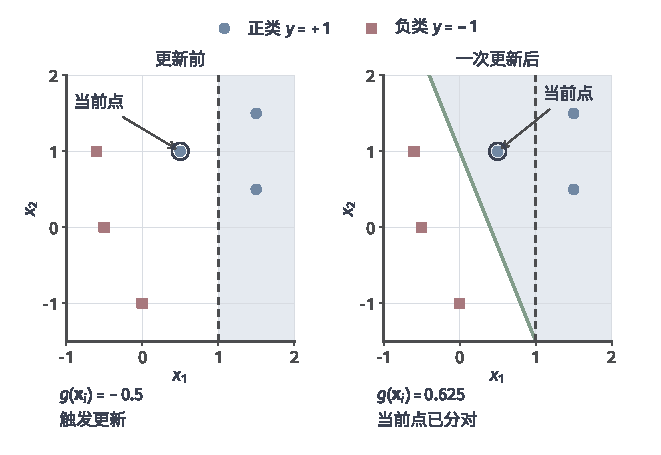
\includegraphics[width=112.000mm]{figures/04-classic-models/00-shared/matplotlib/classification-perceptron-update/figure.pdf}
  \caption{错分正类点触发的一次感知机更新。六个点为教学构造，坐标无量纲，两面板共用坐标范围；蓝圆、红方分别为正负类，黑色圆环标出当前点。浅蓝区域为正类预测区域，虚线为旧边界$x_1=1$，绿色实线为新边界$1.25x_1+0.5x_2=0.5$。偏置随权重一起更新，当前点由负得分变为正得分。}
  \label{fig:classification-perceptron-update}
\end{figure}

\begin{algorithm}[带遍历上限的感知机训练]
  \label{alg:classification-perceptron}
  \begin{algorithmic}[1]
    \Require $D_n$，固定学习率$\eta>0$，最大遍历轮数$E\geq1$
    \Ensure 参数$\tilde{\bm{w}}$与是否已验证收敛的状态
    \State $\tilde{\bm{w}}\gets\bm{0}$
    \For{$e=1,\ldots,E$}
      \State $m\gets0$
      \For{$i=1,\ldots,n$}
        \State $\tilde{\bm{x}}_i\gets(\bm{x}_i^{\top},1)^{\top}$
        \If{$y_i\langle\tilde{\bm{w}},\tilde{\bm{x}}_i\rangle\leq0$}
          \State $\tilde{\bm{w}}\gets\tilde{\bm{w}}+\eta y_i\tilde{\bm{x}}_i$
          \State $m\gets m+1$
        \EndIf
      \EndFor
      \If{$m=0$}
        \State \Return $(\tilde{\bm{w}},\text{已收敛})$
      \EndIf
    \EndFor
    \State \Return $(\tilde{\bm{w}},\text{达到轮数上限})$
  \end{algorithmic}
\end{algorithm}

一整轮没有更新时，所有样本都是在同一个参数下得到严格正的有符号得分，才构成收敛证据。达到轮数上限时返回的是预算内的当前解，可分性仍未由这一停止状态判定。稠密实现每轮需要$O(nd)$运算，除训练集外只需$O(d)$参数空间；样本访问顺序可以改变输出的分隔面。

从优化角度看，定义\term{感知机损失}（perceptron loss）
\begin{equation}
  \label{eq:classification-perceptron-loss}
  \ell_{\mathrm{P}}(\tilde{\bm{w}};\bm{x}_i,y_i)
    =\max\{0,-y_i\langle\tilde{\bm{w}},\tilde{\bm{x}}_i\rangle\}.
\end{equation}
为了把这项损失用于更新，先看它的两段：当带符号得分为负时，对参数求导得到$-y_i\tilde{\bm{x}}_i$；得分为正时，损失恒为零，梯度也是$\bm 0$。两段在零得分处相接，却给出不同斜率，普通梯度在这里没有定义。由于损失仍是凸的，可以使用次梯度；在交点处选择$-y_i\tilde{\bm{x}}_i$，仍满足支撑损失的仿射下界条件，也就得到式~\eqref{eq:classification-perceptron-update}。这一求解依据见\BookSectionRef{sec:opt-subgradient-methods}{第一卷“数学准备”的“基于次梯度的求解”节}。

上述更新逐样本执行；随机抽取样本时才相应成为随机次梯度下降。这里使用的是零间隔损失，不是标准的\term{合页损失}（hinge loss）$\max\{0,1-y_i\langle\tilde{\bm{w}},\tilde{\bm{x}}_i\rangle\}$。前者在零参数处就对所有样本取零，因此“感知机损失为零”本身不能证明分类正确；算法在零得分处仍更新的约定不可省略。

\subsubsection{理论分析}
\label{sec:classification-perceptron-analysis}

\paragraph{表达能力}
单层感知机的候选规则为$\operatorname{sign}(\bm w^\top\bm x+b)$。目标本来就是一个半空间时，这个候选类可以精确表示它；目标依赖特征交互时，则可能无法同时满足全部类别条件。

例如，取$(1,1)$、$(-1,-1)$、$(1,-1)$、$(-1,1)$四点作为输入域，同号坐标的目标标签为$-1$，异号坐标为$+1$。正、负两对点的中点都在原点。若一个仿射得分把四点全分对，正类得分的平均必须非负，负类得分的平均必须为负；两者却都等于$b$，产生矛盾。因此候选类中的每个函数至少在一个点上偏离目标。增加特征$x_1x_2$后，得分$-x_1x_2$恰好满足四点的目标标签，这才改变了候选空间的表示限制。

\paragraph{收敛性}
每次修正可能破坏已有判断，为什么这些修正不会无穷持续？关键是存在一个始终把所有样本分对的参考方向：更新朝该方向取得线性累积的进展，而参数范数的平方只能线性增长。Novikoff在1962年报告的证明清楚展示了这两个增长速度之间的矛盾\scite{novikoff1962}。

\begin{theorem}[感知机在有界可分样本下的最大更新次数]
  \label{thm:classification-perceptron-mistakes}
  若$D_n$满足式~\eqref{eq:classification-perceptron-margin}，从零参数出发，以固定$\eta>0$按式~\eqref{eq:classification-perceptron-update}更新，则对任意样本访问顺序，错误更新次数$M$满足
  \[
    M\leq\left(\frac R\gamma\right)^2 .
  \]
  这里错误更新包括零得分时的更新。若持续完整遍历训练集，且不因预算提前退出，算法在有限轮后得到所有训练样本上有符号得分均严格为正的参数。
\end{theorem}

\begin{proof}
  设第$t+1$次更新使用样本$i_t$。沿单位参考方向$\bm{u}^\ast$考察更新，得到
  \begin{align*}
    \langle\tilde{\bm{w}}^{(t+1)},\bm{u}^\ast\rangle
      &=\langle\tilde{\bm{w}}^{(t)},\bm{u}^\ast\rangle
        +\eta y_{i_t}\langle\tilde{\bm{x}}_{i_t},\bm{u}^\ast\rangle\\
      &\geq\langle\tilde{\bm{w}}^{(t)},\bm{u}^\ast\rangle+\eta\gamma .
  \end{align*}
  从零参数累加$M$次，便有
  \[
    \langle\tilde{\bm{w}}^{(M)},\bm{u}^\ast\rangle
      \geq M\eta\gamma .
  \]
  另一方面，展开更新后的平方范数：
  \begin{align*}
    \|\tilde{\bm{w}}^{(t+1)}\|_2^2
      &=\|\tilde{\bm{w}}^{(t)}\|_2^2
        +2\eta y_{i_t}
          \langle\tilde{\bm{w}}^{(t)},\tilde{\bm{x}}_{i_t}\rangle\\
      &\quad+\eta^2\|\tilde{\bm{x}}_{i_t}\|_2^2\\
      &\leq\|\tilde{\bm{w}}^{(t)}\|_2^2+\eta^2R^2 .
  \end{align*}
  不等式使用了更新条件：交叉项非正；并使用同一增广空间中的长度界$R$。再次累加，得到$\|\tilde{\bm{w}}^{(M)}\|_2^2\leq M\eta^2R^2$。由Cauchy--Schwarz不等式和$\|\bm{u}^\ast\|_2=1$，
  \[
    M\eta\gamma
      \leq\langle\tilde{\bm{w}}^{(M)},\bm{u}^\ast\rangle
      \leq\|\tilde{\bm{w}}^{(M)}\|_2
      \leq\eta R\sqrt{M}.
  \]
  $M=0$时结论直接成立；$M>0$时除以$\eta\sqrt M$再平方，得到所述界。因此更新不可能无限发生。持续完整遍历会在最后一次更新之后再检查所有样本；若仍有非正得分就还会更新，产生矛盾，故最终必有一整轮没有更新。
\end{proof}

这个界不显式含$n$，也不依赖访问顺序，但$R$和$\gamma$随数据而定；增加样本可能缩小可分间隔。它只约束更新次数，不包括寻找错误时检查正确样本的开销。对于算法~\ref{alg:classification-perceptron}的逐轮扫描，若不提前截断，至多需要$M+1$轮，包括最终的无更新确认轮。

若数据不可分，有限更新保证失效，持续遍历可能反复更新，此时可以限制训练预算并保留历史较好解，或采用允许间隔违约的在线方法。这些处理改变了停止或选解方式，仍须分别分析。

\paragraph{泛化性}
测试风险需要训练更新之外的统计条件。前述错误次数证明只考察给定样本的几何结构；若要判断未来预测，需要规定抽样分布与训练后返回哪个分类器。Cesa-Bianchi、Conconi与Gentile在2004年研究了这种联系：由独立同分布样本上的在线表现控制历史预测规则的风险，并讨论相应的输出选择方法\scite{cesabianchi2004generalization}。

下面给出一个期望风险的简单结论，说明额外条件怎样进入证明。按独立同分布的到达顺序，仅遍历$D_n$一次，从零参数出发使用固定学习率$\eta>0$和原更新规则。用$f_i$表示看到第$i$个样本之前的分类器；它只依赖$D_{i-1}$，其中$D_0$为空。这里$i$计数已访问的样本位置，与只计实际更新的$t$不同。训练后独立地从$\{1,\ldots,n\}$均匀抽取$I$，返回$f_I$，使输出规则与下述期望风险证明一致。

\begin{theorem}[感知机随机历史输出在可分分布下的期望风险界]
  \label{thm:classification-perceptron-risk}
  设训练样本独立同分布，测试样本独立来自同一分布。假设存在固定的单位向量$\bm{u}^\ast$及常数$R<\infty$、$\gamma>0$，使
  \[
    \|\tilde{\bm{x}}\|_2\leq R,\qquad
    y\langle\bm{u}^\ast,\tilde{\bm{x}}\rangle\geq\gamma
    \quad\text{几乎必然}.
  \]
  对上述单遍历训练和随机输出规则，有
  \begin{equation}
    \label{eq:classification-perceptron-risk}
    \mathbb{E}_{D_n,I}\!\left[R(f_I\mid D_n,I)\right]
      \leq\frac{R^2}{n\gamma^2}.
  \end{equation}
\end{theorem}

\begin{proof}
  令$e_i=\mathbb{1}\{f_i(\bm{x}_i)\ne y_i\}$。由于$f_i$尚未使用第$i$个样本，独立性给出
  \[
    \mathbb{E}[e_i\mid D_{i-1}]
      =R(f_i\mid D_{i-1}).
  \]
  对两边取期望，再对均匀的$I$平均，就有
  \[
    \mathbb{E}_{D_n,I}[R(f_I\mid D_n,I)]
      =\frac1n\sum_{i=1}^{n}\mathbb{E}[e_i].
  \]
  每次预测错误都会触发更新，零得分且预测正确时也可能更新，故$\sum_i e_i\leq M$。分布层面的共同间隔和长度界使定理~\ref{thm:classification-perceptron-mistakes}几乎必然适用于每个训练序列，于是$M\leq R^2/\gamma^2$，代入即得结论。
\end{proof}

这里的$R$和$\gamma$约束整个数据分布。式~\eqref{eq:classification-perceptron-risk}对训练抽样及随机历史状态取平均；当上界小于$1$时，它提供非平凡的期望风险控制。最终参数或多轮训练使用不同的输出与依赖关系，需各自分析：尤其在多轮中，当前样本已经参与既有参数的形成。不同的历史选解规则需要分别检查其训练依赖。

\subsubsection{优化表达能力}

若问题在于原空间不能线性分开，可把输入换成特征映射$\bm{\phi}(\bm{x})$。核函数$K(\bm{x},\bm{z})=\langle\bm{\phi}(\bm{x}),\bm{\phi}(\bm{z})\rangle$直接计算映射后的内积，省去显式构造高维坐标，得到\term{核感知机}（kernel perceptron）。为与前文偏置一致，使用增广映射$(\bm{\phi}(\bm{x}),1)$及其核$\tilde K(\bm{x},\bm{z})=K(\bm{x},\bm{z})+1$。零初始化、单位学习率下，参数在特征空间中是更新样本的线性组合，预测可写为
\begin{equation}
  \label{eq:classification-kernel-perceptron}
  f(\bm{x})=\operatorname{sign}
    \left(\sum_{i=1}^{n}\alpha_i y_i
      [K(\bm{x}_i,\bm{x})+1]\right).
\end{equation}
这里$\alpha_i$是样本$i$的更新次数；遇到非正有符号得分时令$\alpha_i\leftarrow\alpha_i+1$。必须选用正定核，即它在任意有限输入集上生成半正定Gram矩阵，才能作上述内积解释；有限更新还要求增广特征空间内存在正间隔，长度界相应变为$\sqrt{K(\bm{x}_i,\bm{x}_i)+1}$的上界。预测需要访问系数非零的样本，数量可能随训练增长。将内积推广到特征空间的思路可追溯至Aizerman、Braverman与Rozonoer在1964年的势函数研究\scite{aizerman1964}。

核与输入尺度共同决定映射后是否可分；预测成本则由需要保存的更新样本数决定。核化改变表示，不替代对标签噪声、停止规则和样本外误差的检查。

\subsubsection{优化泛化能力}

若希望减轻预测对最后一次参数更新的依赖，可以汇总训练过程中的多个状态。Freund与Schapire在1999年研究的\term{投票感知机}（voted perceptron）保存历次权重，并按各状态持续使用的次数加权投票；同一论文也比较了用历史得分平均代替投票的方式\scite{freund1999}。沿用本节的增广表示，设保存的状态为$\tilde{\bm w}_1,\ldots,\tilde{\bm w}_K$，$c_k>0$是第$k$个状态的计数，则投票预测为
\begin{equation}
  f_{\mathrm V}(\bm x)
  =\operatorname{sign}\!\left[
    \sum_{k=1}^{K}c_k\operatorname{sign}
       (\tilde{\bm w}_k^\top\tilde{\bm x})\right].
  \label{eq:classification-voted-perceptron}
\end{equation}
计数必须与更新同步。初始零参数的计数取零；本次检查未触发更新时，将当前状态的计数加一；触发更新时，保存新参数并把新状态的计数置为一，不再给被替换的旧状态加一。这里沿用非正有符号得分触发更新的约定，最后忽略计数为零的状态。计数取决于访问顺序与训练预算，并不是对新样本准确率的独立测量。保存与预测$K$个稠密状态均需考虑$O(Kd)$的代价。

\term{平均感知机}（averaged perceptron）改为先把这些增广参数平均：
\[
  \bar{\bm w}=\frac{\sum_{k=1}^{K}c_k\tilde{\bm w}_k}
                        {\sum_{k=1}^{K}c_k},
  \qquad
  f_{\mathrm A}(\bm x)=\operatorname{sign}
                    (\bar{\bm w}^\top\tilde{\bm x}).
\]
线性实现可在训练时累计参数和，最终只保存一组参数，额外存储与单次预测均为$O(d)$。投票先对每个得分取符号，再汇总标签；参数平均先汇总实值得分，再取符号，二者一般不同。前者的最终规则可以组合多个半空间判断，后者仍返回单个仿射得分；它们都改变训练结束后的输出方式，不能仅凭“汇总历史”判断哪种更适合任务。

\subsubsection{优化计算能力}

\paragraph{保存预算内的较优参数}
不可分数据可能使参数反复改变，预算结束时的权重未必是已经检查过的最好结果。\term{口袋算法}（Pocket algorithm）通过保存历史参数处理这个问题。常用版本额外保存$\tilde{\bm{w}}_{\mathrm{pocket}}$：每次检查候选参数时，计算全训练集零一错误数，仅在严格改进时替换记录；预算用尽后返回记录参数。它适用于噪声或矛盾标签数据，返回预算内已检查候选中的最小训练错误解；每次候选比较还需要评估全训练集。Gallant在1990年的论文中系统讨论了Pocket及相关学习方法\scite{gallant1990}。

Pocket只改变返回哪组历史参数，候选得分仍是原坐标中的仿射函数。它需要额外评估全部训练样本，也不能消除前面异或任务的表示限制。这里改善的是有限预算下的返回规则，并未使不可分数据上的原更新停止，也不保证找到所有仿射分类器中的最小训练错误解。

\paragraph{控制单步参数改动}
若希望每次更新不仅改正符号，还达到指定得分间隔，\term{被动攻击算法}（passive-aggressive algorithm, PA）把“尽量少改参数”和“满足当前样本的单位间隔”合成一个投影问题。用$\bm{v}$表示待求的新增广参数，
\begin{equation}
  \label{eq:classification-pa-projection}
  \begin{aligned}
    \min_{\bm{v}}\quad&
      \frac12\|\bm{v}-\tilde{\bm{w}}\|_2^2\\
    \text{满足}\quad&
      y_i\langle\bm{v},\tilde{\bm{x}}_i\rangle\geq1 .
  \end{aligned}
\end{equation}
令$\ell_i=\max\{0,1-y_i\langle\tilde{\bm{w}},\tilde{\bm{x}}_i\rangle\}$。约束已满足时参数不变；否则，拉格朗日驻点要求$\bm{v}=\tilde{\bm{w}}+\tau_i y_i\tilde{\bm{x}}_i$，将活跃约束代回即得
\[
  \tau_i=\frac{\ell_i}{\|\tilde{\bm{x}}_i\|_2^2},
  \qquad
  \tilde{\bm{w}}\leftarrow
    \tilde{\bm{w}}+\tau_i y_i\tilde{\bm{x}}_i .
\]
因此PA在间隔足够时“被动”，不足时按违约大小调整。增广方式也意味着这里把偏置变化纳入距离惩罚。噪声下硬性满足当前样本可能调整过大，PA-I可用$\tau_i=\min\{\lambda_{\mathrm{PA}},\ell_i/\|\tilde{\bm{x}}_i\|_2^2\}$限制步长，其中$\lambda_{\mathrm{PA}}>0$控制容忍程度。Crammer等人的2006年论文统一分析了这些在线大间隔方法；其保证针对在线更新的损失与间隔行为\scite{crammer2006}。
PA的单位间隔要求改变单步参数选择，候选得分仍是仿射函数。因此它与基本感知机、Pocket共享原坐标中的表示限制；间隔要求本身不能表达异或交互。

\subsubsection{支持多分类预测场景}

\label{sec:classification-perceptron-multiclass}

对$C$类问题，把标签改为$y_i\in\{1,\ldots,C\}$，每类维护一组增广参数$\tilde{\bm{w}}_c=(\bm{w}_c^{\top},b_c)^{\top}$，得分和预测为
\[
  s_c(\bm{x})=\langle\tilde{\bm{w}}_c,\tilde{\bm{x}}\rangle,
  \qquad
  \hat y=\argmax_{c\in\{1,\ldots,C\}}s_c(\bm{x}).
\]
平局仍按最小类别索引处理。这个构造把正确类别的得分与每个竞争类别作比较，也可用\term{Kesler构造}（Kesler construction）把这些比较写成一个扩展空间中的线性可分问题。

第$c$类获胜要求$s_c(\bm x)\geq s_j(\bm x)$对每个竞争类成立，平局处再按既定顺序处理。因此每类区域是若干半空间的交，仍是凸区域。它可以表示多类线性分区，却不能在原坐标中把某一类分成被其他类别隔开的多个区域；这种任务需要新的特征或不同的输出表示。

遇到$\hat y_i\ne y_i$时，只提高正确类别的参数并降低错误获胜类别的参数：
\begin{equation}
  \label{eq:classification-perceptron-multiclass-update}
  \begin{aligned}
    \tilde{\bm{w}}_{y_i}
      &\leftarrow\tilde{\bm{w}}_{y_i}+\eta\tilde{\bm{x}}_i,\\
    \tilde{\bm{w}}_{\hat y_i}
      &\leftarrow\tilde{\bm{w}}_{\hat y_i}-\eta\tilde{\bm{x}}_i .
  \end{aligned}
\end{equation}
其余类别不变，两个类别的偏置也随各自最后一个分量同时更新。若平局后预测错误，同样更新；若已选择正确类别，则该规则不更新。与二分类中所有零得分均更新的约定不同，这里直接按最终预测是否正确判断。

收敛条件也必须改为多类的得分差条件。把各类参数按行堆成$\tilde{\bm{W}}\in\mathbb{R}^{C\times(d+1)}$；假设存在$\|\bm{U}^\ast\|_{\mathrm{F}}=1$和$\gamma_{\mathrm{mc}}>0$，使对所有$i$和$c\ne y_i$都有
\[
  \langle\bm{U}_{y_i,:}^\ast-\bm{U}_{c,:}^\ast,
    \tilde{\bm{x}}_i\rangle\geq\gamma_{\mathrm{mc}} .
\]
这里$\|\cdot\|_{\mathrm{F}}$是所有矩阵元素平方和的平方根，行向量的内积按对应坐标计算。一次更新的方向矩阵仅两行非零，分别为$\tilde{\bm{x}}_i^{\top}$与$-\tilde{\bm{x}}_i^{\top}$，其平方范数至多为$2R^2$。它与$\bm{U}^\ast$的内积至少为$\gamma_{\mathrm{mc}}$；与当前参数的内积则为$s_{y_i}(\bm{x}_i)-s_{\hat y_i}(\bm{x}_i)\leq0$。因此零初始化时完全沿用二分类证明，得到
\[
  M\eta\gamma_{\mathrm{mc}}
    \leq\|\tilde{\bm{W}}^{(M)}\|_{\mathrm{F}}
    \leq\eta R\sqrt{2M},
  \qquad
  M\leq\frac{2R^2}{\gamma_{\mathrm{mc}}^2}.
\]
有限更新保证因而保留下来，但它要求所有正确类与竞争类之间都具有共同的正间隔，而不是只检查任意一对类别。

\subsubsection{支持结构化输出预测场景}

如果任务是给一句话中的每个词标注词性，输出就从一个类别变成了一整条标签序列。逐词独立判类无法在同一个得分中评价相邻标签的组合；我们希望同时比较不同候选序列，并在预测错误时调整整条序列用到的特征。\term{结构化感知机}（structured perceptron）把多分类的得分比较推广到结构之间，用联合特征$\bm{\phi}(\bm{x},y)$描述输入与候选结构，预测
\[
  \hat y_i=\argmax_{y\in Y(\bm{x}_i)}
    \langle\bm{\theta},\bm{\phi}(\bm{x}_i,y)\rangle ,
\]
其中$Y(\bm{x}_i)$是候选结构集合，$\bm{\theta}$是与联合特征同维的参数。解码错误时进行
\[
  \bm{\theta}\leftarrow\bm{\theta}
    +\eta\bigl[\bm{\phi}(\bm{x}_i,y_i)
      -\bm{\phi}(\bm{x}_i,\hat y_i)\bigr].
\]
联合特征决定哪些结构差异能够进入比较。若同一输入上的两个候选结构具有完全相同的$\bm\phi(\bm x,y)$，它们对所有参数都同分，候选得分无法区分两者，只能由固定的平局规则选择其中一个。词性标注中的相邻标签关系或更远处的依赖，因而需要由相应的特征记录；解码搜索再精确，也不能恢复特征没有保留的差异。

需要的类别或结构偏置也作为联合特征中的相应指示分量处理；对所有候选都相同的常数项会在得分差中消去。结构化输出增加了解码成本，近似解码还可能改变哪些样本触发更新，需要与特征设计一同评价。Collins在2002年将这种更新与参数平均用于序列标注，提供了词性标注和短语识别等实例，也为比较感知机与条件随机场等结构化模型提供了参照\scite{collins2002}。

\subsubsection{小结}
\label{sec:classification-perceptron-summary}

感知机用当前样本的标签直接修正边界，免去了先拟合类分布的步骤。一次更新提高当前样本的有符号得分，却可能改变其他样本的判断；因此样本顺序、停止预算和返回规则都属于实际学习过程。它提供简洁的增量训练方式，原坐标中的单个边界仍受仿射表示限制。

预算结束时怎样利用历史参数，是不可分或尚未收敛数据上的一个具体问题。Gallant讨论的Pocket保存已检查的较好状态，代价是重复评估训练集；Freund与Schapire的投票感知机让多个状态共同判类，代价是状态存储与多次预测。平均感知机把历史压缩成一组参数，减轻线性预测的负担，但它与标签投票采用不同的汇总规则。选择时需要比较同一访问顺序与预算下的分类误差和存储成本。

若缺的是非线性输入关系，核感知机把内积换到特征空间，预测则需要保留更新样本。PA处理的困难不同：当一步更新还不足以达到所需间隔时，Crammer等用最小参数改动满足当前约束，噪声下再限制过大的调整。它改变单步目标，原坐标中的表示仍然线性。

序列标注等结构化任务又需要改变输出比较。Collins的结构化感知机通过联合特征评价完整序列，解码成本随候选结构增加。输入表示、单步目标与输出结构解决不同困难，不能用增加遍历次数代替这些改变。

\subsection{支持向量机（SVM）}
\label{sec:classification-svm}

感知机回答了一个基本问题：如果训练样本能够被某个超平面分开，怎样通过错误驱动的更新找到一个分离器？但分开训练样本并不意味着分界的位置已经合适。同一批可分数据往往允许许多分离超平面，即使从零参数开始，感知机的结果仍会受样本顺序和更新规则影响。一个紧贴训练样本的边界虽然没有训练错误，却可能在输入受到很小扰动时改变预测。要在这些分离器之间作出选择，还需要说明什么样的边界更值得保留。

\term{支持向量机}（support vector machine，SVM）以训练样本到边界的距离选择分隔面：在正确分离样本的前提下，增大最近样本到边界的距离，称为最大间隔。给定特征表示与距离度量后，这个几何准则使边界具有可比较的尺度。不可分数据可以通过松弛约束处理，非线性关系则可以通过改变特征表示处理；两种扩展分别作用于误差容忍与候选函数。

核与松弛约束解决不同困难：Boser、Guyon与Vapnik在1992年把最大间隔训练与核表示结合，Cortes与Vapnik在1995年进一步系统发展了容许间隔违反的形式。前者改变非线性特征的使用方式，后者让噪声或类别重叠进入带惩罚的训练目标\scite{boser1992margin,cortes1995}。下面先从可分数据推导间隔目标与对偶，再用SMO说明参数怎样求出，最后分别改变输入表示、误差容忍和类别竞争。

\subsubsection{模型结构}
\label{sec:classification-svm-model}

沿用二分类标签约定，设训练集为$D_n=\{(\bm{x}_i,y_i)\}_{i=1}^n$，其中$\bm{x}_i\in\mathbb{R}^d$、$y_i\in\{-1,+1\}$，并假设两类均非空。令实值得分为$g(\bm{x})=\bm{w}^{\top}\bm{x}+b$，其中$\bm{w}\in\mathbb{R}^d$、$b\in\mathbb{R}$且$\bm{w}\ne\bm{0}$。决策超平面是$g(\bm{x})=0$，预测规则为$\hat y(\bm{x})=\operatorname{sign}(g(\bm{x}))$；若得分恰为零，约定预测为$+1$。

仅比较$y_i g(\bm{x}_i)$还不能比较不同超平面。把$(\bm{w},b)$同时乘以任意正数，分类结果不变，这个数值却会随之放大：同一条直线，把权重都乘以$100$，每个样本的得分也乘以$100$，直线却毫无变化。因此得分本身的“大小”带有任意性，不能直接当作距离或安全裕度。为区分参数尺度与真实距离，定义样本的\term{函数间隔}（functional margin）为$m_i=y_i g(\bm{x}_i)$，定义其\term{几何间隔}（geometric margin）为
\begin{equation}
  \gamma_i
  =\frac{y_i(\bm{w}^{\top}\bm{x}_i+b)}
         {\lVert\bm{w}\rVert_2},
  \qquad
  \gamma=\min_{1\le i\le n}\gamma_i.
  \label{eq:classification-svm-margin}
\end{equation}
函数间隔保留了得分的尺度；几何间隔除以法向量长度，得到沿法向方向测量的有符号距离。乘上真实标签后的得分满足$y_i g(\bm x_i)>0$时，样本位于正确类别一侧，这个距离为正。$g(\bm x_i)=0$时，样本就在决策边界上：正类虽然按平局规则被判对，几何间隔仍为零，因而没有正半径的扰动容忍保证。若输入改变为$\bm{x}_i+\bm{\Delta}$，由Cauchy--Schwarz不等式可得
\[
  y_i g(\bm{x}_i+\bm{\Delta})
  \ge y_i g(\bm{x}_i)
      -\lVert\bm{w}\rVert_2\lVert\bm{\Delta}\rVert_2.
\]
因此，$\lVert\bm{\Delta}\rVert_2<\gamma_i$时预测不会翻转。这说明间隔量化当前特征空间中、由该范数限定的输入扰动容忍程度；分布变化需要另外规定变化方式。

严格线性可分意味着存在$(\bm{w},b)$使所有$m_i>0$。由于样本数有限，可以将这组参数除以$\min_i m_i$，得到$\min_i m_i=1$的规范化表示。在该表示下，最近样本到决策超平面的单侧距离为$1/\lVert\bm{w}\rVert_2$；两个平行超平面$g(\bm{x})=+1$与$g(\bm{x})=-1$之间的总宽度则是$2/\lVert\bm{w}\rVert_2$。本节将前者记为$\gamma$，不把单侧间隔与两侧带宽混用。

最大化$\gamma$于是等价于最小化$\lVert\bm{w}\rVert_2$。平方与正比例因子不改变最优解，却使求导更方便，得到\term{硬间隔}（hard margin）SVM的原始问题：
\begin{equation}
  \begin{aligned}
    \min_{\bm{w},b}\quad&
      \frac12\lVert\bm{w}\rVert_2^2\\
    \text{s.t.}\quad&
      y_i(\bm{w}^{\top}\bm{x}_i+b)\ge1,
      \quad i=1,\ldots,n.
  \end{aligned}
  \label{eq:classification-svm-hard-primal}
\end{equation}
这里的“硬”表示每个样本都必须满足间隔约束，不能用其他样本的改善来补偿某个样本的违反。约束写为大于等于$1$并没有放弃规范化：若一个可行解的最小函数间隔严格大于$1$，将参数一起缩小就能降低目标，所以最优解必有紧约束。

可分时这个规范化问题有唯一解。先用一维点集观察间隔怎样选择边界，再推导求解所需的最优性条件。

\begin{example}[单侧间隔与带宽]
  \label{ex:classification-svm-one-dimensional}
  考虑一维教学数据$(x_1,y_1)=(-1,-1)$、$(x_2,y_2)=(1,+1)$、$(x_3,y_3)=(-2,-1)$和$(x_4,y_4)=(2,+1)$。任意落在$-1$与$1$之间的阈值都能正确分类，但只有阈值$0$使两侧最近距离的较小者达到最大。规范化最优解为$w^{\ast}=1$、$b^{\ast}=0$；最近样本的单侧距离为$1$，两条支持超平面在此退化为两个点$-1$与$1$，其间距离为$2$。更远的两个样本不限制这一最优间隔。
\end{example}

\subsubsection{参数学习}
\label{sec:classification-svm-learning}

每个间隔约束对最优边界的影响，可由对应的拉格朗日乘子表示。这里先用一句话说明“对偶”到底在做什么：原问题是在“选一条直线”，让它离样本尽量远；对偶则换一个视角，改问“每个训练样本对这条直线有多大约束力”。每个样本分到一个非负权重$\alpha_i$，离边界远、不构成约束的样本权重为零，真正“撑住”边界两侧的少数样本权重为正，它们就是后面的支持向量。\term{对偶问题}（dual problem）把这些约束权重作为优化变量，既揭示参与预测的样本，也把训练表示为样本间内积运算，为核化提供入口。原始与对偶的变量数分别受特征维数和样本数影响，计算选择还要结合求解器与数据稀疏性。

将约束写为$1-y_i(\bm{w}^{\top}\bm{x}_i+b)\le0$，引入$\alpha_i\ge0$，记$\bm{\alpha}=(\alpha_1,\ldots,\alpha_n)^{\top}$。拉格朗日函数为
\begin{equation}
  \begin{aligned}
    L(\bm{w},b,\bm{\alpha})
    ={}&\frac12\lVert\bm{w}\rVert_2^2\\
      &+\sum_{i=1}^n\alpha_i
        \bigl[1-y_i(\bm{w}^{\top}\bm{x}_i+b)\bigr].
  \end{aligned}
  \label{eq:classification-svm-hard-lagrangian}
\end{equation}
对一个可行$(\bm{w},b)$，$\sup_{\bm{\alpha}\ge\bm{0}}L$等于原始目标；若有约束违反，对应乘子趋于无穷会使上确界为正无穷。因此原始最优值可写为$\inf_{\bm{w},b}\sup_{\bm{\alpha}\ge\bm{0}}L$。反过来，先对$(\bm{w},b)$取下确界再最大化，得到原始最优值的下界。强对偶条件决定两种次序何时给出相同值。

这里可以直接核验\term{Slater条件}（Slater's condition）：它要求存在严格满足不等式约束的点。取一个严格分离器，并把参数放大到所有函数间隔都严格大于$1$，就得到所需点。结合目标凸、约束仿射以及定理\ref{thm:classification-svm-hard-unique}证明的最优值可达性，可得强对偶与最优乘子的存在性。

现在计算$q(\bm{\alpha})=\inf_{\bm{w},b}L(\bm{w},b,\bm{\alpha})$。由于$b$没有二次项，若$\sum_i\alpha_i y_i\ne0$，沿$b$的某个方向就有$L\to-\infty$。要使$q$有限，必须满足等式约束；关于$\bm{w}$的极小值则由驻点给出：
\begin{equation}
  \bm{w}=\sum_{i=1}^n\alpha_i y_i\bm{x}_i,
  \qquad
  \sum_{i=1}^n\alpha_i y_i=0.
  \label{eq:classification-svm-stationarity}
\end{equation}
令$\bm{v}=\sum_i\alpha_i y_i\bm{x}_i$，代入后涉及权重的两项变为$\frac12\lVert\bm{v}\rVert_2^2-\lVert\bm{v}\rVert_2^2$，而$b$项为零。展开$\lVert\bm{v}\rVert_2^2$，便得到
\begin{equation}
  \begin{aligned}
    \max_{\bm{\alpha}}\quad&
      q(\bm{\alpha})
      =\sum_{i=1}^n\alpha_i
       -\frac12\sum_{i,j=1}^n
          \alpha_i\alpha_j y_i y_j
          \bm{x}_i^{\top}\bm{x}_j\\
    \text{s.t.}\quad&
      \sum_{i=1}^n\alpha_i y_i=0,\qquad
      \alpha_i\ge0,\quad i=1,\ldots,n.
  \end{aligned}
  \label{eq:classification-svm-hard-dual}
\end{equation}
二次项矩阵的元素为$\bm{Q}_{i,j}=y_i y_j\bm{x}_i^{\top}\bm{x}_j$。对任意$\bm{a}\in\mathbb{R}^n$，有$\bm{a}^{\top}\bm{Q}\bm{a}=\lVert\sum_i a_i y_i\bm{x}_i\rVert_2^2\ge0$，所以$q$是凹函数；它未必严格凹，因而对偶乘子未必唯一。

原始解与对偶解的联系可以用\term{Karush--Kuhn--Tucker条件}（Karush--Kuhn--Tucker conditions，KKT条件）完整表达。它们同时检查解是否满足约束、是否达到驻点，以及一个约束是否真的限制了目标的继续改善。在当前凸问题与Slater条件下，这组条件对最优性既必要又充分：
\begin{equation}
  \begin{aligned}
    &m_i^{\ast}=y_i g^{\ast}(\bm{x}_i)\ge1,
      \qquad \alpha_i^{\ast}\ge0,\\
    &\alpha_i^{\ast}(m_i^{\ast}-1)=0,
      \qquad i=1,\ldots,n,\\
    &\bm{w}^{\ast}
      =\sum_{i=1}^n\alpha_i^{\ast}y_i\bm{x}_i,
      \qquad \sum_{i=1}^n\alpha_i^{\ast}y_i=0.
  \end{aligned}
  \label{eq:classification-svm-hard-kkt}
\end{equation}
其中第三个关系是\term{互补松弛}（complementary slackness）：乘子与约束的剩余量不能同时为正。最后一行是关于权重与偏置的驻点条件。

把$\alpha_i^{\ast}>0$的样本称为\term{支持向量}（support vector），并记其索引集为$S=\{i:\alpha_i^{\ast}>0\}$。互补松弛说明，支持向量一定满足$m_i^{\ast}=1$，而$m_i^{\ast}>1$必有$\alpha_i^{\ast}=0$。反向推断却不成立：落在边界上的样本也可能具有零乘子。例如把示例\ref{ex:classification-svm-one-dimensional}中的$x_2=1$重复一次，正类边界点的乘子总和仍可为$1/2$，但这个总量可以全部分配给其中一个副本。超平面没有改变，对偶表示与支持向量索引集却可能改变。

求得$\bm{\alpha}^{\ast}$后，恢复模型只需
\begin{equation}
  \begin{aligned}
    \bm{w}^{\ast}
      &=\sum_{i\in S}\alpha_i^{\ast}y_i\bm{x}_i,\\
    b^{\ast}
      &=y_k-(\bm{w}^{\ast})^{\top}\bm{x}_k,
        \qquad k\in S.
  \end{aligned}
  \label{eq:classification-svm-recover}
\end{equation}
精确最优解下，任意支持向量都会给出同一偏置；数值计算中可以平均多个合适样本给出的估计。只有非零乘子进入预测，这就是SVM的稀疏表示。表示的实际大小取决于支持向量数，某些训练集的大部分乃至全部样本都可能具有非零乘子。

\paragraph{SMO 算法}
\label{sec:classification-svm-smo}

对偶把未知量换成了$n$个乘子，也带来了新的计算负担。若存储完整内积矩阵，需要$O(n^2)$空间；通用稠密求解中的一次矩阵分解就可能需要$O(n^3)$运算，具体总成本还取决于求解器与迭代次数。为了避开每轮求解大规模二次规划，Platt提出了\term{序列最小优化}（sequential minimal optimization，SMO）：每次只优化一个最小的可动变量组，把整个问题分解为可解析处理的二维子问题\scite{platt1998smo}。

一次至少需要调整两个乘子，因为$\sum_i\alpha_i y_i=0$且$y_i\ne0$，单独改变一个$\alpha_i$会破坏等式约束。选择两个不同索引$i,j$，固定其余乘子，记更新前数值为$\alpha_i^{(t)},\alpha_j^{(t)}$，并令$s=y_i y_j\in\{-1,+1\}$。如果把新的$\alpha_j$写为$u$，等式约束要求
\begin{equation}
  \alpha_i(u)
  =\alpha_i^{(t)}
    +s\bigl(\alpha_j^{(t)}-u\bigr).
  \label{eq:classification-svm-smo-coupling}
\end{equation}
这样二维问题实际上只剩一个自由变量。对硬间隔，要求$u\ge0$且$\alpha_i(u)\ge0$，可行区间$[L,H]$为
\begin{equation}
  \begin{aligned}
    s=+1:\quad&
      L=0,\qquad H=\alpha_i^{(t)}+\alpha_j^{(t)},\\
    s=-1:\quad&
      L=\max\{0,\alpha_j^{(t)}-\alpha_i^{(t)}\},
      \qquad H=+\infty.
  \end{aligned}
  \label{eq:classification-svm-smo-hard-interval}
\end{equation}
同号时两乘子之和固定，因而有有限上界；异号时差固定，二者可以同时增大。这两种区间的差别来自标签符号对等式约束的影响。

为求沿这个区间的最优点，定义$\bm{K}_{i,j}=\bm{x}_i^{\top}\bm{x}_j$，并使用当前实值得分计算误差缓存
\[
  E_k=g^{(t)}(\bm{x}_k)-y_k,\qquad
  g^{(t)}(\bm{x})
  =\sum_{\ell=1}^n\alpha_\ell^{(t)}
     y_\ell\bm{x}_\ell^{\top}\bm{x}+b^{(t)}.
\]
$E_k$保留实值得分相对于标签的偏差，因而包含更新所需的距离信息；经过$\operatorname{sign}$得到的离散预测标签不再包含这部分信息。令$\Delta=u-\alpha_j^{(t)}$。由于$\Delta\alpha_i=-s\Delta$，权重变化为$y_j\Delta(\bm{x}_j-\bm{x}_i)$，代入$q$可以逐项得到
\begin{equation}
  \begin{aligned}
    q(u)-q(\alpha_j^{(t)})
      &=y_j(E_i-E_j)\Delta-\frac12\eta\Delta^2,\\
    \eta
      &=\bm{K}_{i,i}+\bm{K}_{j,j}-2\bm{K}_{i,j}\\
      &=\lVert\bm{x}_i-\bm{x}_j\rVert_2^2\ge0.
  \end{aligned}
  \label{eq:classification-svm-smo-gain}
\end{equation}
这里$q(u)$表示其余乘子固定、$\alpha_i$按式\eqref{eq:classification-svm-smo-coupling}联动后的目标。偏置不出现在对偶目标中；误差差$E_i-E_j$中的$b^{(t)}$也恰好相消。

当$\eta>0$时，一元凹二次函数的无约束最优点与区间最优点分别为
\begin{equation}
  \begin{aligned}
    u_{\mathrm{unc}}
      &=\alpha_j^{(t)}+\frac{y_j(E_i-E_j)}{\eta},\\
    \alpha_j^{(t+1)}
      &=\min\{H,\max\{L,u_{\mathrm{unc}}\}\},\\
    \alpha_i^{(t+1)}
      &=\alpha_i^{(t)}
        +s\bigl(\alpha_j^{(t)}-\alpha_j^{(t+1)}\bigr).
  \end{aligned}
  \label{eq:classification-svm-smo-update}
\end{equation}
剪裁只对一个自由变量进行，再由等式回代另一个；独立剪裁两个乘子会破坏耦合约束。若$L=H$，该变量对没有可行移动，应另选工作集。

$\eta=0$时，式\eqref{eq:classification-svm-smo-gain}变为线性函数，在有限区间上比较两个端点的目标即可；若目标恒定，保留旧值避免无效移动。严格可分的线性硬间隔问题中，$\eta=0$意味着两输入重合，它们不可能异号；同号重复点的目标沿可行线恒定。若出现零曲率、无穷上界且目标沿该方向无限增加，则应检查可分性假设、核矩阵与数值误差，并停止该次更新。

乘子更新以后还要调整偏置。记$\Delta\alpha_i=\alpha_i^{(t+1)}-\alpha_i^{(t)}$，$\Delta\alpha_j$同理。分别要求更新后的第$i$或第$j$个样本具有函数间隔$1$，解得
\begin{equation}
  \begin{aligned}
    b_i={}&b^{(t)}-E_i
       -y_i\Delta\alpha_i\bm{K}_{i,i}
       -y_j\Delta\alpha_j\bm{K}_{i,j},\\
    b_j={}&b^{(t)}-E_j
       -y_i\Delta\alpha_i\bm{K}_{i,j}
       -y_j\Delta\alpha_j\bm{K}_{j,j}.
  \end{aligned}
  \label{eq:classification-svm-smo-bias}
\end{equation}
硬间隔中，若更新后的$\alpha_i>0$，使用$b_i$；否则若$\alpha_j>0$，使用$b_j$。二者都为正且子问题精确求解时，这两个值一致；若都不能用于确定偏置，可暂取$(b_i+b_j)/2$。这一步利用当前工作集的条件更新偏置，其他样本是否满足KKT仍由后续全局扫描检查。

令$\Delta b=b^{(t+1)}-b^{(t)}$，其他样本的缓存可由
\[
  E_k^{(t+1)}
  =E_k^{(t)}
   +y_i\Delta\alpha_i\bm{K}_{i,k}
   +y_j\Delta\alpha_j\bm{K}_{j,k}
   +\Delta b
\]
更新，不必重新计算整个预测和。在示例\ref{ex:classification-svm-one-dimensional}中，从$\bm{\alpha}^{(0)}=\bm{0}$、$b^{(0)}=0$开始，选择$x_1=-1$与$x_2=1$，有$E_1=1$、$E_2=-1$、$\eta=4$，于是得到$\alpha_1=\alpha_2=1/2$和$b=0$。此时$w=1$，其余两个样本已经在间隔外；这一教学例子的最优解恰好由一次工作集更新达到；一般训练的迭代次数由后续选点与KKT误差决定。

\begin{algorithm}[硬间隔SMO的训练框架]
  \label{alg:classification-svm-smo}
  \begin{algorithmic}[1]
    \Require 两类非空且严格可分的$D_n$，容差$\varepsilon_{\mathrm{opt}}>0$，迭代上限$t_{\max}$
    \Ensure 可行乘子、偏置及停止状态
    \State 初始化$\bm{\alpha}^{(0)}=\bm{0}$、$b^{(0)}=0$、$E_k=-y_k$
    \For{$t=0,\ldots,t_{\max}-1$}
      \State 扫描KKT残差；若全部低于容差，返回“容差满足”
      \State 选取违反KKT的索引$i$，再选有可行改进的$j$
      \State 按式\eqref{eq:classification-svm-smo-hard-interval}计算$L,H$
      \State 求解一元子问题；退化时比较端点或更换变量对
      \State 联动更新两个乘子，更新$b$与误差缓存
    \EndFor
    \State 返回当前参数及“达到迭代上限，尚未认证收敛”
  \end{algorithmic}
\end{algorithm}

对于硬间隔，$\alpha_i=0$时应检查$m_i\ge1$，$\alpha_i>0$时应检查$m_i=1$，实际实现还要给“零乘子”设置数值容差。第二个变量可以优先选择误差差较大或预测目标增益较大的样本，并通过回退扫描持续检查其余违反条件的变量。算法\ref{alg:classification-svm-smo}给出共同框架，具体选点规则仍须保证持续处理违反KKT的变量。

SMO避免每轮分解整个稠密二次规划矩阵，但核缓存与工作集扫描仍有成本。

在线性问题中，也可以直接维护$\bm{w}$，不必先存储全部样本内积。软间隔形式还要处理合页损失：带符号得分跨过$1$时，损失从线性下降转为恒零，交点处没有普通梯度。次梯度方法允许在这个交点选择一个满足凸下界条件的方向，因而能继续更新参数。也可以按相应目标选择坐标下降算法。LIBLINEAR面向大规模稀疏线性分类提供了专门求解路线\scite{fan2008liblinear}。

\paragraph{最优解与停止证据}
\label{sec:classification-svm-analysis}
\label{sec:classification-svm-convergence}
\begin{theorem}[可分硬间隔问题的最优解]
  \label{thm:classification-svm-hard-unique}
  有限训练集严格线性可分、且两类均非空时，式\eqref{eq:classification-svm-hard-primal}存在唯一的规范化最优参数$(\bm w^\ast,b^\ast)$。
\end{theorem}
\begin{proof}
取一个可行解并限制目标不超过其值，权重便有界；一正一负两个样本的约束又给出偏置的上下界。因此可在非空紧水平集上取得最优值。平方范数对权重严格凸，所以不同最优解不能具有不同权重。

固定最优权重后，记正类投影最小值为$a_+$、负类投影最大值为$a_-$。可行偏置区间为$[1-a_+,-1-a_-]$，故$a_+-a_-\geq2$。若严格大于2，将权重和中心化偏置一起缩放到投影间距等于2，可保留全部约束却减小范数，违背最优性。故间距恰为2，偏置区间只剩一个点。
\end{proof}

SMO精确求解一个工作集时不会降低对偶目标，但目标单调不等于有限次到达全局最优。还要持续检查并处理所有违反KKT的变量，不能反复选择无法移动的变量对。实际训练以KKT容差给出近似最优证据；迭代预算先耗尽时，应保留“尚未达到容差”的状态。具体工作集规则及其收敛条件可参考分解算法研究\scite{osuna1997training,keerthi2002convergence,fan2005working}。

最大间隔是在固定表示和距离尺度下选择边界，不能单独保证新样本错误更少。线性SVM仍只能表示仿射分界；软化约束不会给它加入异或所需的交互特征。特征尺度、核与惩罚需要在训练集内部选择，最终用独立数据评价。下面把这几种改变分别写进得分和训练目标。

\subsubsection{核SVM与软间隔}

\paragraph{表示非线性分界}

\label{sec:classification-svm-kernels}

原坐标中的仿射得分只能给出直线或超平面边界。例如第\ref{sec:classic-overview-kernel-trick}节的圆内、圆外分类，需要曲线边界；调整原坐标中的线性系数，并不能让边界变成这条圆。核化改为在特征空间中学习线性得分，让原输入空间中的边界可以是非线性的。

SVM的对偶已经只含训练样本内积，所以可以用正定核$K$替换这些内积，在不显式构造高维坐标的情况下训练和预测。核技巧与合法性的理由见第\ref{sec:classic-overview-kernel-trick}节，常用核见第\ref{sec:classic-overview-common-kernels}节；这里将它们代入SVM的目标，推导相应的对偶与预测规则。

将$\bm{w}\in\mathbb{R}^d$换成$\bm{w}\in\mathcal{H}$，将平方范数换成$\lVert\bm{w}\rVert_{\mathcal{H}}^2$，硬间隔的内积推导便可在特征空间中进行。更具体地，把任意$\bm{w}$分解为训练特征张成空间内的部分与其正交部分，后者不改变任何训练得分，却只会增加范数。因此最优权重可以限制在有限个训练特征的张成空间中；驻点条件进一步给出$\bm{w}^{\ast}=\sum_i\alpha_i^{\ast}y_i\bm{\phi}(\bm{x}_i)$。若还允许样本违反单位间隔，并以$\lambda_{\mathrm s}>0$惩罚每单位违反量，对偶乘子便增加同一数值的上界；这一软间隔构造在下文展开。把硬间隔与这种允许违反的版本合写，核化对偶为
\begin{equation}
  \begin{aligned}
    \max_{\bm{\alpha}}\quad&
      \sum_{i=1}^n\alpha_i
       -\frac12\sum_{i,j=1}^n
          \alpha_i\alpha_j y_i y_j
          K(\bm{x}_i,\bm{x}_j)\\
    \text{s.t.}\quad&
      \sum_{i=1}^n\alpha_i y_i=0,\\
    &0\le\alpha_i\le\lambda_{\mathrm{s}},
      \qquad i=1,\ldots,n.
  \end{aligned}
  \label{eq:classification-svm-kernel-dual}
\end{equation}
在映射后严格可分的硬间隔情形，去掉乘子上界即可。新输入的得分与预测为
\begin{equation}
  \begin{aligned}
    g^{\ast}(\bm{x})
      &=\sum_{i\in S}\alpha_i^{\ast}y_i
         K(\bm{x}_i,\bm{x})+b^{\ast},\\
    \hat y(\bm{x})&=\operatorname{sign}(g^{\ast}(\bm{x})).
  \end{aligned}
  \label{eq:classification-svm-kernel-prediction}
\end{equation}
边界在$\mathcal{H}$中仍然是线性的，在原输入空间中则可能是曲线或曲面。SMO也只需把$\bm{K}_{i,j}$换成$K(\bm{x}_i,\bm{x}_j)$；此时$\eta=\lVert\bm{\phi}(\bm{x}_i)-\bm{\phi}(\bm{x}_j)\rVert_{\mathcal{H}}^2\ge0$，前面的区间、零曲率处理与偏置更新都继续适用。

不同核能表达的关系并不相同。二次多项式核$K(\bm x,\bm z)=(1+\bm x^\top\bm z)^2$的特征包含$x_1x_2$，所以候选得分$x_1+x_2-2x_1x_2-1/2$能精确区分前面的四点异或关系：两个负类点得分为$-1/2$，两个正类点得分为$1/2$。对RBF核$K(\bm x,\bm z)=\exp[-\|\bm x-\bm z\|_2^2/(2\sigma^2)]$，其中$\sigma>0$，候选得分$K(\bm0,\bm x)-t$在$0<t<1$时形成半径$\sigma\sqrt{-2\log t}$的球形正类区域。这里使用了一个核基函数与偏置，直接展示了直线表示缺少的半径关系。

这些例子只证明相应目标在候选得分族中，不保证训练必然找到它们。固定$p$次多项式核在一维仍只产生至多$p$次的多项式得分，非零得分至多有$p$个实根，因而不能表示任意多次交替的类别区间。范数、偏置和核尺度的限制又会约束可用得分及间隔；“使用核”本身不是对任意目标的逼近保证。

核技巧去掉了对显式特征维数的直接依赖，但没有去掉对样本量的依赖。构建完整Gram矩阵需要$O(n^2)$次核调用，之后还要执行优化迭代；两者合起来才是训练成本。若一次核计算耗时$t_K$，单次预测的主要核计算量是$O(|S|t_K)$。因此，无限维特征可以通过有限次内积运算使用，与“训练成本只由核计算决定”是两回事。

\paragraph{拟合无法完全分开的样本}
\label{sec:classification-svm-soft-margin}

硬间隔要求每个观测都能被严格分开。只要两个相同输入带有相反标签，约束就无解；即使仍然可分，一个位置异常的样本也可能把边界推向不适合大多数数据的位置。解决办法是允许样本违反间隔要求，但把违反量计入目标。这就是\term{软间隔}（soft margin）：间隔仍是选择边界的依据，却不再是每个观测都必须满足的硬性条件。

这里扩展的是允许拟合的数据条件：由必须满足全部硬间隔，改为允许带代价的间隔违反。固定输入表示时，候选得分仍是同一组仿射函数；软间隔不会把直线变成曲线，也不能消除相同输入带相反标签时的冲突。它使不可分样本上的目标仍可求解，而非保证比一个已有分类器具有更低的训练错误\scite{cortes1995}。

为第$i$个观测引入\term{松弛变量}（slack variable）$\xi_i\ge0$，表示其函数间隔相对于$1$的不足量。令$\bm{\xi}=(\xi_1,\ldots,\xi_n)^{\top}$，惩罚系数记为$\lambda_{\mathrm{s}}>0$，以免与本章的类别数$C$混淆。标准的线性松弛惩罚形式为
\begin{equation}
  \begin{aligned}
    \min_{\bm{w},b,\bm{\xi}}\quad&
      \frac12\lVert\bm{w}\rVert_2^2
       +\lambda_{\mathrm{s}}\sum_{i=1}^n\xi_i\\
    \text{s.t.}\quad&
      y_i(\bm{w}^{\top}\bm{x}_i+b)\ge1-\xi_i,\\
    &\xi_i\ge0,\qquad i=1,\ldots,n.
  \end{aligned}
  \label{eq:classification-svm-soft-primal}
\end{equation}
在这个目标中，$\lambda_{\mathrm{s}}$越大，一单位间隔违反越昂贵；它惩罚的是间隔不足，而不只是错分次数。固定$(\bm{w},b)$后，$\xi_i$越小目标越低，因而最优松弛量必为$\max\{0,1-y_i g(\bm{x}_i)\}$。

当$\xi_i=0$时，样本位于规范间隔边界或其外侧；当$0<\xi_i<1$时，样本仍被正确分类，但位于间隔内部；$\xi_i=1$表示零得分；$\xi_i>1$才表示落在错误一侧。图\ref{fig:classification-svm-margin}固定$g(\bm{x})=x_1-2$，用同一个边界比较这几种情形。点A与点B都是正类，分别有$y_Ag(\bm{x}_A)=0.5$和$y_Bg(\bm{x}_B)=-0.5$，所以最小松弛量分别为$0.5$与$1.5$。松弛量是在得分尺度上测量的；当$\bm{w}\ne\bm{0}$时，除以$\lVert\bm{w}\rVert_2$才是沿法向方向补足至相应规范间隔边界的距离。

\begin{figure}[htbp]
  \centering
  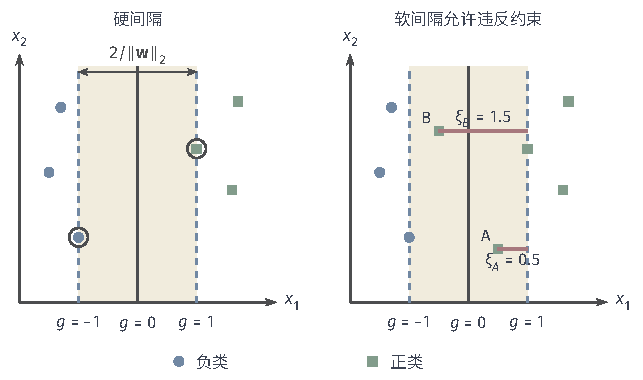
\includegraphics[width=108.850mm]{figures/04-classic-models/00-shared/tikz/classification-svm-margin/figure.pdf}
  \caption{硬间隔与软间隔的教学示意，坐标无量纲。蓝圆为负类，赭方为正类；两个面板都给定$\bm{w}=(1,0)^{\top}$、$b=-2$，黑色实线为决策边界$g=0$，蓝色虚线为间隔边界$g=\pm1$。单侧规范间隔为$1/\lVert\bm{w}\rVert_2=1$，两虚线总宽为$2/\lVert\bm{w}\rVert_2=2$；左图圈出间隔上的样本。右图红色线段直接标出松弛量：A位于$x_1=2.5$，正确分类但在间隔内，$\xi_A=0.5$；B位于$x_1=1.5$，已被错分，$\xi_B=1.5$。右图仅说明给定分界面下的最小松弛量，并非优化后的SVM最优解。}
  \label{fig:classification-svm-margin}
\end{figure}

消去$\bm{\xi}$，式\eqref{eq:classification-svm-soft-primal}等价于
\begin{equation}
  \min_{\bm{w},b}\quad
    \frac12\lVert\bm{w}\rVert_2^2
    +\lambda_{\mathrm{s}}\sum_{i=1}^n
       \max\{0,1-y_i g(\bm{x}_i)\}.
  \label{eq:classification-svm-hinge-objective}
\end{equation}
其中$\ell(z)=\max\{0,1-z\}$是\term{合页损失}（hinge loss）：达到目标间隔以后不再奖励更大的得分，间隔不足时线性增加惩罚。错误一侧的损失继续线性增加而不截断，保持了凸性。它把“最大间隔加违规代价”与“平方范数正则化加经验损失”联系起来。

惩罚参数的数值还依赖损失是求和还是取平均。将式\eqref{eq:classification-svm-hinge-objective}除以$n\lambda_{\mathrm{s}}$，等价目标是平均合页损失加$\lVert\bm{w}\rVert_2^2/(2n\lambda_{\mathrm{s}})$。所以在不同样本量或不同软件约定之间比较超参数时，应先统一归一化方式。较大的$\lambda_{\mathrm{s}}$允许模型付出更大范数来降低训练损失，较小的值更重视范数控制；范数和损失的这种取舍是否适合任务，需要结合数据、表示与验证结果判断。

软间隔的乘子上界来自松弛变量的最优性条件。分别为$1-\xi_i-y_i g(\bm{x}_i)\le0$与$-\xi_i\le0$引入$\alpha_i,\mu_i\ge0$，拉格朗日函数为
\[
  \begin{aligned}
    L={}&\frac12\lVert\bm{w}\rVert_2^2
       +\lambda_{\mathrm{s}}\sum_i\xi_i\\
      &+\sum_i\alpha_i
        \bigl[1-\xi_i-y_i(\bm{w}^{\top}\bm{x}_i+b)\bigr]
       -\sum_i\mu_i\xi_i.
  \end{aligned}
\]
关于$\bm{w},b$的驻点条件仍是式\eqref{eq:classification-svm-stationarity}，关于每个$\xi_i$则要求
\[
  \lambda_{\mathrm{s}}-\alpha_i-\mu_i=0.
\]
结合$\mu_i\ge0$，得到$0\le\alpha_i\le\lambda_{\mathrm{s}}$。取$\bm{w}=\bm{0}$、$b=0$和所有$\xi_i>1$可以严格满足两组不等式，因此不论数据是否可分，Slater条件都成立。消去原始变量后有
\begin{equation}
  \begin{aligned}
    \max_{\bm{\alpha}}\quad&
      \sum_{i=1}^n\alpha_i
       -\frac12\sum_{i,j=1}^n
         \alpha_i\alpha_j y_i y_j
         \bm{x}_i^{\top}\bm{x}_j\\
    \text{s.t.}\quad&
      \sum_{i=1}^n\alpha_i y_i=0,\\
    &0\le\alpha_i\le\lambda_{\mathrm{s}},
      \qquad i=1,\ldots,n.
  \end{aligned}
  \label{eq:classification-svm-soft-dual}
\end{equation}
对偶可行域非空且紧，目标连续，所以对偶最优值可以取得。原始形式同样有最优解；两类非空时，限制目标的水平集可控制$\bm{w}$与$\bm{\xi}$，再由两类约束控制$b$。

软间隔的互补松弛关系多了一组：
\begin{equation}
  \begin{aligned}
    &\alpha_i^{\ast}(m_i^{\ast}-1+\xi_i^{\ast})=0,\\
    &(\lambda_{\mathrm{s}}-\alpha_i^{\ast})\xi_i^{\ast}=0,\\
    &m_i^{\ast}\ge1-\xi_i^{\ast},\qquad \xi_i^{\ast}\ge0.
  \end{aligned}
  \label{eq:classification-svm-soft-kkt}
\end{equation}
联合原始与对偶可行性，可以逐项读出
\begin{equation}
  \begin{aligned}
    \alpha_i^{\ast}=0
      &\ \Longrightarrow\
        \xi_i^{\ast}=0,\quad m_i^{\ast}\ge1,\\
    0<\alpha_i^{\ast}<\lambda_{\mathrm{s}}
      &\ \Longrightarrow\
        \xi_i^{\ast}=0,\quad m_i^{\ast}=1,\\
    \alpha_i^{\ast}=\lambda_{\mathrm{s}}
      &\ \Longrightarrow\
        m_i^{\ast}=1-\xi_i^{\ast}\le1.
  \end{aligned}
  \label{eq:classification-svm-soft-cases}
\end{equation}
边界上的样本可以出现在三种乘子状态中：$\alpha_i^{\ast}=0$允许$m_i^{\ast}=1$，$\alpha_i^{\ast}=\lambda_{\mathrm{s}}$也允许$\xi_i^{\ast}=0$且$m_i^{\ast}=1$。反过来，$m_i^{\ast}>1$必有$\alpha_i^{\ast}=0$，$m_i^{\ast}<1$必有$\alpha_i^{\ast}=\lambda_{\mathrm{s}}$，而$m_i^{\ast}=1$时乘子可以是盒约束中的任意值，只要整体KKT系统成立。达到上界的乘子因此可能对应边界点、间隔内的正确样本或错分样本，需要结合$m_i^{\ast}$才能区分。

范数项依然只对$\bm{w}$严格凸，足以保证最优权重唯一，却不能保证偏置唯一。一个简单反例是两个输入都为零，标签分别为$+1$与$-1$。此时$\bm{w}^{\ast}=\bm{0}$，任意$b\in[-1,1]$都使总合页损失为$2$，因此都最优。该情形也说明，软间隔可能得到常值得分；只有$\bm{w}\ne\bm{0}$时，才可以继续用$1/\lVert\bm{w}\rVert_2$解释规范间隔的几何宽度。

若存在$0<\alpha_k^{\ast}<\lambda_{\mathrm{s}}$的\term{自由支持向量}（free support vector），它既参与决策又未碰到乘子上界，可用$m_k^{\ast}=1$恢复偏置。若没有这种样本，就应使用KKT给出的偏置区间。令$h_i=\sum_j\alpha_j^{\ast}y_j\bm{K}_{j,i}$，则$\alpha_i^{\ast}=0$要求$y_i(h_i+b)\ge1$，$\alpha_i^{\ast}=\lambda_{\mathrm{s}}$要求$y_i(h_i+b)\le1$。正标签的前一条件与负标签的后一条件给出下界，另两种组合给出上界；从两组界的交集中选择一个$b$，才是完整的恢复规则。该区间不一定收缩为单点。

SMO的一元目标与误差公式不变，但可行区间必须同时保证两个乘子都位于盒子内。令$s=y_i y_j$，新的$\alpha_j$区间为
\begin{equation}
  \begin{aligned}
    s=+1:\quad
    L&=\max\{0,\alpha_i^{(t)}+\alpha_j^{(t)}
                    -\lambda_{\mathrm{s}}\},\\
    H&=\min\{\lambda_{\mathrm{s}},
                    \alpha_i^{(t)}+\alpha_j^{(t)}\};\\
    s=-1:\quad
    L&=\max\{0,\alpha_j^{(t)}-\alpha_i^{(t)}\},\\
    H&=\min\{\lambda_{\mathrm{s}},
           \lambda_{\mathrm{s}}+\alpha_j^{(t)}-\alpha_i^{(t)}\}.
  \end{aligned}
  \label{eq:classification-svm-smo-soft-interval}
\end{equation}
这是由盒约束与等式约束共同截出的区间，通常小于$[0,\lambda_{\mathrm{s}}]$。使用式\eqref{eq:classification-svm-smo-update}剪裁并回代即可；当$\eta=0$时，这里的区间总是有限，可以直接比较端点目标。偏置仍按式\eqref{eq:classification-svm-smo-bias}计算，但优先使用更新后满足$0<\alpha_i<\lambda_{\mathrm{s}}$或$0<\alpha_j<\lambda_{\mathrm{s}}$的样本；二者都不自由时，可暂取两个候选偏置的平均，停止时再按全体KKT条件核验。

在可分数据上，足够大的有限惩罚就能使软间隔与硬间隔精确对应。取任意硬间隔最优乘子$\bm{\alpha}^{\mathrm{h}}$，若$\lambda_{\mathrm{s}}>\max_i\alpha_i^{\mathrm{h}}$，则硬间隔原始解连同$\bm{\xi}=\bm{0}$、$\bm{\alpha}^{\mathrm{h}}$和$\mu_i=\lambda_{\mathrm{s}}-\alpha_i^{\mathrm{h}}>0$满足软间隔KKT。由强对偶它也是软间隔最优解，而且正的$\mu_i$迫使所有最优松弛量为零。若数据不可分，则无论把惩罚增大到多少，都不能恢复一个本来就不存在的硬间隔可行解。

\paragraph{$\nu$-SVM：调节间隔与违反比例}
\label{sec:classification-svm-nu-extension}
软间隔惩罚系数衡量一单位间隔违反有多昂贵，却不能直接读成“允许多少训练样本违反间隔”。若希望调节参数与训练中的间隔错误比例、支持向量比例建立联系，可以考虑\term{$\nu$-SVM}（nu-support vector machine）。它把间隔阈值$\rho\geq0$也作为变量，在目标中用参数$\nu$奖励更大的阈值，同时惩罚平均松弛量：
\begin{equation}
  \begin{aligned}
    \min_{\bm{w},b,\rho,\bm{\xi}}\quad&
      \frac12\lVert\bm{w}\rVert_2^2-\nu\rho
      +\frac1n\sum_{i=1}^n\xi_i\\
    \text{满足}\quad&
      y_i(\bm{w}^{\top}\phi(\bm{x}_i)+b)\geq\rho-\xi_i,\\
    &\xi_i\geq0,\qquad \rho\geq0.
  \end{aligned}
  \label{eq:classification-nu-svm}
\end{equation}
消去原始变量后，可学习的仍是训练样本的非负系数，但对偶变为
\[
  \begin{aligned}
    \max_{\bm\alpha}\quad&-\frac12\sum_{i,j}\alpha_i\alpha_jy_iy_jK(\bm x_i,\bm x_j),\\
    \text{满足}\quad&0\leq\alpha_i\leq1/n,\quad
       \sum_i\alpha_i y_i=0,\quad\sum_i\alpha_i\geq\nu.
  \end{aligned}
\]
最后一个不等式来自原始问题中的$\rho\geq0$。固定核后可用凸二次规划求系数，再由原始约束和互补松弛恢复偏置及间隔阈值，预测仍对核展开得分取符号。这个目标与软间隔相似，却不是只把惩罚参数换一个名字。

使用时还需结合类别数量检查参数范围：两类训练样本数为$n_+$、$n_-$时，应限制$0<\nu\leq2\min(n_+,n_-)/n$。以下讨论达到精确最优、且最优间隔阈值$\rho^\ast>0$的非退化情形。记最优得分为$g^\ast$，满足$y_i g^\ast(\bm{x}_i)<\rho^\ast$的训练样本称为间隔违反样本；其中也包括已经分类正确、但尚未达到目标间隔的样本。此时，$\nu$是间隔违反样本比例的上界，也是非零对偶系数所对应支持向量比例的下界\scite{scholkopf2000nu}。

这两个方向可以从KKT条件读出。为间隔约束引入乘子$\alpha_i\geq0$。关于松弛变量的驻点条件给出$\alpha_i\leq1/n$；关于$\rho$的驻点条件与$\rho^\ast>0$的互补松弛关系给出
\[
  0\leq\alpha_i^\ast\leq\frac1n,
  \qquad \sum_{i=1}^{n}\alpha_i^\ast=\nu.
\]
这里仍有偏置的驻点条件$\sum_i\alpha_i^\ast y_i=0$，所以正、负两类的乘子总量相同，均为$\nu/2$。每项乘子至多为$1/n$，正类总量因而不超过$n_+/n$，负类总量不超过$n_-/n$。将这两项上界与$\nu/2$比较，就得到前面要求的$\nu\leq2\min(n_+,n_-)/n$；少数类的样本数量限制了两类能够共同承担的乘子总量。这也说明，上述类别数量条件与后面的比例解释都应结合当前模型及最优阈值条件检查。

令$E_\nu=\{i:y_i g^\ast(\bm{x}_i)<\rho^\ast\}$、$S_\nu=\{i:\alpha_i^\ast>0\}$。间隔违反样本的最优松弛量为正，因而乘子必须达到上界$1/n$；另一方面，要把每项至多$1/n$的非负乘子累加到$\nu$，至少需要$n\nu$个非零项。于是
\begin{equation}
  \frac{|E_\nu|}{n}\leq\nu\leq\frac{|S_\nu|}{n}.
  \label{eq:classification-nu-svm-proportions}
\end{equation}
例如，$n=100$、$\nu=0.2$且上述条件满足时，间隔违反样本至多有20个，支持向量至少有20个；这既不表示恰有20个错分样本，也不是对测试错误率的保证。若最优$\rho=0$，这里依据$\sum_i\alpha_i^\ast=\nu$得到的比例解释不能直接沿用。

固定核后，$\nu$-SVM与软间隔SVM使用同一得分族。它改变间隔的选取方式，不增加非线性特征，也仍需要检查核尺度、类别不平衡和独立验证误差。

\subsubsection{多分类：组合二分类器或联合学习}

\label{sec:classification-svm-multiclass}

二分类模型只需判断得分的正负；当候选类别超过两个时，还需要规定多个类别怎样竞争。一个直观的办法是把多分类问题拆成若干个“二选一”的小问题再把答案汇总；另一个办法是让所有类别在同一个优化目标里直接竞争。硬间隔、软间隔和核方法都能作为构件，但“拆成多个二分类器”与“直接优化多类间隔”会得到不同的训练目标。

现在将标签改为$y_i\in\{1,\ldots,C\}$，其中$C\ge3$，类别索引记为$c$。最直接的推广仍然保留二分类求解器，只改变训练任务的组织方式。\term{一对一}（one-vs-one，OvO）为每对类别$c<c'$训练一个分类器$h_{c,c'}$，仅使用标签为$c$或$c'$的样本，共有$C(C-1)/2$个模型。每个模型在这两个类别之间投一票，预测为
\[
  \hat y(\bm{x})
  =\argmax_{c\in\{1,\ldots,C\}}
     \sum_{c_1<c_2}\mathbb{1}\{h_{c_1,c_2}(\bm{x})=c\}.
\]
其中$c_1,c_2\in\{1,\ldots,C\}$，票数并列时采用预先约定的固定规则，例如选择较小类别编号。不同类别对可能作出不相容的局部判断，投票负责把这些判断汇总成一个输出，并不要求它们对应同一个全局概率模型。

\term{一对其余}（one-vs-rest，OvR）为每个类别$c$构造二分类标签：原标签为$c$时取$+1$，其余取$-1$。训练$C$个实值得分函数$g_c$后，使用
\[
  \hat y(\bm{x})=\argmax_{c\in\{1,\ldots,C\}}g_c(\bm{x}),
\]
并固定平局规则。即使所有得分都为负，或多个类别得分为正，这个最大值规则仍能给出类别。它比较的是独立模型的得分，得分尺度与训练中的类别不平衡可能影响比较，因此通常需要统一预处理、损失约定并评估各类别的错误，若要比较类别后验，还需建立并检验相应的概率映射。

图\ref{fig:classification-svm-multiclass}把四个类别展开成具体训练任务。沿着一列看，一对一中的每个类别只参与三个任务；一对其余中，每个样本都参与四个任务，但只有一个任务把它标为正类。沿着一行看，前者忽略不属于当前类别对的样本，后者把所有其他类别合并为负类。这种训练标签的差异，决定了两个组合器面对的子问题并不相同。

\begin{figure}[htbp]
  \centering
  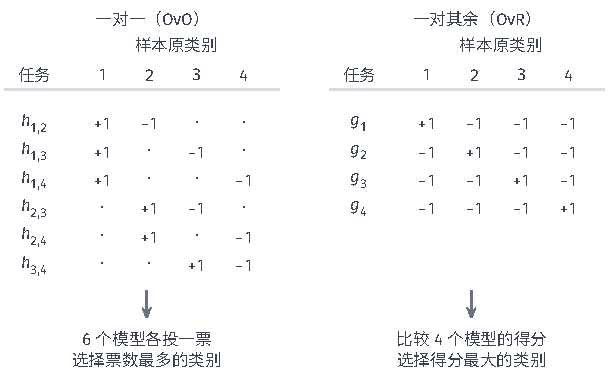
\includegraphics[width=104.027mm]{figures/04-classic-models/00-shared/tikz/classification-svm-multiclass/figure.pdf}
  \caption{四分类任务中的两种二分类组合方式。各行对应一个待训练模型，各列对应样本的原类别；$+1$和$-1$是为该任务重新编码的标签，点号表示该类样本不参与训练。一对一训练6个模型并汇总类别选票，一对其余训练4个模型并比较实值得分。图中给出训练与预测规则，不预设两种方法会产生相同的分类结果。}
  \label{fig:classification-svm-multiclass}
\end{figure}

OvO的模型多、单个训练子问题小，OvR的模型少、每个子问题使用全部样本；总成本因而取决于数据分布和求解器，不能只比较模型个数。

如果希望组合器能够容忍若干二分类判断错误，可以为每个类别安排一个彼此分离的编码。\term{纠错输出码}（error-correcting output codes，ECOC）将类别$c$表示成长度为$q$的码字$\bm{M}_{c,:}$，其中码本$\bm{M}\in\{-1,+1\}^{C\times q}$的各行互不相同，每列同时含两种符号。第$j$列定义一个二分类任务，样本$i$的训练标签为$\bm{M}_{y_i,j}$；训练后得到$q$个二分类器$h_j$。预测时形成输出码$\bm{h}(\bm{x})=(h_1(\bm{x}),\ldots,h_q(\bm{x}))$，再选择最近的类别码字：
\begin{equation}
  \begin{aligned}
    \hat y(\bm{x})
      &=\argmin_c d_{\mathrm{H}}
          \bigl(\bm{h}(\bm{x}),\bm{M}_{c,:}\bigr),\\
    d_{\mathrm{H}}(\bm{u},\bm{v})
      &=\sum_{j=1}^q\mathbb{1}\{u_j\ne v_j\}.
  \end{aligned}
  \label{eq:classification-svm-ecoc}
\end{equation}
这里的\term{汉明距离}（Hamming distance）就是两个码字不一致的位置数。要表示$C$个不同类别，至少需要$q\ge\lceil\log_2 C\rceil$；加入冗余位的目的，是增大不同类别之间的距离，而不只是增加分类器个数。Dietterich与Bakiri系统研究了这种将多分类转换为多个编码位学习问题的方法\scite{dietterich1995ecoc}。

纠错能力可以直接证明。记码本最小类间距离为$\Delta_{\min}$，若真实类别为$c$，输出码与$\bm{M}_{c,:}$相差$e$位，则对任意$c'\ne c$，三角不等式给出
\[
  d_{\mathrm{H}}(\bm{h},\bm{M}_{c',:})
  \ge d_{\mathrm{H}}(\bm{M}_{c,:},\bm{M}_{c',:})-e
  \ge\Delta_{\min}-e.
\]
只要$2e<\Delta_{\min}$，真实码字就比任何其他码字更近。因此至多$\lfloor(\Delta_{\min}-1)/2\rfloor$位错误可以被最近码字解码纠正。这个结论以实际错误位数为条件；若多个二分类器因为相同特征缺陷而同时犯错，冗余编码本身并不能保证错误位数足够小。

另一条路线不再训练彼此独立的二分类器，而是直接优化类别之间的竞争关系。\term{Crammer--Singer多类SVM}（Crammer--Singer multiclass SVM）要求真实类别得分至少比每个错误类别高一个单位间隔，从而在同一目标中学习所有类别权重。

令$\bm{W}=[\bm{w}_1,\ldots,\bm{w}_C]\in\mathbb{R}^{d\times C}$，使用带偏置的版本$g_c(\bm{x})=\bm{w}_c^{\top}\bm{x}+b_c$，相应优化问题为\scite{crammer2001multiclass}。
\begin{equation}
  \begin{aligned}
    \min_{\bm{W},\bm{b},\bm{\xi}}\quad&
      \frac12\sum_{c=1}^C\lVert\bm{w}_c\rVert_2^2
       +\lambda_{\mathrm{s}}\sum_{i=1}^n\xi_i\\
    \text{s.t.}\quad&
      g_{y_i}(\bm{x}_i)-g_c(\bm{x}_i)\ge1-\xi_i,
      \quad c\ne y_i,\\
    &\xi_i\ge0,\qquad i=1,\ldots,n.
  \end{aligned}
  \label{eq:classification-svm-crammer-singer}
\end{equation}
不使用偏置时固定$\bm{b}=\bm{0}$；使用偏置时，可加$\sum_c b_c=0$去掉共同平移的不识别性。消去松弛变量后，每个样本的损失为$\max\{0,\max_{c\ne y_i}[1+g_c(\bm{x}_i)-g_{y_i}(\bm{x}_i)]\}$，即惩罚最强错误竞争者超过允许差距的程度。预测仍取$\argmax_c g_c(\bm{x})$，并可将权重推广到核特征空间。这一凸目标可以用分解法求对偶，线性形式也可用次梯度训练：对每个样本先找得分最高的错误类别；若它违反单位间隔，损失对正确类权重贡献$-\lambda_{\mathrm s}\bm x_i$，对该竞争类贡献$+\lambda_{\mathrm s}\bm x_i$，其余类为零。累计全部样本的贡献，再加上范数项的梯度$\bm w_c$，沿负方向更新各类权重；偏置只累计损失项的相应标量贡献。最强竞争者并列时任选一个仍给出次梯度。这样，训练直接提高正确类相对于错误竞争者的得分，而不独立拟合每个“该类对其余类”的任务。

这一联合目标明确比较了类别之间的相对间隔，OvR则分别比较“该类”与“其余类”。二者的约束数、求解器和数据分解方式不同，训练成本与预测质量也要在相同数据和调参预算下评估。联合建模提供了不同的归纳偏好，并不构成相对于OvO或OvR的普遍性能排序。

这些多分类构造也改变了候选边界。线性OvR与联合多类SVM都按仿射得分的最大值判类，因此每类区域仍是半空间的交。OvO和ECOC先进行若干二分类再解码，各类区域可以由多个分区拼合。这种拼合能够表达单个半空间之外的区域，其能力由可用的二分类划分与解码方式共同决定。训练中的间隔保证若要用于整体分类，还需把错误的二分类比较与最终解码联系起来，不能直接取某个成员的风险作为组合器的风险。



\subsection{模型对比与总结}
\label{sec:classification-geometry-summary}

在同一组输入特征上的二分类问题中，LDA、感知机与线性SVM都用仿射得分形成半空间判断。只看边界的线性形状，无法知道权重来自哪里：LDA从类均值、共享协方差和先验形成得分；感知机在错分点出现时调整当前权重；SVM用范数与间隔损失比较候选边界。相同的得分形式因而不意味着相同的学习目标，也不意味着会从同一训练集选出相同边界。

若类条件高斯与共享协方差近似可信，LDA可以同时利用类内相关性并形成后验概率；样本不足以估计完整协方差时，需要收缩或更受限的协方差表示。感知机省去分布拟合，适合直接使用错误反馈作增量更新，但停止预算、访问顺序和历史参数的返回方式会影响结果。SVM在给定表示中显式权衡间隔与违反程度，代价是求解相应优化问题并选择惩罚强度。表\ref{tab:classification-linear-comparison}汇总这些选择条件。

\begin{table}[htbp]
  \centering
  \small
  \begin{tabularx}{\linewidth}{@{}>{\RaggedRight\arraybackslash}p{18mm}>{\RaggedRight\arraybackslash}X>{\RaggedRight\arraybackslash}X@{}}
    \toprule
    模型 & 边界由什么决定 & 主要条件与代价 \\
    \midrule
    LDA & 类均值、共享协方差与类先验 & 高斯假设支持概率解释；协方差估计需足够样本或正则化。 \\
    感知机 & 错分样本触发的权重更新 & 依赖访问顺序；不可分时需停止规则或变体。 \\
    线性 SVM & 范数与间隔损失的权衡 & 硬间隔要求可分；软间隔需选择惩罚强度。 \\
    核 SVM & 特征空间中的间隔 & 核定义相似性；训练与预测开销受样本数和支持向量数影响。 \\
    \bottomrule
  \end{tabularx}
  \caption{线性与核化分类器的比较。LDA 一行指共享协方差的高斯生成模型；Fisher 投影本身不要求高斯分布。比较时还需固定输入表示与评价口径。}
  \label{tab:classification-linear-comparison}
\end{table}

原坐标中的类别关系不能由仿射得分表达时，重复更新参数或调整惩罚都不能补上这种限制。核Fisher判别、核感知机与核SVM改用特征空间内积，分别保留类统计量比较、错分反馈与间隔选择这三种依据。核与输入尺度决定提供哪些关系，各自的学习目标再决定怎样使用这些关系。预测时是否需要保存全部训练样本、更新样本或支持向量，也随方法而异。

若还需要稀疏的概率核预测，相关向量机改用逐基函数的高斯先验与精度学习，其结构与训练见第\ref{sec:classification-rvm}节；它与SVM共享核展开形式，但不使用同一个间隔目标。

\section{基于邻域的分类}
\label{sec:classification-instances}

前面的线性分类器用一组全局权重决定边界。如果同一类别分布在几个相隔的区域，一条直线可能无法把它们同时与另一类分开。我们也可以暂不规定整条边界的形状，而在新输入附近寻找带标签的样本，用这些局部记录判断类别。这是$k$-NN分类的做法：保存训练实例，按距离找出邻居，再聚合标签。与回归中的响应平均相比，分类采用多数投票或局部类别比例。近邻表示和检索的基础见第\ref{sec:classic-overview-neighborhood}节，回归对应形式见第\ref{sec:regression-knn}节。

\subsection{$k$近邻分类（$k$-NN）}
\label{sec:classification-knn}

局部比较避开了预先选择全局边界，却留下一个问题：附近只取一个样本，还是让多个样本一起判断？最近的样本也可能带有噪声标签；增加邻居能平均这种波动，但范围过大又会把别处的类别混进来。近邻数因此决定了我们用多大范围的标签来描述当前输入。

Cover与Hart在1967年的论文中回顾了Fix与Hodges始于1951年报告的近邻判别研究：在所研究的条件下，让近邻数随样本量增长、同时让其占比趋于零，可以获得一致性。Cover与Hart则分析了始终只取一个最近邻时，极限错误率与贝叶斯风险之间的界。前者研究增长近邻数怎样平均标签噪声，后者刻画单个邻居仍保留多少判别信息\scite{coverhart1967}。

\subsubsection{模型结构}
\label{sec:classification-knn-structure}

给定训练集$D_n=\{(\bm{x}_i,y_i)\}_{i=1}^n$、距离$\rho$以及$1\leq k\leq n$，用$N_k(\bm{x})\subseteq\{1,\ldots,n\}$表示查询$\bm{x}$的$k$个最近邻索引。预测规则为
\begin{equation}
  \hat h_{n,k}(\bm{x})
  =\argmax_{c\in\{1,\ldots,C\}}
  \sum_{i\in N_k(\bm{x})}\mathbb{1}\{y_i=c\}.
  \label{eq:classification-knn-vote}
\end{equation}
距离相同时，按预先约定、独立于标签的顺序选取邻居；类别票数并列时也使用固定规则。多分类在奇数$k$时也可能出现票数并列，因此两种平局都需要明确规则。

式\eqref{eq:classification-knn-vote}也可以理解为估计查询附近的类别比例：
\begin{equation}
  \hat\eta_{n,c}(\bm{x})
  =\frac{1}{k}\sum_{i\in N_k(\bm{x})}\mathbb{1}\{y_i=c\},
  \qquad
  \hat h_{n,k}(\bm{x})=\argmax_c\hat\eta_{n,c}(\bm{x}).
  \label{eq:classification-knn-posterior}
\end{equation}
比例估计解释了投票为什么可能有效：若邻域内的条件类别分布变化不大，邻居标签就能提供关于当前输入的统计证据。局部比例的误差取决于邻域大小与标签噪声，概率质量需通过样本外数据检验。

图~\ref{fig:classification-knn-neighborhood}固定训练点和查询，只改变参与投票的近邻数。取查询$\bm{x}=(0,0)$，样本1、3、4、6属于类1，其余样本属于类2。按欧氏距离计算，七个样本到查询的平方距离依编号为$1,2,2.5,4.25,5,9,10.25$，因此编号也表示由近到远的次序。

$k=1$时只有样本1投票，查询被判为类1；$k=5$时样本1至5投票，其中类1有三票、类2有两票，预测仍为类1。两幅图中的圆分别经过第1和第5个邻居，半径为$1$和$\sqrt5$。圆表示当前查询的证据范围，整个平面上的分类边界则由各查询的投票共同决定。比较两个$k$的准确性还需要查询的真实标签。

\begin{figure}[htbp]
  \centering
  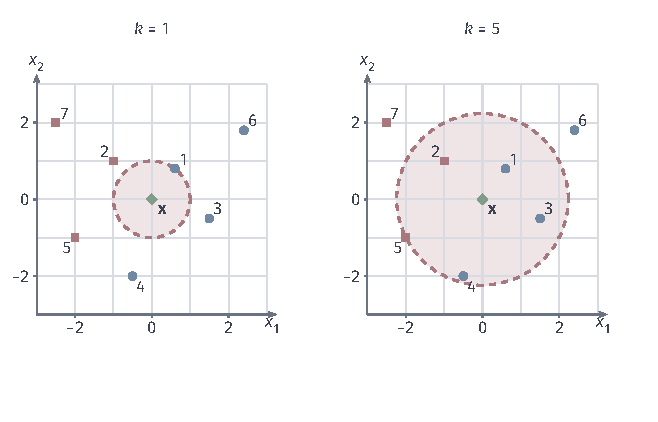
\includegraphics[width=111.404mm]{figures/04-classic-models/00-shared/tikz/classification-knn-neighborhood/figure.pdf}
  \caption{同一查询下的近邻范围与投票变化。教学构造取$n=7$、$d=2$、无量纲坐标和欧氏距离，查询为$\bm{x}=(0,0)$；两图的样本、编号及坐标尺度完全相同。蓝色圆点表示类1，红色方点表示类2，绿色菱形表示查询，红色虚线圆表示包含边界的近邻范围。左图$k=1$、半径$1$，蓝、红票数为$1:0$；右图$k=5$、半径$\sqrt5$，票数为$3:2$，因此判为蓝色类。各邻居等权投票，距离和票数均无并列；点的位置、标签与参数均为人为设定，不代表真实数据实验。}
  \label{fig:classification-knn-neighborhood}
\end{figure}

\subsubsection{参数学习}
\label{sec:classification-knn-learning}

基本$k$-NN分类没有固定维数参数的优化过程，但需要确定输入表示、距离、近邻数及检索方式。“非参数化”是指预测关系不局限于一个固定有限维参数族；它仍有超参数，预处理和模型选择也属于学习。

距离决定哪些样本会参与投票。对数值特征，欧氏距离$\rho(\bm{x},\bm{z})=\lVert\bm{x}-\bm{z}\rVert_2$容易计算，却会放大数值范围较大的坐标。收入和年龄共同作为特征时，直接使用原始单位会让收入差异主导距离。标准化、按业务意义设定尺度或学习特征权重都可改变这一点；不同特征的重要性可通过任务知识或训练数据确定。标准化参数只能从训练集估计，交叉验证时应在各训练折内重新拟合，避免验证信息提前进入距离。

类别型特征可采用\term{汉明距离}（Hamming distance），按不同取值的坐标数比较，而不能把任意类别编码的数字差当成有意义的远近。文本的TF--IDF等稀疏向量常比较余弦相似度，强调方向而非长度；$1$减余弦相似度一般不满足三角不等式，不能直接套用所有度量空间结论。对非零向量作单位长度归一化后，按余弦相似度排序与按欧氏距离排序等价，此时可用欧氏空间中的解释。

若特征之间相关，可以考虑\term{马氏距离}（Mahalanobis distance），用协方差调整方向上的尺度：
\begin{equation}
  \rho_{\mathrm{M}}(\bm{x},\bm{z})^2
  =(\bm{x}-\bm{z})^\top
   \bm{\Sigma}^{-1}(\bm{x}-\bm{z}),
  \label{eq:classification-mahalanobis}
\end{equation}
其中$\bm{\Sigma}\in\mathbb{R}^{d\times d}$须正定。样本不足时协方差估计可能奇异，需要正则化；整体协方差也不一定符合分类所需的相似性。

近邻数$k$控制局部平均的范围。$k=1$时，一个错误标签就会影响邻近查询；增加邻居可平均这类波动，也会混入更远区域并削弱局部细节。因此$k$的选择需要结合类别比例、局部密度与距离表示，在训练集内部验证。$k\approx\sqrt n$可以作为搜索起点，最终选择依据相同评价条件下的误差。

检索代价需要区分距离计算与邻居选择。对一个$d$维稠密查询，朴素扫描$n$个训练样本计算距离需$O(nd)$；若再把所有距离排序，总代价为$O(nd+n\log n)$。采用线性选择算法得到最小的$k$项，再作投票，可达$O(nd+n+k)$；使用大小为$k$的堆则需$O(nd+n\log(k+1)+k)$。因此，通常所说的$O(nd)$朴素预测复杂度隐含了无需完整排序的选择方法。训练集的存储为$O(nd)$，批量计算、硬件、精度要求和延迟预算共同决定这种实现的可用规模。

KD树或球树（ball tree）等精确索引通过空间划分排除不可能更近的样本。低维且分布有利时，它们可以减少访问量；最坏情形仍会检查大部分样本。索引保留原预测规则，选择时比较建索引成本、内存和实际查询时间，维数的影响需结合数据分布测量。

对高维大规模数据，还可以用\term{近似最近邻检索}（approximate nearest-neighbor search）交换少量检索误差与计算收益。局部敏感哈希（locality-sensitive hashing, LSH）让相近向量较可能进入同一哈希桶；分层可导航小世界图（hierarchical navigable small world, HNSW）沿多层邻接图逐步寻找候选；倒排文件与乘积量化（inverted file with product quantization, IVF--PQ）先缩小候选分区，再用压缩编码近似距离。这些方法的搜索预算和压缩程度会改变邻居集合，需同时检查邻居召回率与最终分类误差。以下理论以精确检索为前提，不直接覆盖任意近似索引。

\subsubsection{理论分析}
\label{sec:classification-knn-theory}

\paragraph{表达能力}
固定$n$、$k$及欧氏距离后，一个候选规则由$n$个锚点的位置与类别共同规定：查询时取最近的$k$个锚点，再按既定平局规则比较票数。考察所有可能的锚点位置与类别，才能说明这一规则族能够表达哪些目标。每个候选都是分段常值函数；邻居集合只在锚点的等距平面处改变，同一邻居集合给出相同票数。

锚点可以让一个类别占据几个分离的区域。例如，$k=1$时将四个锚点放在前面的异或输入$(\pm1,\pm1)$上，并赋予相应类别，坐标轴便把平面划成四个最近锚点区域；四个开象限的类别可全部吻合异或目标。更一般地，若各目标类别对应的输入集合都紧致，不同类别集合之间的距离至少为$\Delta>0$，可在每类选取有限个锚点，使该类每个输入到同类锚点的距离小于$\Delta/2$。当$n$足以容纳这一覆盖时，异类锚点至少相距$\Delta$，这组1-NN候选便能精确表示整个目标支持上的类别。

有限锚点仍限制了边界形状。在平面上按单位圆的内外区分类别时，有限条等距直线不能拼成整条圆周，任一有限锚点候选都无法处处吻合这个目标。若输入表示又把不同目标类别映到同一点，所有基于该表示的候选都会对它们给出相同判断。

票数比例还有独立于分区形状的限制。固定$k$时，每类比例只能取$0,1/k,\ldots,1$，不能精确表示任意后验概率。例如两类、$k=3$且真实正类后验恒为$3/10$时，任一候选在每个输入处的概率差都至少为$1/30$。增加锚点数可以提供更多空间分区，却不改变这一固定的概率刻度。

\paragraph{收敛性}
标准$k$-NN保存训练实例，给定距离和邻居数后没有参数优化过程，也就没有迭代找到最优参数的保证或速率。精确检索与投票能直接执行已定义的预测规则；朴素稠密实现为每个查询计算$n$个距离，约需$O(nd)$运算，再选择近邻。近似检索降低计算成本时，漏检或错检造成的误差必须另行评价。

\paragraph{泛化性}
位置接近仍可能伴随标签差异。两个相同输入在类别重叠或标签噪声下，也可独立产生不同标签。因此先规定训练集、查询与标签的随机性，再将邻居位置的极限联系到条件类别分布和分类风险。

设训练样本与测试点$(\bm{X},Y)$独立同分布于$\mathbb{R}^d\times\{1,\ldots,C\}$，$P_X$为输入边缘分布，$C\geq2$。令
\begin{equation}
  \eta_c(\bm{x})=\mathbb{P}(Y=c\mid\bm{X}=\bm{x}),
  \qquad
  r^\ast(\bm{x})=1-\max_c\eta_c(\bm{x}).
  \label{eq:classification-local-bayes-risk}
\end{equation}
沿用\term{贝叶斯风险}（Bayes risk）记号$R^\ast=\mathbb{E}_{\bm{X}}r^\ast(\bm{X})$。为区分近邻规则在一份训练集上的风险和它对训练抽样的平均表现，分别记为
\begin{align}
  L_{n,k}(D_n)
  &=\mathbb{P}\{\hat h_{n,k}(\bm{X})\neq Y\mid D_n\},
  \label{eq:classification-knn-conditional-risk}\\
  R_{n,k}&=\mathbb{E}_{D_n}L_{n,k}(D_n).
  \label{eq:classification-knn-expected-risk}
\end{align}
若打破距离并列采用独立随机化，以上期望同时包含该随机化。下面的Cover--Hart界针对$R_{n,1}$的极限，不是任意有限$n$的风险上界，也不是每份训练集条件风险的逐一保证。

先看局部比例的估计偏差。给定邻居输入后，等权票数比例的条件期望为$k^{-1}\sum_{r=1}^k\eta_c(\bm x_{(r)})$。若存在常数$L_\eta\geq0$，使$|\eta_c(\bm x)-\eta_c(\bm z)|\leq L_\eta\|\bm x-\bm z\|_2$，并记最远邻居距离为$r_k(\bm x)$，则
\[
  \left|\frac1k\sum_{r=1}^k\eta_c(\bm x_{(r)})
                 -\eta_c(\bm x)\right|
       \leq L_\eta r_k(\bm x).
\]
这一式子只控制条件均值的偏差，标签抽样还会使实际票数波动；下面的风险结论需要把两者一起处理。

先说明足以支撑极限计算的一组分布条件。使用固定的欧氏距离，精确寻找最近邻，邻居选择不依赖标签；对$P_X$几乎处处的非原子点$\bm{x}$，各$\eta_c$在该点相对于$P_X$的支撑集连续。所谓原子点是$P_X(\{\bm{x}\})>0$的点，它不需要这里的连续性要求。该条件不要求输入分布有密度，更不要求每个欧氏空间位置都有正密度，但它也不只是“条件概率存在”。

\begin{lemma}[最近邻风险的极限]
  \label{lem:classification-nearest-neighbor-limit}
  在上述抽样、检索与连续性条件下，最近邻位置几乎必然趋于查询位置，并且
  \begin{equation}
    R_{1,\infty}:=\lim_{n\to\infty}R_{n,1}
    =\mathbb{E}_{\bm{X}}\left[
      1-\sum_{c=1}^{C}\eta_c(\bm{X})^2
    \right].
    \label{eq:classification-nearest-neighbor-limit}
  \end{equation}
\end{lemma}

\begin{proof}
  将训练集看作同一无穷独立样本序列的前$n$项。固定支撑集中的查询$\bm{x}$，用$I_n$表示最近邻索引，用$B(\bm{x},\varepsilon)$表示半径$\varepsilon>0$的开球。支撑集的定义保证该球有正概率，因此
  \[
    \mathbb{P}\{\|\bm{X}_{I_n}-\bm{x}\|_2\geq\varepsilon\}
    =\bigl[1-P_X(B(\bm{x},\varepsilon))\bigr]^n
    \longrightarrow0.
  \]
  最近邻距离随$n$不增，对$\varepsilon=1,1/2,1/3,\ldots$分别取极限，即得$\bm{X}_{I_n}\to\bm{x}$几乎必然成立。欧氏空间具有可数拓扑基，不在支撑集中的点可被可数个零概率开集覆盖，故支撑集本身具有$P_X$概率1。若$\bm{x}$为原子点，训练序列几乎必然在有限步后出现$\bm{x}$，此后最近邻距离一直为零。

  对非原子点，由连续性得到$\eta_c(\bm{X}_{I_n})\to\eta_c(\bm{x})$；对原子点，这个等式最终直接成立。最近邻索引只依赖输入及与标签独立的平局约定。给定查询和所有训练输入后，测试标签与选中的训练标签独立，选中标签属于$c$的概率为$\eta_c(\bm{X}_{I_n})$。故对训练集平均的条件错误率为
  \[
    r_n(\bm{x})
    =1-\sum_{c=1}^{C}\eta_c(\bm{x})
       \mathbb{E}\bigl[\eta_c(\bm{X}_{I_n})\bigr],
  \]
  这里的期望针对固定查询时的训练输入及邻居选择随机性。由于后验概率有界，可用支配收敛定理得到
  \[
    r_n(\bm{x})\longrightarrow
    r_\infty(\bm{x})
    :=1-\sum_{c=1}^{C}\eta_c(\bm{x})^2.
  \]
  再利用$0\leq r_n(\bm{x})\leq1$，对$\bm{x}$积分并交换极限与期望，就得到式\eqref{eq:classification-nearest-neighbor-limit}。
\end{proof}

极限中的平方项来自两次独立的类别抽取，而不是说最近邻标签本身几乎必然收敛。位置接近保证的是选中标签的条件分布接近查询的条件分布，单次标签抽样的波动仍然存在。

要平均掉这部分噪声，需要让参与投票的邻居数增加；要避免把远处结构混入，又需要邻居只占全部训练样本的越来越小一部分。令$k=k_n$满足$k_n\to\infty$且$k_n/n\to0$。Stone的非参数一致性结果在固定有限维欧氏空间中建立了近邻条件概率估计的积分收敛，也就是对训练集与查询取平均后，估计的绝对误差趋于零；这为后面的风险分析提供了依据\scite{stone1977consistent}。

对精确欧氏近邻，距离并列时可按与数据独立的随机排列选取，类别票数并列时按固定类别顺序决定。对每个$c$，这样的近邻估计满足
\begin{equation}
  \mathbb{E}_{D_n,\bm{X}}
  \bigl|\hat\eta_{n,c}(\bm{X})-\eta_c(\bm{X})\bigr|
  \longrightarrow0.
  \label{eq:classification-knn-posterior-consistency}
\end{equation}
这一结论对$\mathbb{R}^d$上任意固定联合分布成立，不需要前面为简化Cover--Hart证明而采用的逐点连续性条件。其一般证明使用欧氏空间的覆盖性质，不能只用一句普通大数定律代替，因为邻居样本是根据查询和输入位置选择出来的。

在前述连续性条件下，可以直接看出式\eqref{eq:classification-knn-posterior-consistency}的两个来源。给定训练输入，记
\[
  \bar\eta_{n,c}(\bm{x})
  =\frac{1}{k_n}\sum_{i\in N_{k_n}(\bm{x})}\eta_c(\bm{X}_i).
\]
邻居标签在给定输入后独立，所以
\[
  \mathbb{E}\!\left[
    |\hat\eta_{n,c}(\bm{x})-\bar\eta_{n,c}(\bm{x})|
    \,\middle|\,\bm{X}_1,\ldots,\bm{X}_n
  \right]\leq\frac{1}{2\sqrt{k_n}}.
\]
上界来自Bernoulli变量的方差不超过$1/4$及Cauchy--Schwarz不等式。它控制标签抽样波动。对任意有正概率的查询邻域，落入其中的样本比例几乎必然趋向该邻域的概率；由于$k_n/n\to0$，最终会有至少$k_n$个训练样本落入其中。因此，第$k_n$个邻居的距离趋于零。后验连续时，$\bar\eta_{n,c}(\bm{x})-\eta_c(\bm{x})$趋于零；在原子点，最终选中的$k_n$个输入都可等于该点。结合有界性与支配收敛，就得到这组较强正则性条件下的积分收敛。Stone的结论把同一估计分析扩展到了不连续后验。

已有的极限计算还需要与最优分类错误比较，才能说明近邻规则的预测保证。固定$k=1$时，Cover--Hart定理比较引理~\ref{lem:classification-nearest-neighbor-limit}中的极限局部错误与最优局部错误；让$k_n$增长时，则可用式\eqref{eq:classification-knn-posterior-consistency}控制相对于贝叶斯决策多出的错误。这两种风险保证都对训练集和独立测试点取平均。

\begin{theorem}[1-NN在二分类条件下的渐近期望风险界]
  \label{thm:classification-cover-hart-binary}
  在引理~\ref{lem:classification-nearest-neighbor-limit}的条件下，若$C=2$，则
  \begin{equation}
    R^\ast\leq R_{1,\infty}
    \leq2R^\ast(1-R^\ast)\leq2R^\ast.
    \label{eq:classification-cover-hart-binary}
  \end{equation}
\end{theorem}

\begin{proof}
  固定$\bm{x}$，记$p=\eta_1(\bm{x})$，则$\eta_2(\bm{x})=1-p$，$r^\ast(\bm{x})=\min(p,1-p)$。引理给出
  \begin{align*}
    r_\infty(\bm{x})
    &=1-p^2-(1-p)^2\\
    &=2p(1-p)\\
    &=2r^\ast(\bm{x})\bigl[1-r^\ast(\bm{x})\bigr].
  \end{align*}
  由于$0\leq r^\ast(\bm{x})\leq1/2$，有$2(1-r^\ast(\bm{x}))\geq1$，所以$r_\infty(\bm{x})\geq r^\ast(\bm{x})$。对输入取期望得到下界。对于上界，
  \begin{align*}
    R_{1,\infty}
    &=2R^\ast-2\mathbb{E}_{\bm{X}}[r^\ast(\bm{X})^2]\\
    &\leq2R^\ast-2(R^\ast)^2\\
    &=2R^\ast(1-R^\ast).
  \end{align*}
  不等式利用$\mathbb{E}[Z^2]\geq(\mathbb{E}Z)^2$，也就是对凹函数$2z(1-z)$使用Jensen不等式。再用$1-R^\ast\leq1$得到两倍上界。
\end{proof}

多分类时，不能沿用二类的精确表达式$2p(1-p)$，因为非最大类别的概率还可以在多个类别之间分配。需要控制的是：固定最大后验概率以后，其余类别的概率平方和最小能是多少。

\begin{theorem}[1-NN在多分类条件下的渐近期望风险界]
  \label{thm:classification-cover-hart-multiclass}
  在引理~\ref{lem:classification-nearest-neighbor-limit}的条件下，对任意有限$C\geq2$，
  \begin{equation}
    R^\ast\leq R_{1,\infty}
    \leq R^\ast\left(2-\frac{C}{C-1}R^\ast\right)
    \leq2R^\ast.
    \label{eq:classification-cover-hart-multiclass}
  \end{equation}
\end{theorem}

\begin{proof}
  固定$\bm{x}$并简记$r=r^\ast(\bm{x})$。取$c^\ast$使$\eta_{c^\ast}(\bm{x})=1-r$，其余$C-1$类的概率之和为$r$。由Cauchy--Schwarz不等式，
  \[
    r^2
    =\left(\sum_{c\neq c^\ast}\eta_c(\bm{x})\right)^2
    \leq(C-1)\sum_{c\neq c^\ast}\eta_c(\bm{x})^2.
  \]
  因而
  \begin{align*}
    \sum_{c=1}^{C}\eta_c(\bm{x})^2
    &\geq(1-r)^2+\frac{r^2}{C-1},\\
    r_\infty(\bm{x})
    &\leq1-(1-r)^2-\frac{r^2}{C-1}\\
    &=2r-\frac{C}{C-1}r^2.
  \end{align*}
  这一步的等号在其余类别的概率都等于$r/(C-1)$时成立。记$g_C(r)=2r-Cr^2/(C-1)$，它在$0\leq r\leq1-1/C$上为凹函数。对输入取期望并用Jensen不等式，
  \[
    R_{1,\infty}
    \leq\mathbb{E}_{\bm{X}}g_C(r^\ast(\bm{X}))
    \leq g_C(R^\ast).
  \]
  去掉非负的二次项得到$R_{1,\infty}\leq2R^\ast$。另一方面，$\eta_c(\bm{x})\leq1-r$，故
  \[
    \sum_{c=1}^{C}\eta_c(\bm{x})^2
    \leq(1-r)\sum_{c=1}^{C}\eta_c(\bm{x})=1-r.
  \]
  于是$r_\infty(\bm{x})\geq r$，积分后得到$R_{1,\infty}\geq R^\ast$。
\end{proof}

这两个界不要求某个参数化类别分布，却仍依赖已列出的抽样和分布正则性条件。若$R^\ast=0$，界给出1-NN的期望风险趋于零；若后验概率在所有位置都为$(0.8,0.2)$，则$R^\ast=0.2$而$R_{1,\infty}=0.32$。后一个教学计算表明，单个近邻即使位于查询附近，也仍带有一次标签抽样的噪声，因此1-NN一般不能使期望风险趋于贝叶斯风险。

上面的后验估计结果能够推出近邻分类器的\term{贝叶斯一致性}（Bayes consistency）。下面把由局部票数到新样本风险的最后一步写出，并保留有限样本中局部估计偏差与标签波动的影响。
\begin{theorem}[$k$-NN分类在后验光滑条件下的期望风险界]
  \label{thm:classification-knn-risk}
  设$d,C$固定，训练样本独立同分布于$\mathbb R^d\times\{1,\ldots,C\}$，测试点独立来自同一分布。使用精确欧氏近邻，距离平局按与数据独立的随机排列处理，类别票数平局按固定次序处理。对预定的$1\leq k\leq n$，令
  \[
    B_{n,k}=\sum_{c=1}^C\mathbb E_{D_n,\bm X}
       \left|\frac1k\sum_{i\in N_k(\bm X)}
          \eta_c(\bm X_i)-\eta_c(\bm X)\right|.
  \]
  返回多数投票分类器$\hat h_{n,k}$后，有
  \[
    0\leq R_{n,k}-R^\ast
      \leq2\sum_{c=1}^C\mathbb E_{D_n,\bm X}
          |\hat\eta_{n,c}(\bm X)-\eta_c(\bm X)|
      \leq2B_{n,k}+\frac C{\sqrt k}.
  \]
  若$k=k_n\to\infty$且$k_n/n\to0$，则$R_{n,k_n}\to R^\ast$。
\end{theorem}
\begin{proof}
对固定查询和训练集，令$c^\ast$为真实后验最大的类别，$\hat c=\hat h_{n,k}(\bm{x})$。由于$\hat\eta_{n,\hat c}\geq\hat\eta_{n,c^\ast}$，
\begin{align*}
  \eta_{c^\ast}(\bm{x})-\eta_{\hat c}(\bm{x})
  &\leq|\eta_{c^\ast}(\bm{x})-\hat\eta_{n,c^\ast}(\bm{x})|\\
  &\quad+|\hat\eta_{n,\hat c}(\bm{x})-\eta_{\hat c}(\bm{x})|\\
  &\leq2\sum_{c=1}^{C}
    |\hat\eta_{n,c}(\bm{x})-\eta_c(\bm{x})|.
\end{align*}
左侧就是相对于贝叶斯决策多出的条件错误率。对训练集与测试输入取期望，得到定理的第一个上界。给定所有输入后，选中的$k$个标签相互独立；每类票数比例的条件方差至多为$1/(4k)$。因此它与邻域内真实后验平均值的期望绝对偏差至多为$1/(2\sqrt k)$。用三角不等式把这一波动与$B_{n,k}$中的局部偏差相加，再对类别求和，就得到第二个上界。最后使用式\eqref{eq:classification-knn-posterior-consistency}和类别数有限，得到
\begin{equation}
  R_{n,k_n}\longrightarrow R^\ast,
  \qquad k_n\to\infty,\quad k_n/n\to0.
  \label{eq:classification-knn-bayes-consistency}
\end{equation}
\end{proof}

有限样本界中的$B_{n,k}$衡量邻域内的后验平均值与查询处后验的差别；$C/\sqrt k$来自标签抽样波动。增加$k$能减小后者，却可能扩大邻域、增大前者，所以只增加票数并不足够。极限结论对训练集和查询平均；由$L_{n,k_n}(D_n)-R^\ast\geq0$，还可推出条件风险依概率趋于$R^\ast$。几乎必然收敛、逐点标签稳定等更强结论需要另外的条件与论证；后验平局时，不同标签本就可能具有相同的最小风险。

\subsubsection{优化泛化能力}

\paragraph{优化邻居的距离表示}
马氏距离可以校正输入的整体尺度和相关性，但按全体样本的协方差构造时，并未区分哪些近邻应当同类、哪些应当异类。\term{度量学习}（metric learning）把已知标签纳入距离选择。Weinberger与Saul研究的\term{大间隔最近邻}（large margin nearest neighbor, LMNN）先指定同类目标邻居，再学习线性变换：让目标邻居接近，同时用间隔约束排开可能干扰局部判断的异类样本\scite{weinberger2009}。

Goldberger等研究的\term{近邻成分分析}（neighbourhood components analysis, NCA）则对邻居选择作概率化处理，通过提高留一预测中选到同类样本的概率学习线性变换\scite{goldberger2004nca}。LMNN围绕预定目标邻居组织距离和间隔，NCA围绕概率化的邻居选择组织预测目标；两者都可以改变坐标间的组合及邻居顺序，训练准则却不同。额外拟合也带来训练成本与过拟合风险，学得的度量需要与$k$一起在未参与拟合的数据上评价，以检验监督变换是否保留了新样本的类别关系。

\paragraph{优化邻居的投票权重}
等权投票把选中的邻居一视同仁，却没有使用它们距离查询的差别。例如，在一个教学构造中，三个邻居的距离依次为$0.1$、$0.9$、$1$，最近者属于类1，另外两者属于类2。等权投票选择类2；如果我们认为近处标签更能反映查询的类别，就可以让远处两票的影响小一些。\term{加权$k$近邻}（weighted $k$-nearest neighbors）据此让不同邻居贡献不同票数：
\begin{equation}
  \hat h(\bm{x})=\argmax_c
  \sum_{i\in N_k(\bm{x})}
  w_i(\bm{x})\mathbb{1}\{y_i=c\},
  \qquad w_i(\bm{x})\geq0.
  \label{eq:classification-weighted-knn}
\end{equation}
至少需要一个权重为正。Dudani在1976年研究了按邻居距离范围作线性缩放的加权方案，使最近邻具有最大权重、较远邻居的权重逐渐减小\scite{dudani1976weighted}。

具体地，把邻居按距离排序为$\delta_1\leq\cdots\leq\delta_k$，第$r$个邻居的权重取
\begin{equation}
  w_r=
  \begin{cases}
    \dfrac{\delta_k-\delta_r}{\delta_k-\delta_1},
      & \delta_k>\delta_1,\\[4pt]
    1, & \delta_k=\delta_1.
  \end{cases}
  \label{eq:classification-dudani-weights}
\end{equation}
前面的三个邻居按式\eqref{eq:classification-dudani-weights}得到权重$1$、$1/9$、$0$，查询便改判为类1。这说明距离加权怎样改变局部证据，并不说明新判断一定正确：最近的标签也可能有误。

另一类常用选择是逆距离权重或高斯形权重$\exp(-\delta_r^2/(2h^2))$，其中$h>0$控制衰减尺度。逆距离形式遇到零距离必须处理，例如只在零距离样本中投票，避免除零。距离加权可能减少远邻干扰，也可能放大近处噪声。加权后的硬类别输出仍在最大票数类别变化时跳变，其对$k$的敏感程度需要另行评价。权重长期集中在少数记录上时，一个错误标签就可能主导判断；用标签学习距离或权重时，也需要在未参与拟合的数据上检查这种选择。

\subsubsection{小结}
\label{sec:classification-knn-summary}

$k$-NN保留训练实例，用查询附近的标签判断类别。表示与距离先决定哪些记录算邻居，近邻数再决定证据范围；局部类别变化明显时，过大的邻域会混入其他区域，标签噪声较多时，单个邻居又可能主导判断。

等权投票之外，距离加权让较近记录贡献更多票数，监督度量则利用标签调整邻居的位置关系。前者可能放大近处的错误标签，后者增加训练和验证成本；两种改动都需要与近邻数一起选择。检索索引减少访问量，近似检索还可能改变返回的邻居，应同时检查查询成本与分类质量。

高维或无关坐标可能使所用距离缺少类别信息。应先检查特征表示和样本覆盖，再决定是否增加邻域、学习距离或改用其他表示，不能只靠增加票数补偿缺失的信息。

\subsection{模型对比与总结}
\label{sec:classification-instances-comparison}

近邻方法的几个选择分别处理不同问题：距离加权调节已经选中记录的影响，监督度量改变哪些记录能够入选，检索方法控制访问这些记录的成本。需要保留细小或分散的类别区域时，实例库提供了局部依据；存储与查询负担随样本增加时，则要判断能否用更少的代表点概括这些区域。

\term{学习向量量化}（learning vector quantization, LVQ）采用带类别的\term{原型向量}（prototype vector）代替全部实例：原型是可移动的代表点，不必对应某条观测；基本更新把最近的同类原型拉向样本，把异类原型推远。Kohonen发展的这一方法把模型规模交给原型数控制，但每类需要多少代表点，仍取决于类内区域是否分散，训练也受初始化和访问顺序影响\scite{kohonen2001som}。

若每类确实围绕单个中心分布，\term{最近质心分类器}（nearest centroid classifier）还可以直接用类内均值作为代表，预测时比较到这些中心的距离。它省去移动原型的训练，却只能保留一个中心；一个类别包含几处分离区域时，均值可能落在另一类附近。多原型与单质心因此是在存储、查询成本和类别几何之间作不同取舍，应在相同验证数据上比较。

\section{基于树与规则的分类}
\label{sec:classification-trees}

有些类别关系由局部条件决定：先检查一个特征，只有条件不满足时才需要查看另一个特征。例如图\ref{fig:classification-tree-partition}中的教学分类规则，在左半区域一律输出类1，在右半区域才由第二个坐标决定类别。一个全局线性得分不能精确表达整片区域中的这两段分界。分类树沿用第\ref{sec:classic-overview-tree-rules}节的条件分支，把输入逐步送入不同区域，再在叶节点输出类别或类别比例；路径中的先后测试使后续条件只在相应区域生效。

沿用训练集$D_n=\{(\bm{x}_i,y_i)\}_{i=1}^n$，其中输入有$d$个特征，$y_i\in\{1,\ldots,C\}$。本节允许特征是数值型或类别型，用$D\subseteq D_n$表示到达某个节点的训练样本。建树需要同时确定测试特征、阈值或取值分组，以及叶节点的输出，并非只估计一组预先固定的数值参数。常见做法是在当前节点选择一个能改善类别划分的测试，再递归处理各个子集；为避免把偶然差异也变成分支，还要限制生长或在生长后\term{剪枝}（pruning），即删除缺少预测收益的子树。

图~\ref{fig:classification-tree-partition}把同一个分类器分别画成区域和条件树。在$[0,1]^2$内，$x_1\leq0.5$的输入直接判为类1；其余输入继续检查$x_2$，不超过$0.55$时判为类2，否则判为类1。左图的水平分界只出现在右半区域，正对应右图中第二次测试只对第一个条件不成立的输入执行。这说明树中的路径不仅记录有哪些条件，也规定条件在哪个区域生效。

\begin{figure}[htbp]
  \centering
  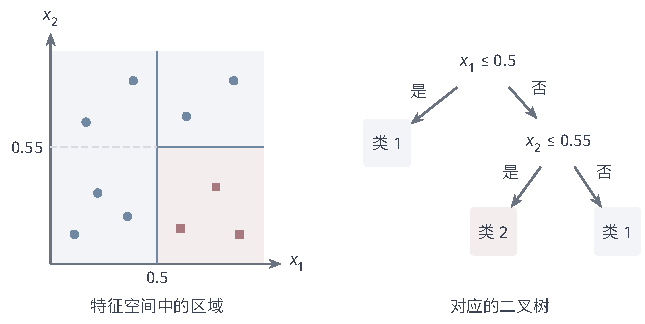
\includegraphics[width=109.241mm]{figures/04-classic-models/00-shared/tikz/classification-tree-partition/figure.pdf}
  \caption{二维分类的教学构造。左图为归一化特征空间$[0,1]^2$中的区域划分，圆点表示类1，方点表示类2；右图为产生同一划分的条件树。根节点检查$x_1\leq0.5$，仅在其“否”分支上继续检查$x_2\leq0.55$。点的位置与分裂阈值均为人为设定，不代表真实数据实验。}
  \label{fig:classification-tree-partition}
\end{figure}

不同树算法的主要差异落在三个问题上：怎样评价一次分裂，允许什么样的分支结构，怎样控制树的大小。ID3提供了信息增益驱动的基本构造，C4.5扩展其评分和数据处理方式；CART则采用统一的二叉划分与子树选择框架，形成了另一条决策树研究路线。

\subsection{ID3}
\label{sec:classification-id3}

要决定先检查哪个特征，需要比较“检查前还分不清多少类别”和“检查后还分不清多少类别”。ID3（Iterative Dichotomiser 3）据此选择特征，再在各分支上重复同一过程。Quinlan在1986年的论文中将ID3追溯到Hunt等人的概念学习系统（Concept Learning System, CLS）：CLS向前考察若干层候选树，按测量与误分类代价选择测试；ID3则改用信息驱动的局部评价。这一变化把建树中的“先测什么”落实为当前节点上可计算的信息增益比较，优化范围限定在当前节点的候选测试。本节采用以离散特征、信息增益和不作后剪枝为设定的基本ID3\scite{quinlan1986trees}。

\subsubsection{模型结构}
\label{sec:classification-id3-structure}

在节点样本集$D$上，记$p_c(D)$为类别$c$的样本比例。\term{熵}（entropy）用一个数概括类别分布的不确定性：节点只含一类时为零，各类越均匀，熵越大。采用以2为底的对数，
\begin{equation}
  H(D)=-\sum_{c=1}^{C}p_c(D)\log_2 p_c(D),
  \label{eq:classification-entropy}
\end{equation}
其中约定$0\log_2 0=0$。对第$j$个离散特征，令$V_j$为其可能取值集合，$D_{j,v}=\{(\bm{x}_i,y_i)\in D:x_{i,j}=v\}$。该特征的\term{信息增益}（information gain）是分裂前后熵的减少量：
\begin{equation}
  \operatorname{Gain}(D,j)
  =H(D)-\sum_{v\in V_j}\frac{|D_{j,v}|}{|D|}H(D_{j,v}).
  \label{eq:classification-information-gain}
\end{equation}
空子集对求和的贡献定义为零。这里必须按子集大小加权，否则只有一个样本的小分支会与包含大部分样本的分支同样重要。

ID3用选中的特征建立一个内部节点，每个取值对应一个分支。叶节点保存到达该处的类别计数，并通常输出多数类；类别计数相同时使用预先固定的平局规则。这样得到的是分段常值分类器：同一叶区域内的所有输入具有相同预测。叶节点也可报告类别频率，但少量样本上的频率不应被直接理解为可靠的概率估计。

信息增益把分裂选择变成了可计算的局部比较，却有\term{多值偏差}（multivalued attribute bias）：取值很多的特征更容易把训练样本分成纯净的小组。若每条记录的编号都不同，用编号分裂会使所有子节点熵为零，增益达到$H(D)$，但对一个新编号几乎没有帮助。

\subsubsection{参数学习}
\label{sec:classification-id3-learning}

从根节点的$D_n$出发，算法计算所有可用特征的信息增益，选择最大者，再分别对其子集递归建树。离散特征已经按取值完全展开后，同一路径上不必再次使用它。若当前样本全部同类，就生成该类叶节点；若可用特征耗尽而标签仍不一致，就输出当前多数类。对训练时未出现的分支，可以保留以父节点多数类为输出的回退叶节点，使预测规则对新输入仍有定义。

每次选择只依据当前节点，因而这是\term{贪心搜索}（greedy search）：接受眼前收益最大的分裂，不回头枚举所有可能的整棵树。基本ID3不在建树后再作剪枝；限制最大深度、最小叶样本数或最小增益，属于另外加入的生长控制。尤其是“增益为零就停止”也会改变基本搜索行为：在异或关系中，单个特征的增益可能为零，而连续两次测试可以完全分开类别。停止规则既能减少无效分裂，也可能阻止发现特征交互。

\subsubsection{理论分析}

\paragraph{表达能力}
对有限取值特征，若允许一条路径检查全部$d$个特征、保留至多$\prod_j|V_j|$个叶，就能为每个取值组合单独指定类别。因此任意只依赖这些字段的确定性类别映射都在这个树类中；有标签噪声时，完整组合上的类别分布也可由相应叶的概率向量表示。逐层组合坐标条件使树能够表示高阶交互。例如四点异或只需先检查$x_1$、再在两个分支分别检查$x_2$，深度为2、叶数为4；一层树却只能按一个坐标分组，在等概率四点上至少有一半标签无法吻合。

一旦限制深度或合并叶，尚未区分的取值组合就必须共用预测。这个限制不能靠增加同类样本消除。同一份特征记录若对应不同标签，树也无法逐条区分，只能用类别分布或多数类概括该处的随机性。



\paragraph{收敛性}
离散特征在同一路径最多使用一次，因此树深度至多为$d$，递归必然停止。每层所有非空节点合计处理至多$n$条记录；按每个节点扫描剩余字段的直接实现，建树成本至多为$O(nd^2)$，不计显式列出未观测空分支的成本。有限树类中的最小训练错误一定存在，但逐节点最大化信息增益并不求解这个全局问题，不能把递归结束理解为找到了训练错误最小的树。

\paragraph{泛化性}
\begin{theorem}[ID3在有限离散输入下的期望分类风险界]
固定各字段的有限取值集合，令$V=\prod_j|V_j|$。完整输入组合上的确定性分类器至多有$C^V$个；ID3返回的树，无论如何选择分裂，都属于这个固定集合。由式\eqref{eq:regression-finite-class-deviation}，对$n$个独立同分布的训练样本，以至少$1-\delta$的概率，
\[
 R_{01}(\hat h)\leq\widehat R_{01}(\hat h)
       +\sqrt{\frac{V\log C+\log(2/\delta)}{2n}}.
\]
\end{theorem}

这个界直接覆盖由训练数据选出的树，却可能因输入组合太多而没有实用精度。限制树的规模可以缩小候选数；未预先限定的新类别取值或连续阈值不满足这里的有限输入假设。

\subsubsection{优化泛化能力}

若关注的不只是类别变纯，还包括分裂是否有足够的统计证据，可以采用Kass于1980年提出的\term{卡方自动交互检测}（chi-square automatic interaction detection, CHAID）。它对类别特征的取值与标签建立列联表，先合并类别分布差异不显著的取值，再比较各特征与响应的关联，按经过多重比较调整的检验结果选择分裂；证据不足时停止。剩下的取值组形成多路分支，适合把分群结果读作交叉分类，但连续变量通常需要先分组，分组方式会影响结果。检验显著性针对相应的关联原假设，树的预测误差还需另行评价\scite{kass1980chaid}。

\subsubsection{小结}
\label{sec:classification-id3-summary}

ID3把离散字段逐层组织为类别区域，用当前节点的信息增益决定下一次测试。取值很多的字段容易获得较高增益，训练噪声也可能被写成细小分支。关联检验提供了另一种控制生长的依据，C4.5则继续调整评分和数据处理；应区分测试能表达什么与搜索为何选择它。

\subsection{C4.5}
\label{sec:classification-c45}

ID3的基本构造已经能从离散特征递归建树，但前面用记录编号的例子说明，信息增益会偏爱把训练样本切得很细的特征。实际记录还常有连续测量值和缺失字段：不能为每个长度值都建立一条新分支，也不能遇到未知值就让预测失去定义。让树处理这些数据，需要同时调整测试评分、阈值选择与缺失记录的传递方式。

Quinlan在1993年的专著中给出了C4.5的完整程序体系。它沿用ID3的递归构造，用增益率抑制部分多值偏差，通过阈值测试处理连续变量，并以分数权重传递缺失记录；树长成以后，再用错误估计剪枝和规则提取控制结构。以下分别说明这些机制如何工作\scite{quinlan1993c45}。

\subsubsection{模型结构}
\label{sec:classification-c45-structure}

多值特征容易得到大增益，是因为它本身就把数据切得很细。C4.5用\term{信息增益率}（gain ratio）比较“类别信息的增加”与“产生这些分支所需的划分信息”。设测试$a$把$D$分成$D_1,\ldots,D_b$，令$q_v=|D_v|/|D|$，则
\begin{align}
  \operatorname{SplitInfo}(D,a)
  &=-\sum_{v=1}^{b}q_v\log_2 q_v,
  \label{eq:classification-split-information}\\
  \operatorname{GainRatio}(D,a)
  &=\frac{\operatorname{Gain}(D,a)}
  {\operatorname{SplitInfo}(D,a)}.
  \label{eq:classification-gain-ratio}
\end{align}
这里的信息增益仍按式\eqref{eq:classification-information-gain}计算，只把按特征取值划分替换为测试$a$的各个结果。分母为零意味着没有真正划分，不能参与比值比较。

小分母会改变增益率的排序：只分离少量样本的测试具有较小的划分信息，微小信息增益也可能得到较大比值。C4.5先计算候选的平均信息增益，再在增益不低于平均值的测试中比较增益率。这个启发式筛选限制依靠小分母取胜的候选，实际预测价值仍由独立验证评价。

\subsubsection{参数学习}
\label{sec:classification-c45-learning}

离散特征可以按取值作多路分裂；连续特征则使用$x_j\leq t$与$x_j>t$的二路测试。候选阈值来自排序后相邻不同取值之间，且分裂后必须满足最小子节点样本量等限制。连续特征在某次分裂后仍可在后代节点使用，因为同一数值轴上可能需要多个阈值。

C4.5各版本对阈值的评价略有区别。较早版本按增益率选择阈值；Quinlan在1996年的修订中先按信息增益选择连续特征的阈值，再扣除搜索阈值所需的描述长度代价，参与特征之间的增益筛选和增益率比较。若有$q$个候选切分位置，这项逐样本惩罚形如$\log_2 q/|D|$，用来抵消“可试阈值更多”带来的选择优势。算法~\ref{alg:classification-c45}突出这些版本共有的建树骨架，把阈值评价留在候选测试生成步骤中\scite{quinlan1996continuous}。

\begin{algorithm}[C4.5的递归生长与后剪枝]
  \label{alg:classification-c45}
  \begin{algorithmic}[1]
    \Require 节点样本$D$，可用特征集合$F$，停止及剪枝设置
    \Ensure 剪枝后的分类树
    \Function{Grow}{$D,F$}
      \If{$D$全部同类，或样本量不足，或$F$为空}
        \State \Return 以$D$中多数类为输出的叶节点
      \EndIf
      \State 生成各特征的有效测试，连续特征同时选择阈值
      \State 计算各测试的增益；缺失值按正文约定处理
      \If{没有有效测试，或最大增益不为正}
        \State \Return 以$D$中多数类为输出的叶节点
      \EndIf
      \State 求候选测试的平均增益$\bar g$
      \State 保留增益不低于$\bar g$且划分信息为正的测试
      \State 选择其中增益率最大的测试$a$，建立节点$T$
      \For{测试$a$的每个结果$v$}
        \State 得到相应的子集$D_v$及子问题的特征集合$F_v$
        \If{$D_v$为空}
          \State 将$D$的多数类叶节点接到分支$v$
        \Else
          \State 将$\Call{Grow}{D_v,F_v}$接到分支$v$
        \EndIf
      \EndFor
      \State \Return $T$
    \EndFunction
    \State $T\gets\Call{Grow}{D,F}$
    \State 自底向上比较子树与简化方案的悲观错误估计
    \State \Return 剪枝后的$T$
  \end{algorithmic}
\end{algorithm}

缺失值需要在评分和路由中保留不确定性。设测试$a$的已知样本总权重占当前节点的比例为$q_{\mathrm{known}}$，C4.5在已知样本上估计熵下降，再乘$q_{\mathrm{known}}$降低该测试的收益；划分信息也计入未知部分。选择测试后，缺失记录按已知样本进入各分支的比例作分数权重分配，后续熵、类别计数和多数类都使用这些权重。预测遇到缺失值时，也按分支权重综合子树输出。

树生长完成后，C4.5采用\term{悲观错误剪枝}（pessimistic error pruning）：训练误差倾向于低估新样本错误，因而以二项错误计数的上置信估计作修正，比较保留子树与折叠成多数类叶节点的估计错误数。若简化方案不更差，就可以删除该子树；完整实现还可考察用某个子树提升替代当前分支。置信设置控制剪枝强度，这一自适应建树后的估计用于启发式模型选择，整树的样本外错误仍通过验证或测试数据评价。

树也可以转成规则：每条根到叶路径的测试构成规则前件，叶类别作为后件，再尝试删除不必要条件并筛选规则。未经简化的路径规则继承树的区域划分；条件删除以后可能产生重叠，因此规则系统还必须规定冲突处理和默认预测。这种转换并非只把树的文字抄成一份无序清单。

\subsubsection{理论分析}

\paragraph{表达能力}
连续特征的单坐标阈值把每个叶区域限制为坐标区间的交，也就是轴对齐的矩形或更高维的长方体。几个这样的区域可以精确表达前面的分段教学规则，却不能用有限条轴对齐边界精确重现整条斜线。表示限制在于分区方向，增益率只改变选择哪次分裂。

这个差距可以随着树的规模减小。例如，设输入在$[0,1]^2$上均匀分布，真实类别由$x_2>x_1$决定。把$x_1$轴等分为$m$个宽度$1/m$的区间，在每个区间内以其中点作为$x_2$阈值，至多$2m$个叶就能形成阶梯边界。每个竖条内与目标不一致的面积为$1/(4m^2)$，合计为$1/(4m)$。因此，至多$2m$叶的候选族中存在一个标签不一致比例为$1/(4m)$的表示。缺失字段的输入则没有提供该坐标的真实值；若两个对象的已观测字段相同，仅依赖这些字段的候选无法区分它们。



\paragraph{收敛性}
对完整输入，合法分裂将节点中的样本分为至少两个非空子集，沿任一路径的样本数严格减少，故至多$n$个非空叶后生长结束。缺失记录按权重分流时，不能继续用这条整数计数证明；实现需明确最小有效样本量，并可用预定最大深度保证有限终止。剪枝对有限树作有限次替换，同样会结束。增益率与局部错误估计都不是整棵树训练目标的精确求解器，因此没有由这些步骤自动推出的全局最优收敛率。

\paragraph{泛化性}
\begin{theorem}[C4.5冻结候选树在独立验证下的期望风险界]
连续阈值由训练数据确定，缺失输入还可能混合多个分支，因而不能只数最终树上出现的阈值来控制训练偏差。可以先用生长数据生成$J$棵完整预测规则固定的候选树，再在独立的$m$个同分布验证样本上选择错误率最小的$\hat h$。条件于这些候选树，零一损失的Hoeffding界与并集界给出，以至少$1-\delta$的概率，
\[
 R_{01}(\hat h)\leq\min_{1\leq j\leq J}R_{01}(h_j)
            +2\sqrt{\frac{\log(2J/\delta)}{2m}}.
\]
\end{theorem}

前一项保留候选树本身的质量，后一项控制验证选择的误差。该结论适用于这一独立验证协议，不能替换为C4.5内部的悲观错误估计；反复读取同一验证集来生成新树也不满足冻结候选的条件。

\subsubsection{优化泛化能力}

来自不同抽样来源的记录，未必应有相同训练权重。C4.5之后的C5.0加入了样本权重、误分类代价和特征筛选等功能\scite{rulequest2017c50}。样本权重调节不同记录在拟合中的贡献，让树与规则的选择更接近所关注的数据分布。权重需要有相应的抽样或评价依据；任意放大某些记录的贡献并不保证降低总体风险。

\subsubsection{优化计算能力}

数据规模增加时，树或规则生成过程的时间与内存也会限制使用。C5.0在C4.5之后继续改进这些实现；RuleQuest提供商业版本和GPL源码版本，其公开实验报告了特定数据与硬件条件下的速度及内存改进\scite{rulequest2017c50}。比较时应固定数据、硬件和输出形式，因为生成树与生成规则集的开销可以不同。实现上的节省与误分类代价设置处理的是不同问题，需要分别记录资源消耗和分类错误。

\subsubsection{支持误分类代价不同的场景}

邮件过滤中，误拦一封正常邮件与漏放一封垃圾邮件可能具有不同代价。误分类代价把这种差异写入损失，使树与规则按所关心的错误代价评分和选择。这里扩展的是评价目标，预测仍使用相应的树或规则表示。

\subsubsection{小结}
\label{sec:classification-c45-summary}

C4.5在ID3式递归划分中补充分裂评分、连续阈值、缺失字段传递与后剪枝，并可把路径转成规则。它处理的困难不只是分裂后类别是否更纯，还包括记录怎样经过分支，以及长成的树应保留多少细节。

C5.0继续改善树与规则生成，并使训练能够考虑样本权重和误判代价。实现效率与实际决策中的错误成本因而进入选择，但仍应检查所用字段是否有意义、缺失值如何影响预测，以及最终条件能否被审阅。

\subsection{CART}
\label{sec:classification-cart}

另一种组织树的方法是把每次测试都限定成二选一，再统一研究大树中应保留哪些子树。\term{分类与回归树}（classification and regression trees, CART）采用这一框架；Breiman、Friedman、Olshen与Stone在1984年的专著中将树的构造、最优剪枝与统计性质放在同一体系中讨论。其中，代价复杂度剪枝把“怎样长出一棵大树”与“最终保留多大的子树”分开：生长阶段比较局部分裂，剪枝阶段形成候选子树序列，再用验证选择规模。因此，CART与ID3的区别不只是换一个不纯度指标，还涉及分支结构与整树选择。这里关注分类树；第\ref{sec:regression-cart}节的回归CART复用递归二分与代价复杂度剪枝，但按响应损失选择分裂并在叶内输出数值，本节则按类别不纯度或误分类代价分裂并输出类别标签或类别比例\scite{breiman1984cart}。

\subsubsection{模型结构}
\label{sec:classification-cart-structure}

CART分类树通常用\term{基尼不纯度}（Gini impurity）评价节点中类别的混杂程度：
\begin{equation}
  G(D)=1-\sum_{c=1}^{C}p_c(D)^2.
  \label{eq:classification-gini}
\end{equation}
它也等于从节点经验类别分布独立抽取两个标签时，两者不同的概率。对于产生左右子集$D_{\mathrm{L}}$和$D_{\mathrm{R}}$的测试$a$，比较
\begin{equation}
  \Delta G(D,a)=G(D)
  -\sum_{v\in\{\mathrm{L},\mathrm{R}\}}
  \frac{|D_v|}{|D|}G(D_v).
  \label{eq:classification-gini-decrease}
\end{equation}
基尼与熵都鼓励子节点变纯，但并不总给出相同的排序。基尼计算省去对数运算，整棵树的训练成本还包含阈值搜索与数据访问。

对连续特征，二分测试仍是阈值比较；对类别特征，测试可写成$x_j\in S$与$x_j\notin S$，其中$S$是部分取值组成的集合。寻找这个集合本身也是搜索问题，候选分组数随取值数增加，搜索成本需要计入建树预算。统一的二叉结构便于遍历和剪枝，但可能用多层测试表达一棵多路树的一次分裂。

\subsubsection{参数学习}
\label{sec:classification-cart-learning}

生长阶段反复选择基尼下降最大的有效二分测试，直到满足生长限制，得到一棵较大的树$T_0$。随后进行\term{代价复杂度剪枝}（cost-complexity pruning）：不再逐个比较局部增益，而是在$T_0$的候选子树中平衡拟合误差和叶节点数。令$L(T)$为树$T$的叶节点集合，$\hat c_\ell$为叶$\ell$的预测类别，定义
\begin{align}
  \widehat R(T)
  &=\frac{1}{n}\sum_{\ell\in L(T)}
    \sum_{(\bm{x}_i,y_i)\in D_\ell}
    \mathbb{1}\{y_i\neq\hat c_\ell\},
  \label{eq:classification-cart-empirical-risk}\\
  J_\alpha(T)&=\widehat R(T)+\alpha|L(T)|,
  \qquad \alpha\geq0.
  \label{eq:classification-cart-cost-complexity}
\end{align}
这里$\widehat R(T)$采用全训练集上的误分类比例，使不同子树的误差具有共同尺度。有些软件把叶不纯度的加权和作为剪枝代价；使用其参数时需要核对具体定义，再按该尺度解释$\alpha$。

剪枝路径可以由\term{最弱环节剪枝}（weakest-link pruning）生成。设内部节点$t$以下的子树为$T_t$，把它折叠成一个叶节点后，该区域对全训练集误差的贡献为$\widehat R(t)$；保留时贡献为$\widehat R(T_t)$。两种方案的代价相等时，
\begin{equation}
  \alpha_t=
  \frac{\widehat R(t)-\widehat R(T_t)}
       {|L(T_t)|-1}.
  \label{eq:classification-weakest-link}
\end{equation}
分子是折叠后增加的训练错误，分母是删去的叶数，因而$\alpha_t$衡量“每少保留一个叶节点要付出多少误差”。剪去最小$\alpha_t$对应的分支，再重新计算，就得到从大树到根叶节点的嵌套序列。若某些分支增加叶数却不降低误分类率，可先在$\alpha=0$时合并；临界值处可能有多个最优子树，按一致的最小子树约定处理平局。

对每个$\alpha$，上述序列包含相应的最优剪枝子树，最优性范围限定为给定$T_0$的剪枝子树。实际需要用验证集或交叉验证选择$\alpha$；交叉验证时，在各训练折内独立生长和剪枝，再评价对应验证折。

预测还要规定主测试字段缺失时如何分支。CART的\term{替代分裂}（surrogate split）寻找其他特征测试，按它们复现主分裂结果的程度选择替代；类别权重和误分类代价也可以改变生长与叶预测。具体实现采用哪些机制，需要与数据处理方式一同检查。

\subsubsection{理论分析}
\label{sec:classification-cart-theory}

\paragraph{表达能力}
CART与完整输入上的C4.5共享单坐标阈值的矩形分区能力，前面$2m$个叶、错误率$1/(4m)$的斜线逼近也可由二叉树实现。有限离散输入上的任意取值映射同样可以逐次二分展开，但叶数必须足以区分所需组合。二叉与多路的区别主要影响树深和条件复用，并不使基尼评分获得一种新的边界形状。

测试全集还会留下独立于叶数的限制。若两个输入对全部允许测试都给出相同结果，无论树怎样增长，它们都会走到同一叶，必须得到相同类别。测试集合固定时，增加叶数只能细化已允许的测试组合；目标所需的阈值或特征不在测试集合中时，逼近差距仍然存在。



\paragraph{收敛性}
在无缺失、每次产生两个非空子节点的设定下，生长至多产生$n$个非空叶。成本复杂度剪枝从这棵有限大树出发，每次减少内部节点，剪枝路径也有限。对固定叶数上限和有限测试集，全局最优树存在；但贪心生长不保证找到它。剪枝的最优性只针对给定大树的子树，不能扩展为所有可构造树的最优性。

\paragraph{泛化性}
节点类别变纯，是当前训练子集上的变化；要控制整棵树在新样本上的错误，还要把选测试、选结构和选叶标签造成的选择范围计入。先考虑一个明确受限的版本：输入没有缺失，抽样前给定有限测试集合，并限制最多保留多少个叶节点。
\begin{theorem}[CART在固定测试集与叶数约束下的期望分类风险界]
  \label{thm:classification-tree-risk}
  设训练样本独立同分布，类别数为$C\geq2$。抽样前固定$Q\geq1$个二值测试和叶数上限$L\geq1$；候选类$\mathcal T_{Q,L}$包含用这些测试构造、至多$L$个叶、各叶输出一个类别的所有二叉树。令
  \[
    u_{\mathrm T}=
      \sqrt{\frac{\log(2L/\delta)
        +(L-1)\log(4Q)+L\log C}{2n}},
       \qquad0<\delta<1.
  \]
  CART学习器通过生长与剪枝返回$\hat T\in\mathcal T_{Q,L}$。至少以$1-\delta$的概率，
  \[
    R_{01}(\hat T)
      \leq\widehat R(\hat T)+u_{\mathrm T}.
  \]
  在同一事件上，若
  $e_{\mathrm{opt}}=\widehat R(\hat T)
      -\min_{T\in\mathcal T_{Q,L}}\widehat R(T)$，则
  \[
    R_{01}(\hat T)-R^\ast
      \leq\inf_{T\in\mathcal T_{Q,L}}R_{01}(T)-R^\ast
            +2u_{\mathrm T}+e_{\mathrm{opt}}.
  \]
\end{theorem}
\begin{proof}
  有$\ell$个叶的有序满二叉树形状数为第$\ell-1$个Catalan数，至多$4^{\ell-1}$。每个内部节点有$Q$种测试，每个叶有$C$种输出，所以
  \[
    |\mathcal T_{Q,L}|
       \leq\sum_{\ell=1}^L4^{\ell-1}Q^{\ell-1}C^\ell
       \leq L(4Q)^{L-1}C^L.
  \]
  零一损失位于$[0,1]$，对这个预定有限类应用式\eqref{eq:regression-finite-class-deviation}的一致偏差界，便得$u_{\mathrm T}$。该事件同时覆盖全部候选树，因此也覆盖依训练数据选出的$\hat T$。用它先比较$R_{01}(\hat T)$与$\widehat R(\hat T)$，再加上$e_{\mathrm{opt}}$并与任意候选树比较，最后把候选树的经验风险换回期望风险，即得第二个结论。
\end{proof}

这里不要求CART找到所有树中的经验最优解；贪心生长和给定大树内的最优剪枝，未必使$e_{\mathrm{opt}}$为零。第一个界对任意返回的受限树成立，第二个界则保留它与候选类经验最优者的搜索差距。叶数增多可能减小逼近差距，却同时增大抽样误差项。

在完整的有限类别输入上，ID3与C4.5的多路测试也可以展开为若干二值测试；若测试全集和叶数上限预先固定，展开后的树满足同一个结论。通常实现从训练数值中挑选连续阈值，或对缺失输入混合分支预测，这些情形没有自动满足上述有限类假设。尤其不能在建树之后，把实际考察过的测试数当作预定的$Q$。若对独立验证集上的一条预先生成剪枝路径选择子树，可以条件于生长数据，再按候选子树数控制验证选择；其风险依据来自验证抽样，而不是节点不纯度本身。

\subsubsection{优化表达能力}

常数叶用一个概率向量概括区域中的全部输入；若同一区域内的概率仍随特征变化，可以保留树的划分，改变叶节点如何预测。\term{逻辑模型树}（logistic model tree, LMT）在每个叶区域内使用Logistic回归，即用特征的线性得分表示类别对数几率，再转成类别概率。这样，树负责不同区域之间的结构变化，叶模型负责区域内部随特征变化的概率。Landwehr、Hall与Frank的2005年期刊论文基于其2003年会议工作，结合C4.5分裂与CART剪枝形成树结构，并通过LogitBoost逐步拟合逻辑模型。在后代节点继续细化祖先模型，可以避免每个小叶都从零估计全部系数\scite{landwehr2005lmt}。

例如在二分类叶区域$\ell$内，LMT可输出
\begin{equation}
  \hat p_\ell(y=1\mid\bm{x})
  =\frac{1}{1+\exp[-(\bm{w}_\ell^\top\bm{x}+b_\ell)]},
  \label{eq:classification-lmt-leaf}
\end{equation}
其中$\bm{w}_\ell\in\mathbb{R}^d$和$b_\ell\in\mathbb{R}$是叶模型的系数。概率在单个叶区域内部平滑变化，但跨越不同叶的边界时仍可能跳变，也不自动具有良好的校准性质。模型拟合、迭代次数选择和树剪枝共同增加训练成本，解释时也要同时阅读路径条件与叶模型系数。
LMT能精确表达“各叶区域内对数几率分别为仿射函数”的后验，只要树能够形成这些区域。普通常值叶只能用一个概率概括叶内全部输入；LMT可以保留其中的线性变化，却仍不能在具有非零长度的连续输入区间内精确表达$x^2$这样的对数几率。进一步划分区域能够改善逼近，不能免除叶数与样本覆盖的限制。

\subsubsection{优化泛化能力}

信息增益和基尼下降还面临另一种偏差：候选切分越多，越容易偶然找到一个高分切分。\term{条件推断树}（conditional inference tree, CTree）把“选哪个特征”与“在该特征上怎样切分”分开。Hothorn、Hornik与Zeileis在2006年的框架中用条件置换分布评价特征与响应的关联：先检验当前节点中所有特征均与响应无关联的全局原假设；不能拒绝时停止，否则选择检验证据最强的特征，再为它寻找二分位置。通过同一检验尺度和多重检验控制，可以缓解不同取值数目带来的选择偏差\scite{hothorn2006ctree}。

CTree的置换检验依赖原假设下的可交换性，渐近近似的精度也受样本量影响。检验控制当前节点是否继续分裂，全树的预测质量仍应在独立数据上评价。

检验驱动的生长也有搜索边界：四点异或在两层树中可被精确表示，但根节点的每个单坐标都与标签独立，单变量检验可能阻止继续分裂。检验决定当前节点是否继续搜索，并不改变候选树本来能够表示的关系。

\subsubsection{小结}
\label{sec:classification-cart-summary}

把叶节点多数类换成数值均值，把分类不纯度换成平方误差，就得到平方损失下的回归树构造；不需要另换一种树的表示。多个树怎样组合，见第\ref{chap:ensemble-learning}章。

CART把二叉分裂的局部选择与整树规模的验证选择分开。条件推断树采用另一种分裂依据，先比较特征与类别的关联，再确定切分位置；这种选择针对候选切分数影响评分的问题。

若常数叶遗漏区域内部的概率变化，逻辑模型树可以在叶内使用特征得分，并结合C4.5分裂与CART剪枝组织区域。代价是还要拟合和选择叶模型，解释时同时阅读路径与系数。分裂选择、树的规模和叶内预测各处理不同困难，类别不平衡、缺失字段与误判代价也须在对应机制中处理。

\subsection{规则分类与RIPPER}
\label{sec:classification-rules}
\label{sec:classification-ripper}

一棵树把全部输入组织成从根出发的路径，规则列表则可以直接列出若干足以作出类别判断的条件。例如，目标类若由几个分离的小区域组成，我们可以分别为这些区域学习短规则，而不要求它们共享同一个根测试。规则简化后还可能重叠，因而需要约定命中多条规则时怎样预测。第\ref{sec:classic-overview-tree-rules}节已介绍这种表示差别；这里采用有序规则，按首次命中的结论判类，没有命中时使用默认类。

逐条学习规则时，一个直接困难是：为了覆盖少量例外，不断增加条件会产生庞大的规则集；过早删去条件，又可能丢失有用的局部结构。早期的AQ系列探索了从样本归纳条件规则的路线，后来的规则学习把覆盖策略与误差控制结合起来。Fürnkranz与Widmer在1994年提出\term{增量减错剪枝}（incremental reduced error pruning, IREP），将单条规则的增长和立即剪枝嵌入逐条学习过程，以避免先生成庞大规则集再统一简化的开销\scite{furnkranz1994irep}。

Cohen在1995年改进IREP的剪枝评分和停止准则，并加入整组规则的反复优化，形成RIPPER（Repeated Incremental Pruning to Produce Error Reduction）。RIPPER通过规则增长、留出剪枝、顺序覆盖和整组优化，在长度、覆盖范围与错误之间实施启发式搜索。下面分解这些步骤\scite{cohen1995ripper}。

\subsubsection{模型结构}
\label{sec:classification-ripper-structure}

RIPPER输出有序规则以及一个默认类别$c_0$。第$r$条规则的前件可写为
\begin{equation}
  a_r(\bm{x})=\bigwedge_{j=1}^{m_r}b_{r,j}(\bm{x}),
  \qquad a_r(\bm{x})\Longrightarrow y=c_r,
  \label{eq:classification-rule-form}
\end{equation}
其中$b_{r,j}$是一个返回真或假的测试，$m_r$为该规则的条件数。例如，$x_1>60$与$x_2=\text{是}$可以组成一个合取，但每个测试的业务含义必须由特征定义决定。规则\term{覆盖}（cover）样本，指样本满足其前件，与样本真实标签是否等于后件无关。

若规则数为$s$，预测时寻找最小的$r\in\{1,\ldots,s\}$使$a_r(\bm{x})$成立，输出$c_r$；不存在这样的$r$时输出$c_0$。二分类中，可以为目标类学习若干规则，把另一类作为默认类。多分类时，经典RIPPER通常按类别出现频率由低到高学习，逐次区分当前类与尚待区分的其他类，把最常见类放在默认位置。这种类别排序有助于为少数类显式生成规则，但不构成少数类召回率的保证。

\subsubsection{参数学习}
\label{sec:classification-ripper-learning}

RIPPER采用\term{顺序覆盖}（sequential covering），这个名字描述了规则逐条“占领地盘”的过程：每次只在还没有被任何规则覆盖的样本上学习一条规则，把它加到有序列表的末尾，然后把它命中的样本从工作集中拿走，再对剩下的样本学习下一条；如此反复，直到没有目标类样本剩下。需要强调的是，被一条规则误覆盖的负例虽然从“找下一条规则”的工作集中移除，但在给整组规则打分时仍然计入，因此一条乱覆盖负例的规则不会因为样本被移走就逃避惩罚。设当前目标类别为$c_+$，属于该类的记录称为正例，其余为负例。保留原始二类训练集$D^{(0)}$用于整体评分，另用$U$表示不断缩小的覆盖工作集。从$U$移除的误覆盖负例仍保留在$D^{(0)}$中，并计入整体错误。

学习单条规则时，先分层随机划分增长集与剪枝集，经典设置约为$2:1$。增长从空前件开始，空前件覆盖所有样本；每次添加一个测试，使前件更严格、覆盖范围更小。测试可直接使用连续特征的阈值，无须一律在训练前离散化。Cohen的实现对缺失特征采用保守约定：涉及该特征的测试在缺失记录上不成立，因此规则需要其他已知字段来覆盖这些记录。

增长时使用源自FOIL（First Order Inductive Learner）的信息增益评分。设加入条件前覆盖$p_0$个正例、$q_0$个负例，加入后覆盖$p_1$个正例、$q_1$个负例，其中$q$不表示全章的样本量$n$。在命题规则设定下，评分为
\begin{equation}
  g=p_1\left(
  \log_2\frac{p_1}{p_1+q_1}
  -\log_2\frac{p_0}{p_0+q_0}
  \right).
  \label{eq:classification-foil-gain}
\end{equation}
括号比较加入条件前后的正例纯度，外面的$p_1$避免只看纯度而忽略保留下来的正例数。候选条件必须保留正例并满足覆盖量等实现约束；增长通常持续到不再覆盖增长集负例，或没有可接受的改进条件。噪声样本可能使负例始终被覆盖，此时由可接受条件和覆盖约束结束增长。

剪枝则允许把规则末端的一串条件一起删掉，也就是比较增长过程中得到的各个前缀，而非只尝试删去一个条件。若某个前缀在剪枝集覆盖$p$个正例、$q$个负例，RIPPER的基本评分是
\begin{equation}
  v=\frac{p-q}{p+q},\qquad p+q>0.
  \label{eq:classification-ripper-pruning}
\end{equation}
在分母为正时，它与覆盖样本中的正确率$p/(p+q)$给出相同排序。剪枝选择评分最好的可接受前缀，平局可偏向较短者；覆盖不到剪枝样本时，分数未定义，需执行预先规定的回退或拒绝规则。这一评分改变了原IREP对规则的偏好，尤其避免单凭覆盖大量样本而认可纯度不足的条件。

单条规则看起来合理，也可能使整组规则过于复杂。\term{最小描述长度}（minimum description length, MDL）把这种取舍表达为：用多少比特写下规则，再用多少比特说明规则预测错了哪些训练标签。记有序规则集为$\mathcal{R}$，总描述长度可概括为
\begin{equation}
  L_{\mathrm{total}}(\mathcal{R};D^{(0)})
  =L_{\mathrm{rules}}(\mathcal{R})
   +L_{\mathrm{errors}}(D^{(0)}\mid\mathcal{R}).
  \label{eq:classification-rule-description-length}
\end{equation}
第二项按完整规则集及默认类计算，因而仍包含误覆盖记录。Cohen的实验允许总长度暂时超过此前的最小值，但超过64比特就停止增加规则，再从后向前删除会增加总长度的规则。64比特是该实现允许暂时增加描述长度的预算；规则增加后统一按总长度检查停止和删除。

算法~\ref{alg:classification-ripper}给出二类子问题的主要流程。伪代码中的增长和剪枝采用前述评分，描述长度的编码细节由具体实现确定；多分类时在外层加入类别排序与默认类约定。

\begin{algorithm}[RIPPER的覆盖学习与规则优化]
  \label{alg:classification-ripper}
  \begin{algorithmic}[1]
    \Require 二类样本$D^{(0)}$，目标类$c_+$，优化轮数$b$
    \Ensure 有序规则集$\mathcal{R}$及默认负类
    \State $\mathcal{R}\gets()$
    \Function{Extend}{$\mathcal{R},D^{(0)}$}
      \State $U\gets D^{(0)}$中未被$\mathcal{R}$覆盖的样本
      \State $L_{\min}\gets L_{\mathrm{total}}(\mathcal{R};D^{(0)})$
      \While{$U$中仍有正例}
        \State 将$U$分层随机划为增长集$G$和剪枝集$P$
        \State 从空前件增长规则$a$，按式\eqref{eq:classification-foil-gain}添加条件
        \State 在$P$上按式\eqref{eq:classification-ripper-pruning}选择$a$的前缀
        \If{无可接受规则，或$a$不覆盖$U$中的任何正例}
          \State \textbf{停止本轮覆盖学习}
        \EndIf
        \State 把$a\Longrightarrow c_+$追加到$\mathcal{R}$
        \State $L\gets L_{\mathrm{total}}(\mathcal{R};D^{(0)})$
        \State $L_{\min}\gets\min(L_{\min},L)$
        \If{$L>L_{\min}+64$}
          \State \textbf{停止本轮覆盖学习}
        \EndIf
        \State 从$U$移除被$a$覆盖的全部样本，包括正例和负例
      \EndWhile
      \State 从后向前删除能使总描述长度降低的规则
      \State \Return $\mathcal{R}$
    \EndFunction
    \State $\mathcal{R}\gets\Call{Extend}{\mathcal{R},D^{(0)}}$
    \For{$t=1,\ldots,b$}
      \For{按顺序考察$\mathcal{R}$中的每条规则}
        \State 从空前件生成替代规则，从原前件生成修订规则
        \State 剪枝候选规则时，评价完整规则集在剪枝集上的错误
        \State 用总描述长度在原规则、替代规则、修订规则之间选择
      \EndFor
      \State $\mathcal{R}\gets\Call{Extend}{\mathcal{R},D^{(0)}}$
    \EndFor
    \State \Return $\mathcal{R}$，无规则匹配时预测负类
  \end{algorithmic}
\end{algorithm}

优化阶段是在整组规则的上下文中改写单条规则。替代规则从空前件重新增长，修订规则在原前件上继续添加条件；对候选规则的剪枝不只看它自身的纯度，还看替换后完整有序规则集的错误。随后用MDL选择保留原规则还是采用候选，必要时重新进行规则删除和剩余正例的覆盖学习。原论文把一次优化称为RIPPER，重复两次称为RIPPER2；优化次数规定搜索预算，最终返回已搜索候选中的选定规则集。

\paragraph{搜索能保证到哪里}
\label{sec:classification-ripper-theory}
规则数量和条件长度决定能拼合哪些区域，当前增长、剪枝与替换策略决定实际访问哪些候选。每条有效规则至少覆盖一个尚未移除的正例，再规定有限的条件集合、规则长度和优化轮数，便可保证搜索结束；这不意味着找到了所有规则列表中的最小训练错误或最短描述。MDL与留出剪枝都是当前搜索中的选择依据，最后仍需在独立数据上评价整组有序规则。

\subsubsection{无序规则的组合}

有序规则按首次命中决定输出，排在前面的规则会遮住后面的匹配。Clark与Boswell在1991年对CN2规则学习的改进中研究了无序规则：针对类别分别生成条件，允许多个规则共同参与预测。有序规则以首次命中解决冲突；无序规则则需要组合匹配规则的类别分布或投票权重。无序表示减少了对单一顺序的依赖，却把解释负担转移到重叠和冲突处理上，因此规则学习和预测时的聚合约定需要配套选择\scite{clark1991cn2}。
无序版本改变了重叠区域中的输出组合，不能只按有序列表理解。减少顺序依赖也不意味着预测无需约定：冲突规则怎样合并、没有规则命中时怎样回退，都属于完整的分类器。

\subsubsection{CN2的束搜索}

RIPPER增长一条规则时沿当前条件链继续搜索；若希望同时保留几条条件链，可以比较另一种规则搜索策略。Clark与Niblett在1989年提出的CN2采用这种做法，是另一条直接规则学习路线。它结合AQ的规则覆盖思想与类似ID3的纯度评价，用\term{束搜索}（beam search）寻找条件合取：每轮扩展已有候选，只保留评分最好的$b$个候选继续搜索，其中$b$为束宽。

束宽大于1时，相较于每轮只保留一条条件链的贪心搜索，束搜索可以评价更多候选，也有机会继续探索另一条暂时评分较低的路径。相较于不截断、把全部扩展都保留下来的穷举，限制束宽又能减少后续需要扩展的候选数。这里的“增加计算”与“节省计算”使用了不同的比较基准。

例如，构造一个最多增长3步的搜索，每条候选链在每一步都恰有4个可扩展条件，且不合并重复候选。单链贪心每层评价4个候选，共$4+4+4=12$个；束宽为2时，第一层评价4个并保留2个，后两层各评价8个，共$4+8+8=20$个；不截断时则评价$4+16+64=84$个。这个例子只比较指定搜索树中的候选评价次数，不代表CN2在所有任务上的运行时间比例。

候选截断仍可能丢弃通向最优规则的条件链，因此束搜索不提供全局最优保证。CN2还用显著性筛选限制偶然形成的纯净小区域\scite{clark1989cn2}。

在相同条件全集、前件长度和列表规模下，有序CN2与RIPPER拥有相同的规则表示能力。束宽增加的是可能找到好规则的搜索机会，不新增条件本身无法表达的关系。

\subsection{模型对比与总结}
\label{sec:classification-trees-comparison}
\label{sec:classification-rules-comparison}

表~\ref{tab:classification-tree-comparison}比较局部分裂与整树规模怎样确定。输入包含连续值或缺失字段时，需要检查测试和分支处理；最终条件要供人审阅时，树深、规则数与冲突处理同样影响选择。

ID3、C4.5与CART共享逐层测试的表示，但没有使用同一套搜索准则。C4.5沿用ID3式构造，调整多值特征评分，并补充连续阈值、缺失记录传递与后剪枝。CART把每次分裂统一为二分，再通过代价复杂度路径选择子树。多路测试可以展开成若干二值测试，却可能需要更多节点；因此“二叉”与“多叉”的名称不能直接决定哪个候选树更简洁。输入处理、分裂选择和整树规模都需要在相同任务下比较。

\begin{table}[htbp]
  \centering
  \small
  \begin{tabularx}{\linewidth}{@{}l*{3}{>{\RaggedRight\arraybackslash}X}@{}}
    \toprule
    方法 & 分裂评分 & 基本分支形式 & 规模控制 \\
    \midrule
    ID3 & 信息增益 & 离散取值多路分裂 & 基本版本无后剪枝 \\
    C4.5 & 增益筛选与增益率 & 离散多路、连续阈值二分 & 悲观错误估计剪枝 \\
    CART & 基尼不纯度下降 & 统一二叉分裂 & 代价复杂度路径及验证选择 \\
    \bottomrule
  \end{tabularx}
  \caption{三种决策树在基本分类设定下的比较。输入支持和停止细节随实现版本变化。}
  \label{tab:classification-tree-comparison}
\end{table}

若尚不清楚复杂条件是否必要，可以先建立只依赖一个字段的基线。Holte在1993年研究的\term{单特征规则}（one rule, OneR）为每个字段建立“取值到多数类”的映射，再选择训练错误较少的字段；“one”指一个字段，通常仍有多条取值规则。它便于检查单字段能够解释多少差异，却不能使用不同字段的交互\scite{holte1993oner}。

需要按几个离散字段直接查询类别时，可以采用\term{决策表}（decision table），把所选字段的取值组合作为键，同键记录共用一个预测。Kohavi在1995年研究了用验证误差选择字段子集的办法。查表减少了逐条匹配条件的工作，但字段组合容易稀疏，连续值的分箱和未见组合的回退都需要另行规定\scite{kohavi1995decisiontable}。

当字段取值有限、允许使用全部取值组合且不限制结构规模时，树、规则列表和决策表都能为每个组合指定类别。它们的主要差异在于怎样组织和搜索这些条件：树复用共同的测试前缀，规则可以为不同局部区域采用不同条件顺序，决策表统一使用一组字段作为键。OneR则把全部判断限制在单个字段，不能表达跨字段交互；它适合检验复杂组合是否确有必要。

结构受限或组合未被样本覆盖时，这些表示才会显出不同取舍。树的深度限制会把一些输入留在同一叶内；规则列表需要处理覆盖、顺序与默认类；决策表需要为稀疏和未见键规定回退。应据此比较独立验证误差、条件数量与预测成本，并把条件能否被审阅作为实际约束。

\section{基于概率的分类}
\label{sec:classification-probability}

第\ref{sec:classic-overview-probabilistic}节已区分直接建立条件类别概率与先描述类条件输入分布的两条路线。本节分别用Logistic回归、朴素贝叶斯和GDA说明参数估计、类别决策与概率检验。沿用训练集$D_n$，类别数为$C$、类别索引为$c$；$p$按观测类型表示概率质量函数或概率密度。LDA的共享协方差推导见第\ref{sec:classification-lda}节，这里直接在一般高斯模型族中使用该结果。

\subsection{Logistic 回归}
\label{sec:classification-logistic}

感知机与SVM用得分的正负决定类别，但有些任务还需要知道判断有多大把握。例如，把一封普通邮件误判为垃圾邮件，可能比让一封垃圾邮件进入收件箱更难接受。此时我们希望调整判为垃圾邮件的门槛，并用类别概率计算两种决定各自的预期代价。分类得分可以另行校准为概率，也可以从一开始就建立概率模型。

LDA能计算类别概率，但先要拟合每类的输入分布，这要求对“每类的输入长什么样”作出较强假设。这里改为直接描述$\mathbb P(Y=1\mid\bm X=\bm x)$：只关心给定输入后属于正类的概率，对输入本身如何分布不作假设。我们仍用特征的加权和组织证据，不过线性得分可能小于$0$或大于$1$，不能直接作为概率——把一个可能取$-3$或$5$的数解释成“概率”显然没有意义。\term{Logistic回归}（logistic regression）用一个S形函数把整条实数轴上的得分“压缩”到$(0,1)$区间，从而转成正类概率；它不要求输入服从类条件高斯分布，所规定的是对数几率与特征的线性关系。本节采用标签$\{0,1\}$，名称中的“回归”指概率与特征关系的建模。

第\ref{sec:regression-glm}节把伯努利分布、logit链接与其他响应模型统一在广义线性模型中；本节复用这套条件概率结构，但进一步规定类别决策阈值与误判代价，并单独检查概率校准。

\subsubsection{模型结构}
\label{sec:classification-logistic-structure}

记$p(\bm{x})=\mathbb{P}(y=1\mid\bm{x})$。比值$p(\bm{x})/[1-p(\bm{x})]$称为\term{几率}（odds），衡量正类相对于负类的可能性。对它取对数得到\term{对数几率}（log-odds，也称logit），其取值可以覆盖整个实数轴，因而适合与线性得分连接：
\begin{equation}
  \label{eq:classification-logistic-logodds}
  \log\frac{p(\bm{x})}{1-p(\bm{x})}
  =\bm{w}^{\top}\bm{x}+b.
\end{equation}
其中$\bm{w}\in\mathbb{R}^{d}$是权重，$b\in\mathbb{R}$是偏置。令右侧为$z$，由$p/(1-p)=e^z$整理出$p=e^z/(1+e^z)$，便得到
\begin{equation}
  \label{eq:classification-logistic-sigmoid}
  p(\bm{x})=\sigma(\bm{w}^{\top}\bm{x}+b),
  \qquad
  \sigma(z)=\frac{1}{1+e^{-z}}.
\end{equation}
这个S形函数称为\term{Sigmoid函数}（sigmoid function），此处特指Logistic形式。它把任意有限得分转成严格介于零和一之间的数。Cox在1958年的二值序列回归研究是这一统计建模路线的经典文献\scite{cox1958binary}。

参数的解释落在对数几率尺度上：保持其他特征不变，$x_j$增加一个单位，正类几率乘以$e^{w_j}$。概率本身的变化还取决于原来的概率，因为
\[
  \frac{\partial p(\bm{x})}{\partial x_j}
  =w_jp(\bm{x})[1-p(\bm{x})].
\]
在其余特征固定时，$w_j$的符号表示模型中正类对数几率的变化方向，大小则依赖特征单位。例如$w_j=\log 2$、原概率为$1/2$时，该特征增加一单位将几率乘以2，概率变为$2/3$。这种条件关联的因果解释还需要有关数据生成与混杂的额外假设。

在两类误判代价相同时，以$p(\bm{x})\geq1/2$预测正类，边界就是$\bm{w}^{\top}\bm{x}+b=0$。若误报的代价为$a>0$、漏报为$r>0$，正确分类代价为零，则预测正类的条件是$a[1-p(\bm{x})]\leq rp(\bm{x})$，即阈值改为$a/(a+r)$。这一决策解释要求输入概率足够可靠；可靠程度应通过与实际频率的比较检验。

图\ref{fig:classification-logistic-probability}把概率阈值与得分阈值放在同一条曲线上比较。一般地，概率阈值$\tau\in(0,1)$对应得分阈值$\log[\tau/(1-\tau)]$。在图中的教学设定下，误报与漏报代价相等时取$\tau=0.5$；若改成$a=4$、$r=1$，则$\tau=0.8$，得分至少达到$\log4\approx1.386$才预测正类。曲线本身没有改变，改变的是把概率转成类别的规则。
\begin{figure}[htbp]
  \centering
  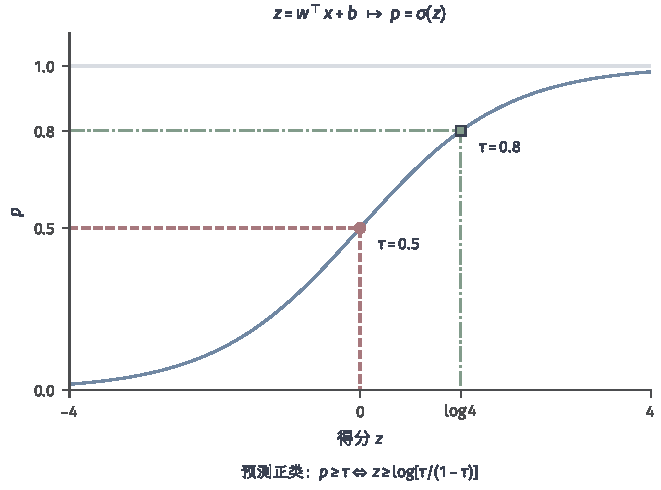
\includegraphics[width=105.412mm]{figures/04-classic-models/00-shared/matplotlib/classification-logistic-probability/figure.pdf}
  \caption{线性得分$z=\bm{w}^{\top}\bm{x}+b$经Logistic函数转为正类概率$p$。蓝色实线为$p=\sigma(z)$；红色虚线与圆点标出$(0,0.5)$，绿色点划线与方点标出$(\log4,0.8)$。两组辅助线分别连接概率阈值与对应的得分阈值，数值是教学构造，不表示训练或校准结果。}
  \label{fig:classification-logistic-probability}
\end{figure}

\subsubsection{参数学习}
\label{sec:classification-logistic-learning}

对独立样本，模型给出的标签概率为$p_i^{y_i}(1-p_i)^{1-y_i}$，其中$p_i=\sigma(\bm{w}^{\top}\bm{x}_i+b)$。\term{最大似然估计}（maximum likelihood estimation, MLE）选择使已观察标签最可能出现的参数。其条件对数似然为
\begin{equation}
  \label{eq:classification-logistic-likelihood}
  \ell(\bm{w},b)
  =\sum_{i=1}^{n}
  \bigl[y_i\log p_i+(1-y_i)\log(1-p_i)\bigr].
\end{equation}
最大化$\ell$等价于最小化负对数似然$L=-\ell$，也就是二分类\term{交叉熵损失}（cross-entropy loss）：给真实标签分配的概率越低，惩罚越大。令增广输入$\tilde{\bm{x}}_i=(\bm{x}_i^{\top},1)^{\top}$、参数$\bm{\beta}=(\bm{w}^{\top},b)^{\top}\in\mathbb{R}^{d+1}$，并记$z_i=\tilde{\bm{x}}_i^{\top}\bm{\beta}$，可写成
\begin{equation}
  \label{eq:classification-logistic-loss}
  L(\bm{\beta})
  =\sum_{i=1}^{n}\bigl[\log(1+e^{z_i})-y_i z_i\bigr].
\end{equation}
数值计算不宜先求极端概率再取对数，可用$\log(1+e^z)=\max\{0,z\}+\log(1+e^{-|z|})$避免指数溢出。

为确定更新方向，利用$\sigma'(z)=\sigma(z)[1-\sigma(z)]$求导。令$\tilde{\bm{X}}\in\mathbb{R}^{n\times(d+1)}$的第$i$行为$\tilde{\bm{x}}_i^{\top}$，$\bm{p}=(p_1,\ldots,p_n)^{\top}$、$\bm{y}=(y_1,\ldots,y_n)^{\top}$，则
\begin{equation}
  \label{eq:classification-logistic-derivatives}
  \begin{aligned}
    \nabla L(\bm{\beta})
      &=\tilde{\bm{X}}^{\top}(\bm{p}-\bm{y}),\\
    \nabla^2 L(\bm{\beta})
      &=\tilde{\bm{X}}^{\top}\bm{R}\tilde{\bm{X}},\\
    \bm{R}
      &=\operatorname{diag}\bigl(p_i(1-p_i)\bigr)_{i=1}^{n}.
  \end{aligned}
\end{equation}
梯度中的$p_i-y_i$是预测概率与观察标签的差。对任意$\bm{v}\in\mathbb{R}^{d+1}$，Hessian的二次型为
\[
  \bm{v}^{\top}\nabla^2L\,\bm{v}
  =\sum_{i=1}^{n}p_i(1-p_i)
    (\tilde{\bm{x}}_i^{\top}\bm{v})^2\geq0.
\]
所以负对数似然$L$是凸函数，而被最大化的$\ell$是凹函数。有限参数处的$p_i(1-p_i)>0$；若$\tilde{\bm{X}}$列满秩，$L$严格凸，否则可能存在不改变训练得分的平坦方向。这涉及\term{可识别性}（identifiability）：数据能否区分不同参数。即使严格凸，也只能保证有限极小点若存在便唯一，不能保证它一定存在。

例如，若存在$\bm{\beta}_0$使$(2y_i-1)\tilde{\bm{x}}_i^{\top}\bm{\beta}_0>0$对所有样本成立，沿$t\bm{\beta}_0$令$t\to\infty$，每项损失均趋于零，但任意有限$t$的损失仍大于零。完全分离的数据因此没有有限MLE；准完全分离也可能使部分参数发散。完整的存在性分析需要区分分离、准分离和重叠情形\scite{albert1984existence}。

实际训练常加入$\lambda\lVert\bm{w}\rVert_2^2/2$，其中$\lambda>0$。这个$L_2$惩罚抑制权重无限增大，也改善病态方向的数值条件。若两类均有样本，所有权重都受惩罚而偏置不受惩罚，所得二分类目标仍有唯一有限极小点；但若训练集只有一类，偏置仍可独自趋于无穷。若连偏置也作正的二次惩罚，则整个增广参数方向都受约束。使用$\lambda\lVert\bm{w}\rVert_1$可得到稀疏权重，但目标不再处处可微，需要适合非光滑目标的求解步骤。

求解器的选择取决于数据规模和存储成本。稠密数据的一轮完整梯度计算为$O(nd)$，构造Hessian约为$O(nd^2)$，直接分解又需要$O(d^3)$。若存储$d\times d$量级的Hessian过于昂贵，\term{有限内存拟牛顿法}（limited-memory BFGS, L-BFGS）只保留少量历史更新来近似二阶信息。大规模稀疏数据则可采用\term{随机梯度下降}（stochastic gradient descent, SGD），每次用一个样本或小批量近似完整梯度。样本数、稀疏程度和精度要求共同决定求解选择。

中小规模问题还可用牛顿法。把正则项加入梯度与Hessian后，每轮解$\bm H_t\bm d_t=-\nabla F(\bm\beta^{(t)})$，再以带阻尼的$\bm\beta^{(t+1)}=\bm\beta^{(t)}+\eta_t\bm d_t$更新；$F$是当前受惩罚目标。第\ref{sec:regression-glm}节已把同一步改写成IRLS：按当前概率产生工作响应和权重，再解加权最小二乘。这里沿用其计算，不把工作响应误当作固定的新标签。实现应解线性方程而不显式求逆，并检查目标变化、梯度与预算；极端概率、病态设计或过大的完整牛顿步都需要数值处理。

\paragraph{多类概率的表示与学习}

\label{sec:classification-logistic-softmax}

从垃圾邮件判断转到新闻主题分类，候选类别可以是体育、科技、文化等多个互斥主题。若分别训练“是否属于某主题”的二分类概率模型，它们的输出未必相加等于$1$；同一篇新闻可能在多个模型中都得到较高概率。我们需要一个共同描述类别竞争的模型。\term{Softmax回归}（softmax regression，也称multinomial logistic regression）为每类建立一个得分，再通过共同分母把这些得分转成和为一的概率向量。其表示约束是任意两类的对数概率比为线性函数。

\textbf{模型结构。}为每类引入$\bm{w}_c\in\mathbb{R}^{d}$和$b_c\in\mathbb{R}$，令$z_c(\bm{x})=\bm{w}_c^{\top}\bm{x}+b_c$。其后验模型为
\begin{equation}
  \label{eq:classification-softmax-model}
  p_c(\bm{x})
  =\mathbb{P}(y=c\mid\bm{x})
  =\frac{\exp z_c(\bm{x})}
         {\sum_{r=1}^{C}\exp z_r(\bm{x})}.
\end{equation}
指数保证概率为正，分母保证归一化；两类之间的分母相消，得到
\[
  \log\frac{p_c(\bm{x})}{p_r(\bm{x})}
  =(\bm{w}_c-\bm{w}_r)^{\top}\bm{x}+b_c-b_r.
\]
当$C=2$时，$p_1(\bm{x})=\sigma((\bm{w}_1-\bm{w}_2)^{\top}\bm{x}+b_1-b_2)$。把第1类视为正类、第2类视为负类，就回到二分类Logistic回归。

共同增加得分不会改变概率。更具体地，对任意$\bm{a}\in\mathbb{R}^{d}$和$t\in\mathbb{R}$，变换$\bm{w}_c\mapsto\bm{w}_c+\bm{a}$、$b_c\mapsto b_c+t$使每个指数项同乘$\exp(\bm{a}^{\top}\bm{x}+t)$，因而全部约掉。这是$d+1$维的参数冗余。选择第$C$类为\term{参考类}（reference class），就是把该类完整的增广参数固定为零：
\begin{equation}
  \label{eq:classification-softmax-reference}
  \begin{gathered}
    \bm{w}_C=\bm{0},\qquad b_C=0,\\
    \log\frac{p_c(\bm{x})}{p_C(\bm{x})}
    =\bm{w}_c^{\top}\bm{x}+b_c
    \quad(c<C).
  \end{gathered}
\end{equation}
参考类约束需同时固定权重与偏置。$\lambda\sum_c\lVert\bm{w}_c\rVert_2^2/2$只消除共同权重平移，还须例如令$\sum_c b_c=0$或惩罚全部偏置，才能锁定共同偏置平移。参数冗余消除后，设计矩阵的秩决定数据能否区分剩余方向，数据分离则影响有限解的存在性。

\textbf{参数学习。}现在$y_i\in\{1,\ldots,C\}$，记$p_{i,c}=p_c(\bm{x}_i)$，$\bm{\Theta}\in\mathbb{R}^{(d+1)\times C}$的第$c$列为$\bm{\beta}_c=(\bm{w}_c^{\top},b_c)^{\top}$。多类负对数似然是
\begin{equation}
  \label{eq:classification-softmax-loss}
  \begin{aligned}
    L(\bm{\Theta})
      &=-\sum_{i=1}^{n}\log p_{i,y_i}\\
      &=\sum_{i=1}^{n}\left[
        \log\sum_{c=1}^{C}e^{z_c(\bm{x}_i)}
        -z_{y_i}(\bm{x}_i)\right].
  \end{aligned}
\end{equation}
多分类同样可以通过迭代优化学习参数。为构造每轮更新，先对上述损失求导；以$\mathbb{1}\{\cdot\}$表示条件成立时为一、否则为零的指示函数，得到
\begin{equation}
  \label{eq:classification-softmax-gradient}
  \begin{aligned}
    \nabla_{\bm{w}_c}L
      &=\sum_{i=1}^{n}
        [p_{i,c}-\mathbb{1}\{y_i=c\}]\bm{x}_i,\\
    \frac{\partial L}{\partial b_c}
      &=\sum_{i=1}^{n}
        [p_{i,c}-\mathbb{1}\{y_i=c\}].
  \end{aligned}
\end{equation}
梯度仍由“预测概率减观察标签”组成。目标凸，但共同参数平移及秩亏可能带来平坦方向，分离数据也可能没有有限MLE。参考类约束消除表示冗余，正则化控制参数大小，两者的作用不同。

Softmax可用分块牛顿法、L-BFGS或小批量SGD优化，多类Hessian还包含类别间的耦合，不能简单把$C$个独立的二分类IRLS问题拼起来。求概率时应先减去$m(\bm{x})=\max_c z_c(\bm{x})$，用$e^{z_c-m}/\sum_r e^{z_r-m}$得到完全相同且更稳定的结果。普通稠密实现的一轮梯度计算约为$O(ndC)$。

预测可取$\hat y(\bm{x})=\argmax_c p_c(\bm{x})=\argmax_c z_c(\bm{x})$，并按固定类别次序处理平局。共同分母不改变得分排序，所以只需输出一个类别时，可以直接比较各类得分。

\paragraph{交叉熵在拟合什么}
\label{sec:classification-logistic-theory}
记真实类别后验为$\bm\eta(\bm x)$，预测概率向量为$\bm p(\bm x)$。固定输入时，预测交叉熵减去真实后验的熵为
\[
 -\sum_c\eta_c\log p_c+\sum_c\eta_c\log\eta_c
 =D_{\mathrm{KL}}(\bm\eta\Vert\bm p)\geq0.
\]
因此最理想的条件概率目标是真实后验；使用有限参数的Logistic或Softmax时，只能在所设定的对数几率关系中拟合它。若目标的对数几率需要平方或交互项，应改变输入特征，而不是只增加优化轮数。分类又只取最大概率的类别，所以概率拟合误差与分类错误是不同的评价对象。

\subsubsection{概率校准与温度缩放}

\label{sec:classification-probability-calibration}

需要用概率设定邮件拦截门槛时，还要检查报告的置信度能否对应实际频率。Softmax输出满足概率公理，却不自动满足\term{概率校准}（probability calibration）。例如，在报告某类概率约为$0.8$的一组样本中，该类的实际比例也应接近$0.8$。有限样本、模型失配、正则化和分布变化都可能破坏这种对应。这里检验的是报告概率与实际频率的联系，和按最大概率选择类别是不同的问题。

一种简洁的后处理是温度缩放（temperature scaling）：固定已训练得分$z_c(\bm x)$，只学习$T>0$，令$\tilde p_c(\bm x)=\exp(z_c/T)/\sum_r\exp(z_r/T)$。用未参与原模型拟合的校准记录最小化这组概率的负对数似然，就可估计温度；随后还要在另一份独立数据上评价。正温度不改变最高得分类别，却会改变概率的集中程度。Guo等在其研究的网络和数据上比较了这类方法；单一温度不能保证修复所有概率失配\scite{guo2017calibration}。

\subsubsection{层次Softmax、NCE与负采样}

\paragraph{降低大类别集的概率计算成本}
\label{sec:classification-softmax-hierarchical}

类别特别多时，平坦Softmax要在分母中累加全部类别的指数得分。\term{层次Softmax}（hierarchical softmax）改用树上路径概率的乘积表示一个类别的概率，把一次类别选择拆成沿路径进行的条件选择。这改变了概率的参数化方式，计算某个类别概率时可以沿相应路径展开；类别怎样组织成树，也就成为模型设计的一部分。若需要全部类别概率，计算负担仍然存在，沿路径计算一个类别的概率也不等于已经找到了最高概率类别\scite{goodfellow2016}。

用四个类别构造一个二叉树例子，可以分别看清归一化和搜索。把类别1、2放在根的左子树，类别3、4放在右子树。固定当前输入，设根节点向左的条件概率为$0.6$、向右为$0.4$；到达左子树以后，两片叶的条件概率为$0.5,0.5$；到达右子树以后，两片叶的条件概率为$0.99,0.01$。于是
\[
  \begin{aligned}
    p_1&=0.6\times0.5=0.3,&
    p_2&=0.6\times0.5=0.3,\\
    p_3&=0.4\times0.99=0.396,&
    p_4&=0.4\times0.01=0.004.
  \end{aligned}
\]
四类概率相加为一，因为每个内部节点都把到达它的概率质量完整分给两个孩子。内部节点可以各用一个Logistic模型给出两条分支的条件概率；一旦指定叶子，只需计算沿途节点，不必访问无关分支。在平衡二叉树中，路径长度约为$\log_2C$，不平衡树的路径则可能更长。给定类别树后，一条训练记录的真实类别就确定沿途的二元分支标签；训练时把这些节点的Logistic对数概率相加，沿路径求梯度并更新节点参数，无须访问无关分支。树的安排固定了哪些类别共享前面的判断，需要作为模型结构选择。

这个例子还表明，根处贪心选择较大的左支会错过概率最大的第3类。因此，计算指定类别的概率、找最高概率类别与输出全部类别概率，是三种不同的计算任务。

\paragraph{减少显式归一化的训练负担}
\label{sec:classification-softmax-noise-contrast}

当归一化分母需要对大量候选求和时，也可以改变概率估计所用的训练问题。\term{噪声对比估计}（noise-contrastive estimation, NCE）通过区分数据与人为噪声来估计模型，训练时回答一条记录来自数据还是人为噪声，模型参数也决定这项区分的得分。归一化常数可以与模型参数一起估计，避免每一步都对全部候选得分显式求和。它与层次Softmax改变的位置不同：前者改变估计问题，后者把类别概率分解到树上，不能把两者都当作原平坦Softmax公式的计算改写\scite{goodfellow2016}。

沿用新闻主题分类，可以把这一辅助任务写出来。固定输入$\bm x$，原任务的随机变量$Y$仍表示新闻主题，真实后验为$\eta_c(\bm x)$。现在对每一条真实记录$(\bm x,c^+)$，从已知、可抽样且可求值的噪声分布$q(c\mid\bm x)$独立抽取$k\geq1$个类别，组成噪声配对；这里取$q(c\mid\bm x)>0$覆盖全部候选类别。另引入二元来源标签$D$：真实配对的$D=1$，人为噪声配对的$D=0$。$D$回答配对怎样产生，$Y$回答新闻属于哪个主题，两者不是同一个类别变量。噪声抽样也可能恰好得到$c^+$，这不改变它的来源标签；若排除这种抽样结果，就必须相应改变噪声分布。

一条真实记录配$k$条噪声，意味着在混合记录中，两个来源的比例为$1:k$，而不是各占一半。固定同一个$\bm x$后，由贝叶斯公式，真实的来源后验为
\[
  \mathbb P(D=1\mid\bm x,c)
  =\frac{\eta_c(\bm x)}
    {\eta_c(\bm x)+kq(c\mid\bm x)}.
\]
这个式子把原主题后验接到了新增的来源区分任务上。NCE用原模型的非负质量替换未知的$\eta_c$。具体地，保留类别得分$z_{\theta,c}(\bm x)$，另外用可计算函数$\kappa_{\psi}(\bm x)$估计其对数归一化量，定义
\begin{equation}
  \label{eq:classification-nce-source-model}
  \begin{aligned}
    a_{\theta,\psi}(c\mid\bm x)
      &=\exp\{z_{\theta,c}(\bm x)-\kappa_{\psi}(\bm x)\},\\
    h_{\theta,\psi}(\bm x,c)
      &=\frac{a_{\theta,\psi}(c\mid\bm x)}
        {a_{\theta,\psi}(c\mid\bm x)+kq(c\mid\bm x)}\\
      &=\sigma\bigl(z_{\theta,c}(\bm x)-\kappa_{\psi}(\bm x)
                  -\log[kq(c\mid\bm x)]\bigr).
  \end{aligned}
\end{equation}
$\theta$控制原类别得分，$\psi$控制归一化量的函数表示；二者通过$h$共同影响来源预测。训练中$\kappa_{\psi}(\bm x)$不必已经等于$\log\sum_r e^{z_{\theta,r}(\bm x)}$，所以$a_{\theta,\psi}$暂时未必在类别上相加为一；但$h$始终是严格介于零和一之间的二元预测。条件模型的归一化量一般随$\bm x$变化，不能未经假设就用一个共享常数代替。所选$\kappa_{\psi}$的表示与求值也有成本，需要另行规定；若它不能表示所需的归一化函数，估计便会受到这项限制。

令第$i$条真实记录为$(\bm x_i,y_i)$，对应噪声类别为$c^-_{i,1},\ldots,c^-_{i,k}$。既然要提高真实配对来自数据的预测概率，同时提高噪声配对来自噪声的预测概率，每条记录的辅助对数目标就是
\begin{equation}
  \label{eq:classification-nce-objective}
  \begin{aligned}
    J_i^{\mathrm{NCE}}(\theta,\psi)
      &=\log h_{\theta,\psi}(\bm x_i,y_i)\\
      &\quad+\sum_{j=1}^{k}
        \log[1-h_{\theta,\psi}(\bm x_i,c^-_{i,j})].
  \end{aligned}
\end{equation}
对训练记录求和并最大化这个目标，就把原模型参数与归一化参数接入同一项来源分类训练。每次计算只访问真实类别和抽中的$k$个类别得分，无需在该步显式计算全类别指数和；噪声抽样、噪声概率与$\kappa_{\psi}$的计算成本仍需计入。

来源概率与主题概率的数值也不同。例如，三个主题使用均匀噪声，取$k=2$；若某主题的真实后验为$0.6$，则相应来源后验为$0.6/(0.6+2/3)\approx0.474$。因此不能把训练得到的$h$直接当作原主题后验。NCE的统计结论还依赖噪声支持、模型正确指定、归一化函数的可表示性、可识别性以及抽样和优化条件；上述构造没有证明有限样本下$a$已经精确归一化，也没有把辅助目标与原Softmax似然说成同一个目标。若预测接口要求完整的主题概率向量，仍需明确恢复或计算类别归一化，并另外检查校准。

\paragraph{减少每步训练的负例比较}
\label{sec:classification-softmax-negative-sampling}

若每次更新都比较全部其他类别，训练计算会随类别集增大。\term{负采样}（negative sampling）只对抽取的负例建立局部区分目标，减少这一步参与比较的对象。它通常改变原Softmax训练目标，因而应按实际采用的目标解释训练结果；需要类别概率时，也不能直接把局部区分得分当成前面归一化的概率向量\scite{goodfellow2016}。

继续使用一条真实配对与$k$条噪声配对，令$s_\theta(\bm x,c)$为可训练的配对得分。一种常见负采样目标为
\begin{equation}
  \label{eq:classification-negative-sampling-objective}
  \begin{aligned}
    J_i^{\mathrm{NEG}}(\theta)
      &=\log\sigma(s_\theta(\bm x_i,y_i))\\
      &\quad+\sum_{j=1}^{k}
        \log\sigma(-s_\theta(\bm x_i,c^-_{i,j})).
  \end{aligned}
\end{equation}
第一项提高真实配对的得分，第二项降低噪声配对的得分。两种方法都用少量配对训练二元区分，但上面的NCE把区分得分明确写成原模型对数质量减去$\log[kq(c\mid\bm x)]$；这个负采样目标的样本项只使用$s_\theta$，没有显式使用该噪声概率修正和归一化函数。噪声分布仍通过抽样影响训练结果，不能理解成负采样与$q$无关。若没有另外建立从$s_\theta$恢复类别概率的关系，$\sigma(s_\theta)$表示的仍是辅助区分预测，不是各主题相加为一的后验；也不能把该目标解释成仅从原Softmax分母删除未抽中的项。

\subsubsection{稀疏概率核模型：相关向量机}
\label{sec:classification-rvm}

核SVM用支持向量形成得分；若希望同时学习概率，并压缩预测时需要的基函数，可以采用Tipping的\term{相关向量机}（relevance vector machine, RVM）。它沿用Logistic概率，却把得分写成$g(\bm x)=\sum_{j=1}^m w_j\phi_j(\bm x)$；候选基函数通常取训练点为中心的核函数并加入常数项。每个系数分别有先验$w_j\sim\mathcal N(0,\alpha_j^{-1})$，其中$\alpha_j>0$是待学精度，即方差的倒数。精度大时，该基函数的系数受到更强收缩，而不是预先规定哪些样本必须成为支持向量\scite{tipping2001rvm}。

固定精度后，先以原伯努利似然乘这些高斯先验，最大化后验；这等价于最小化Logistic负对数似然加$\bm w^\top\bm A\bm w/2$，其中$\bm A=\operatorname{diag}(\alpha_1,\ldots,\alpha_m)$。牛顿或IRLS求得众数$\hat{\bm w}$后，RVM用众数附近的高斯近似来描述后验，这称为Laplace近似。令$\bm\Phi\in\mathbb R^{n\times m}$满足$\bm\Phi_{i,j}=\phi_j(\bm x_i)$，以$p_i=\sigma(g(\bm x_i))$记当前正类概率，并令$\bm B=\operatorname{diag}(p_i(1-p_i))_{i=1}^n$，则$m\times m$的近似协方差为
\[
  \bm\Sigma=(\bm\Phi^\top\bm B\bm\Phi+\bm A)^{-1}.
\]
原方法再依据近似边缘似然更新精度，例如使用固定点更新$\alpha_j\leftarrow(1-\alpha_j\bm\Sigma_{j,j})/\hat w_j^2$，并交替重算后验众数与协方差。数值上按阈值剔除受到强收缩的基函数，配合目标变化或迭代预算停止；分母过小等退化情况需要数值处理，精度学习也不保证全局最优。

最终保留的基函数及其系数构成稀疏预测器。若对近似后验积分，得到的是近似贝叶斯类别概率；只代入众数则是点估计预测，二者应区分。RVM改变了SVM的间隔准则和参数选择机制，有限精度只保证收缩，不保证系数恰为零；稀疏程度、计算收益与概率质量仍需验证。

\subsection{朴素贝叶斯}
\label{sec:classification-naive-bayes}

判断一封邮件是不是垃圾邮件，也可以换个问法：“如果它是垃圾邮件，有多大概率出现这些词？如果是正常邮件呢？”比较这两个问题的答案，再结合两类邮件各自的比例，就能反推它属于垃圾邮件的概率。如果以$d$个词是否出现作为二值特征，完整类条件分布就有$2^d$种输入组合；即使只选20个词，也已有一百多万种组合，很多组合在训练集中一次都没有出现。逐项估计它们的概率，需要远多于单个词频统计的数据，其中绝大部分组合的计数都会是零。

要打破这个组合爆炸，可以作一个简化假设：一旦知道了邮件类别，各个词是否出现就彼此无关。这并不要求现实中词与词真的独立——给定“这是垃圾邮件”之后，“免费”和“领取”仍可能一起出现——而是用一个乘积近似来换取可计算性。\term{朴素贝叶斯}（naive Bayes, NB）正是基于给定类别后各特征条件独立这一假设，把单个特征的概率相乘，得到输入的类条件概率。这样，无需等待整套词语组合反复出现，就能从各词的计数估计类别证据。简化也会遗漏词语依赖：例如给定邮件类别后，“免费”与“领取”仍可能共同出现得更多。模型用较少统计量换取可直接计算的估计，样本波动可能减小，依赖假设造成的偏差则仍会保留。

Maron在1961年关于自动索引的研究，是概率方法用于文档归类的早期工作之一。文档分类需要从大量词项中提取可累积的类别证据，这也成为朴素贝叶斯的一项典型用途\scite{maron1961indexing}。

\subsubsection{模型结构}
\label{sec:classification-naive-bayes-structure}

对一般特征向量，NB采用给定类别后的\term{条件独立}（conditional independence）假设：已知$y=c$后，一个特征的取值不再改变其他特征的分布。令$\pi_c=\mathbb{P}(y=c)$、$p_{j,c}(x_j)=p(x_j\mid y=c)$，模型写成
\begin{equation}
  \label{eq:classification-naive-bayes-model}
  \begin{aligned}
    q_c(\bm{x})&=\prod_{j=1}^{d}p_{j,c}(x_j),\\
    \mathbb{P}_{\mathrm{NB}}(y=c\mid\bm{x})
      &=\frac{\pi_c q_c(\bm{x})}
      {\sum_{r=1}^{C}\pi_r q_r(\bm{x})}.
  \end{aligned}
\end{equation}
记号$q_c$强调这是模型使用的乘积分布，未必等于真实类条件分布。条件独立不要求全部训练样本混在一起时特征仍独立，例如词项之间的总体相关性可能部分来自主题差异。

只需要分类时，各类共同的分母可以省略。为避免许多小概率连乘下溢，通常比较对数得分
\begin{equation}
  \label{eq:classification-naive-bayes-score}
  s_c(\bm{x})
  =\log\pi_c+\sum_{j=1}^{d}\log p_{j,c}(x_j),
  \qquad
  \hat y(\bm{x})=\argmax_c s_c(\bm{x}).
\end{equation}
这里$s_c$不是归一化的对数后验；需要概率时还须减去$\log\sum_r e^{s_r}$。零概率可使得分为负无穷，后面的平滑正是为未见事件保留概率质量。文档的多项式版本沿用相似得分，但它的独立性对象是词元位置，而非总长度固定后的各维计数，必须另外说明。

\subsubsection{参数学习}
\label{sec:classification-naive-bayes-learning}

令$n_c=\sum_i\mathbb{1}\{y_i=c\}$，类先验的MLE为$\hat\pi_c=n_c/n$。这是以训练样本的类别比例估计目标总体的比例，依赖抽样具有代表性；人为重采样改变类别比例，部署先验需要按抽样机制修正或另行估计。也可以使用有依据的外部类别比例；若希望保留对该比例的不确定性，并为训练中未见的类别保留概率质量，则可对类概率向量$\bm{\pi}=(\pi_1,\ldots,\pi_C)^{\top}$设置参数先验。以下对类别概率与各组类条件参数设置相互独立的先验，以便分别更新。

若使用正参数$\gamma_c$的Dirichlet参数先验，观察类别计数后的参数变为$\gamma_c+n_c$，相应后验均值为
\[
  \tilde\pi_c=\frac{n_c+\gamma_c}{n+\sum_r\gamma_r}.
\]
伪计数使未见类别仍有正概率；其总量控制先验相对于数据的影响。“类别先验$\pi_c$”属于样本生成模型，“对$\bm\pi$设置参数先验”描述估计它之前的不确定性，两者不能混同。Dirichlet分布的形式可参考\BookChapterRef{chap:random-variables}{卷二《数学准备：概率、因果与决策》的“随机变量”章}。

连续特征可采用\term{高斯朴素贝叶斯}（Gaussian naive Bayes），即$x_j\mid y=c\sim\mathcal{N}(\mu_{j,c},\sigma_{j,c}^{2})$，其中$\sigma_{j,c}^{2}>0$。当$n_c>0$且该特征的类内平方偏差和为正时，均值和方差的MLE为
\begin{equation}
  \label{eq:classification-naive-bayes-gaussian}
  \begin{aligned}
    \hat\mu_{j,c}
      &=\frac{1}{n_c}\sum_{i:y_i=c}x_{i,j},\\
    \hat\sigma_{j,c}^{2}
      &=\frac{1}{n_c}\sum_{i:y_i=c}
        (x_{i,j}-\hat\mu_{j,c})^2.
  \end{aligned}
\end{equation}
方差分母为$n_c$，不是无偏样本方差所用的$n_c-1$。在上述条件下，预测时将这些量代入一维高斯密度后相乘。若某类某特征恒定为$a$，固定$\mu_{j,c}=a$后，对数似然为$-n_c\log(2\pi\sigma_{j,c}^{2})/2$，随正方差趋于零而无界增大。因此，此时正方差参数域内没有有限MLE；式\eqref{eq:classification-naive-bayes-gaussian}给出的零值只是样本散度，不能代入普通高斯密度。设定有明确尺度的方差下限或加入先验后，得到的是相应的受约束或正则化估计；给密度任意“加一”不是离散概率的平滑对应物。

只关心某个词是否出现时，可用\term{伯努利朴素贝叶斯}（Bernoulli naive Bayes）。输入$x_{i,j}\in\{0,1\}$，令$n_{j,c}=\sum_{i:y_i=c}x_{i,j}$，则
\begin{equation}
  \label{eq:classification-naive-bayes-bernoulli}
  \begin{aligned}
    q_c(\bm{x})
      &=\prod_{j=1}^{d}
        \theta_{j,c}^{x_j}(1-\theta_{j,c})^{1-x_j},\\
    \hat\theta_{j,c}&=\frac{n_{j,c}}{n_c}.
  \end{aligned}
\end{equation}
$x_j=0$也通过词缺失概率提供证据，因此两种取值的项都参与得分；这里的MLE要求$n_c>0$。
为平滑这个二值事件，使用Beta分布作为$\theta_{j,c}$的先验，
两个正参数$\alpha_1,\alpha_0$分别对应出现与未出现。乘以似然后，
两项指数分别增加$n_{j,c}$和$n_c-n_{j,c}$，所以
\[
  \theta_{j,c}\mid D_n
  \sim\operatorname{Beta}
    (\alpha_1+n_{j,c},\,\alpha_0+n_c-n_{j,c}).
\]
其后验均值为$(n_{j,c}+\alpha_1)/(n_c+\alpha_1+\alpha_0)$；对称情形$\alpha_1=\alpha_0=\alpha$的分母是$n_c+2\alpha$。这同时平滑了出现和未出现两种事件。

若重复出现的次数也有意义，应使用\term{多项式朴素贝叶斯}（multinomial naive Bayes）。设固定词表有$d$个词项，$\bm{x}_i\in\mathbb{N}_0^d$记录一篇文档的词项计数，$m_i=\sum_jx_{i,j}$是该文档的总词元数。给定类别和$m_i$，假设每个词元位置独立地按$\bm{\theta}_c=(\theta_{1,c},\ldots,\theta_{d,c})^{\top}$抽取词项，其中$\sum_j\theta_{j,c}=1$。忽略顺序后，计数向量服从
\begin{equation}
  \label{eq:classification-naive-bayes-multinomial}
  \mathbb{P}(\bm{x}_i\mid y_i=c,m_i)
  =\frac{m_i!}{\prod_{j=1}^{d}x_{i,j}!}
    \prod_{j=1}^{d}\theta_{j,c}^{x_{i,j}}.
\end{equation}
因为计数总和已固定，各维计数并不独立。将它写成每维整数取值的独立类别分布，会改变模型和分母。McCallum与Nigam专门比较了伯努利和多项式这两种文档事件模型，明确区分“词是否出现”与“词出现多少次”\scite{mccallum1998event}。

标准文档分类通常进一步假设长度分布与类别无关，因而$\mathbb{P}(m_i\mid y_i=c)$在类别比较中约掉，此时给定长度后的类先验仍为$\pi_c$。若长度本身携带类别信息，则应保留并估计该项，使长度也参与后验计算。

令$t_{j,c}=\sum_{i:y_i=c}x_{i,j}$为第$c$类中词项$j$的总出现次数，$t_c=\sum_jt_{j,c}$为该类的总词元数。去掉与参数无关的组合系数后，类内对数似然为$\sum_jt_{j,c}\log\theta_{j,c}$。当$t_c>0$时，在$\sum_j\theta_{j,c}=1$约束下求极值，正计数坐标上的拉格朗日方程给出$t_{j,c}/\theta_{j,c}$为同一常数，零计数坐标取零；求和确定常数为$t_c$，从而得到频率MLE。

若对$\bm{\theta}_c$使用$\operatorname{Dirichlet}(\alpha_1,\ldots,\alpha_d)$先验，其中$\alpha_j>0$，同样的共轭更新把各坐标的幂次从$\alpha_j-1$变为$\alpha_j+t_{j,c}-1$，得到
\[
  \bm{\theta}_c\mid D_n
  \sim\operatorname{Dirichlet}
    (\alpha_1+t_{1,c},\ldots,\alpha_d+t_{d,c}).
\]
把更新后的参数归一化即可得到后验均值。两种估计分别为
\begin{equation}
  \label{eq:classification-naive-bayes-smoothing}
  \hat\theta_{j,c}=\frac{t_{j,c}}{t_c},
  \qquad
  \tilde\theta_{j,c}
  =\frac{t_{j,c}+\alpha_j}
         {t_c+\sum_{r=1}^{d}\alpha_r}.
\end{equation}
前式要求$t_c>0$；后式也给出下一词元的后验预测概率，因为给定参数时该概率为$\theta_{j,c}$，对参数后验积分便得到其后验均值。这种均值估计通常既不同于MLE，也不同于式\eqref{eq:regression-map}定义的MAP。对称$\alpha_j=1$给出\term{拉普拉斯平滑}（Laplace smoothing），相当于每个词项加入一个伪计数；$\alpha_j=1/2$对应多项式参数的Jeffreys先验。对伯努利参数，其对应物是$\operatorname{Beta}(1/2,1/2)$，不应把这些常数不加区分地推广到高斯方差。以平滑估计代入式\eqref{eq:classification-naive-bayes-multinomial}得到的是常用的点估计分类器，不等于积分消去参数后的整篇文档预测分布。

在长度与类别无关的约定下，文档预测只需计算$\log\tilde\pi_c+\sum_jx_j\log\tilde\theta_{j,c}$。算法\ref{alg:classification-multinomial-nb}给出完整的统计与预测流程，训练和预测使用相同的词表，并明确处理平滑与得分平局。
\begin{algorithm}[带平滑的多项式朴素贝叶斯]
  \label{alg:classification-multinomial-nb}
  \begin{algorithmic}[1]
    \Require 非空训练集$D_n$，固定词表大小$d$与类别数$C$；
    \Statex \hspace{\algorithmicindent} 词项伪计数$\alpha>0$，类别伪计数$\gamma>0$
    \Ensure 类先验$\tilde{\bm{\pi}}$、词项概率$\tilde{\bm{\Theta}}$及预测规则
    \State 检查所有输入为有限非负整数计数，标签属于$\{1,\ldots,C\}$
    \State 将$n_c$、$t_c$与$t_{j,c}$全部初始化为零
    \For{$i=1,\ldots,n$}
      \State 令$c=y_i$，并更新$n_c\gets n_c+1$
      \For{满足$x_{i,j}>0$的词项$j$}
        \State $t_{j,c}\gets t_{j,c}+x_{i,j}$
        \State $t_c\gets t_c+x_{i,j}$
      \EndFor
    \EndFor
    \For{$c=1,\ldots,C$}
      \State $\tilde\pi_c\gets(n_c+\gamma)/(n+C\gamma)$
      \State 对所有$j$，令$\tilde\theta_{j,c}\gets(t_{j,c}+\alpha)/(t_c+d\alpha)$
    \EndFor
    \State 对新计数向量$\bm{x}$，按相同词表与输入检查计算
    \Statex \hspace{\algorithmicindent}
      $s_c=\log\tilde\pi_c+\sum_{j:x_j>0}x_j\log\tilde\theta_{j,c}$
    \State 返回$s_c$最大的类别；平局时返回索引最小的类别
  \end{algorithmic}
\end{algorithm}

假设词表只有三个词项，两类累计计数分别为$(3,1,0)$和$(0,1,3)$，类先验均为$1/2$。取$\alpha=1$，平滑后的词项概率分别为$(4,2,1)/7$和$(1,2,4)/7$。对新文档$\bm{x}=(1,0,1)^{\top}$，两类乘积相同，判决平局；对$\bm{x}=(2,0,1)^{\top}$，两类得分之差为$\log4$，于是选择第1类。这个教学例子显示了重复计数怎样改变证据，而零计数词项经平滑后不会把整类概率直接清零。

\paragraph{依赖为何可能改变概率却不改变类别}
\label{sec:classification-naive-bayes-theory}
模型失配时，更多计数可以使乘积分布的估计稳定，却不能恢复被独立假设省掉的关系。例如，把一个有信息的二值特征复制一次，在等类先验下，NB会把原似然比平方：真实比值为4时后验为$4/5$，重复计算后却报$16/17$。最高类别没有改变，置信度已经失真；先验不等时，重复证据还可能改变类别。分类排序与概率质量因而需要分别检查，不能只因存在相关性就断言分类必然失败，也不能因分类正确就接受输出概率\scite{domingos1997optimality}。

\subsubsection{AODE：保留部分特征依赖}

\label{sec:classification-naive-bayes-dependence-extension}

朴素贝叶斯按单个特征累计证据，类内条件独立假设会省略特征之间的联系。若同一类别中的“免费”与“领取”经常共同出现，单独累计两个词的频数仍会遗漏这段关系。\term{平均单依赖估计器}（averaged one-dependence estimators, AODE）让每个依赖模型以一个特征作为共同父特征，再平均这些模型的联合得分。各个模型假设其余特征在同时给定类别和父特征后条件独立，从而保留部分成对关系。Webb、Boughton与Wang在2005年研究了这一方法；代价是更多条件计数、存储与预测计算，条件样本不足时也可能难以估计这些额外关系\scite{webb2005aode}。

把“免费”“领取”“优惠”是否出现记为三个二值特征，就能写出父特征实际改变了哪个条件。回到$C$个类别，固定当前输入$\bm x=(x_1,x_2,x_3)^\top$，以下用$p(c,x_j)$简写类别与父特征取值的联合概率，用$p(x_l\mid c,x_j)$简写同时给定这两者后的条件概率。三个单依赖模型的当前联合得分分别为
\[
  \begin{aligned}
    q_{1,c}(\bm x)
      &=p(c,x_1)p(x_2\mid c,x_1)p(x_3\mid c,x_1),\\
    q_{2,c}(\bm x)
      &=p(c,x_2)p(x_1\mid c,x_2)p(x_3\mid c,x_2),\\
    q_{3,c}(\bm x)
      &=p(c,x_3)p(x_1\mid c,x_3)p(x_2\mid c,x_3).
  \end{aligned}
\]
例如，第一个模型中“领取”的概率既随类别改变，也随“免费”是否出现而改变，这就是把第一个特征称为父特征的含义；其余两个子特征则仍假设在这些条件下独立。与NB相比，变化落在条件计数中，并不要求三个词无条件地互相独立。

并非每个父特征取值都有足够记录支持。令$N_j(x_j)$为训练集中第$j$个特征取当前值$x_j$的记录数，在训练或验证方案中预定最低频数$m\geq1$，并记
\[
  J(\bm x)=\{j\in\{1,2,3\}:N_j(x_j)\geq m\}.
\]
这个集合只选择当前有足够频数的父特征；联合与条件概率仍用相应计数作平滑估计，正平滑使未见的类内组合也有定义。$J(\bm x)$非空时，先平均这些模型的联合得分，再在类别之间归一化：
\begin{equation}
  \label{eq:classification-aode-joint-average}
  \begin{aligned}
    Q_c(\bm x)
      &=\frac{1}{|J(\bm x)|}
          \sum_{j\in J(\bm x)}q_{j,c}(\bm x),\\
    \hat p_c(\bm x)
      &=\frac{Q_c(\bm x)}{\sum_{r=1}^{C}Q_r(\bm x)}.
  \end{aligned}
\end{equation}
只需类别时，可以直接比较$Q_c$并沿用固定的平局规则。这里平均的是联合得分，先把每个模型分别归一化再平均后验，一般会改变各模型的相对权重。若$J(\bm x)$为空，就明确回退到使用同一二值事件模型和平滑方式的NB；不能对空集合取平均。频数门槛与平滑分别处理统计支持和未见组合，仍不能保证增加依赖后一定改善独立数据上的分类或校准。

\subsubsection{补集朴素贝叶斯（CNB）}

\label{sec:classification-naive-bayes-complement}

对文本数据，参数估计还受到类别样本数的影响。一个主题若只有少量文档，某个词的类内计数就可能被个别记录明显改变；其他主题的文档总量却可能充足。\term{补集朴素贝叶斯}（complement naive Bayes, CNB）改用不属于第$c$类的文档构造补集统计，再寻找与该补集不匹配的输入。它改变的是估计词项权重的样本来源，目标仍是预测原来的类别。Rennie等在2003年提出这一方法，针对类别不平衡时的权重估计偏差，并结合其他修正研究文本分类效果\scite{rennie2003complement}。

沿用多项式计数，令$t_{j,\bar c}=\sum_{i:y_i\neq c}x_{i,j}$、$t_{\bar c}=\sum_jt_{j,\bar c}$。先定义补集词项参数及其对数权重：
\begin{equation}
  \label{eq:classification-complement-nb}
  \begin{aligned}
    \tilde\theta_{j,\bar c}
      &=\frac{t_{j,\bar c}+\alpha_j}
              {t_{\bar c}+\sum_{r=1}^{d}\alpha_r},\\
    w_{j,c}&=\log\tilde\theta_{j,\bar c},\\
    s_c^{\mathrm{CNB}}(\bm{x})
      &=\log\pi_c-\sum_{j=1}^{d}x_jw_{j,c}.
  \end{aligned}
\end{equation}
Rennie等给出的CNB规则选择最大$s_c^{\mathrm{CNB}}$；他们同时说明实验中为简化采用均匀类别先验，此时等价于选择补集对数得分$\sum_jx_jw_{j,c}$最小的类别。负号使“不像补集”转化为支持第$c$类的证据：$\tilde\theta_{j,\bar c}$表示补集的词项参数，与正类$\mathbb{P}(\bm{x}\mid y=c)$中的参数是不同对象。补集可能混合多个类别，本身也未必是单一多项式分布，因此CNB按补集统计构造分类得分，正类后验需要另外的概率模型。

补集计数可用全局计数减去类内计数获得。权重归一化、文档长度变换和类别先验处理还会改变最终得分，比较实现时应固定这些设置。补集统计有更多记录可用，也可能混合差异明显的其他主题；分类收益与输出概率仍需在独立数据上检查。

\subsection{高斯判别分析（GDA）}
\label{sec:classification-gda}

高斯NB只保存每维的均值与方差，相当于把类内协方差矩阵的非对角元素设为零。这个约束可能丢失决定类别的信息。设两类二维高斯数据的均值都为零，每一维的方差都为$1$，但类1中两个测量值通常一起增减，类2中则通常一个增大、另一个减小。两类的单维分布完全相同，高斯NB只能依据先验比例判类；联合分布却分别沿两个不同方向伸展。

\term{高斯判别分析}（Gaussian discriminant analysis, GDA）为每类估计多元高斯分布，用协方差保留这种共同变化。在上述例子中，两类不同的非对角协方差进入判别得分，就能利用单维统计量遗漏的方向信息。共享协方差形式对应LDA，各类分别估计协方差则对应QDA。完整协方差同时增加了参数量；样本较少时，收缩估计仍可能比完全放开的估计更合适。

第\ref{sec:clustering-gmm}节的高斯混合模型同样估计高斯成分及其权重，但成分归属是潜变量，通常用\term{期望最大化}（expectation-maximization, EM）交替计算成分归属的后验概率并更新分布参数；两步计算的分类实例见第\ref{sec:classification-self-training-soft-em}节。GDA中的类别标签已经观测，可以直接按类分组估计。两者共享高斯密度结构，却分别服务于预设类别预测和无标签分组。

\subsubsection{模型结构}
\label{sec:classification-gda-structure}

本节用GDA统称各类具有高斯条件分布的判别模型，并分别讨论共享协方差与类特有协方差。对第$c$类，参数是$\pi_c$、$\bm{\mu}_c\in\mathbb{R}^{d}$及对称正定的$\bm{\Sigma}_c\in\mathbb{R}^{d\times d}$：
\begin{equation}
  \label{eq:classification-gda-density}
  \begin{aligned}
    p(\bm{x}\mid y=c)
      &=\frac{\exp[-\Delta_c(\bm{x})/2]}
        {(2\pi)^{d/2}|\bm{\Sigma}_c|^{1/2}},\\
    \Delta_c(\bm{x})
      &=(\bm{x}-\bm{\mu}_c)^{\top}
        \bm{\Sigma}_c^{-1}(\bm{x}-\bm{\mu}_c).
  \end{aligned}
\end{equation}
这里的二次型$\Delta_c$按类内变化尺度衡量输入偏离均值的程度；行列式项补偿分布体积，在不同协方差的类别比较中同样参与得分。贝叶斯后验仍为$\pi_cp(\bm{x}\mid y=c)/\sum_r\pi_rp(\bm{x}\mid y=r)$。

分类采用第\ref{sec:classification-lda-covariance-extensions}节的QDA得分，见式\eqref{eq:classification-qda-score}；这里将其中的估计量换为当前模型的$\pi_c,\bm\mu_c,\bm\Sigma_c$，把所得对数得分记为$g_c(\bm{x})$。预测选择最大$g_c$。这一模型不要求各特征独立，但要求整类分布可由单个多元高斯刻画；完整协方差保留全部二阶关系，单个高斯成分仍限制了非线性依赖和多峰结构的表达。

\subsubsection{参数学习}
\label{sec:classification-gda-learning}

有标签时，各类样本的归属已知，可以直接按类累计统计量。先验与均值按式\eqref{eq:classification-lda-mean-prior}估计；类特有协方差使用第\ref{sec:classification-lda-covariance-extensions}节QDA的类内平方偏差平均，再代入式\eqref{eq:classification-qda-score}判类。要求共享协方差时，则合并各类散度并除以总样本量$n$，回到LDA。两条路线都最大化带标签的联合似然，区别是哪些类内形状可以分别估计\scite{bishop2006}。

每类协方差采用MLE分母$n_c$；若改用$n_c-1$，得到的是无偏估计。当某类散度奇异时，沿未被样本覆盖的方向收缩方差会使似然不断增大，正定参数域内便没有有限MLE。此时必须先规定共享、对角或收缩等估计方案，不能把奇异样本散度直接作为普通高斯协方差。

图\ref{fig:classification-gaussian-boundaries}在同一个二维教学例子中比较两种协方差设定。两图都取$\pi_1=\pi_2=1/2$、$\bm{\mu}_1=(-1,0)^{\top}$、$\bm{\mu}_2=(1,0)^{\top}$，坐标为无量纲特征。左图共享$\bm{\Sigma}_1=\bm{\Sigma}_2=\bm{I}_2$；右图只将第2类改为$\bm{\Sigma}_2=\operatorname{diag}(1,4)$。按式\eqref{eq:classification-qda-score}计算，得分差分别为
\begin{equation}
  \label{eq:classification-gda-boundary-example}
  \begin{aligned}
    g_2-g_1&=2x_1
      &&\text{（共享协方差）},\\
    g_2-g_1&=2x_1+\frac38x_2^2-\log2
      &&\text{（类特有协方差）}.
  \end{aligned}
\end{equation}
令得分差为零，得到直线$x_1=0$和抛物线$x_1=\frac12\log2-\frac{3}{16}x_2^2$。在两种设定中，边界右侧的$g_2$都更大，预测第2类。右图中，第2类沿$x_2$方向更分散：在$x_2=0$附近，行列式项降低了它的密度峰值，边界向右移到$x_1\approx0.347$；随着$|x_2|$增大，第2类较慢衰减的密度又使其预测区域向左延伸。只看均值之间的距离，会漏掉方差尺度和密度归一化对判决的共同影响。
\begin{figure*}[htbp]
  \centering
  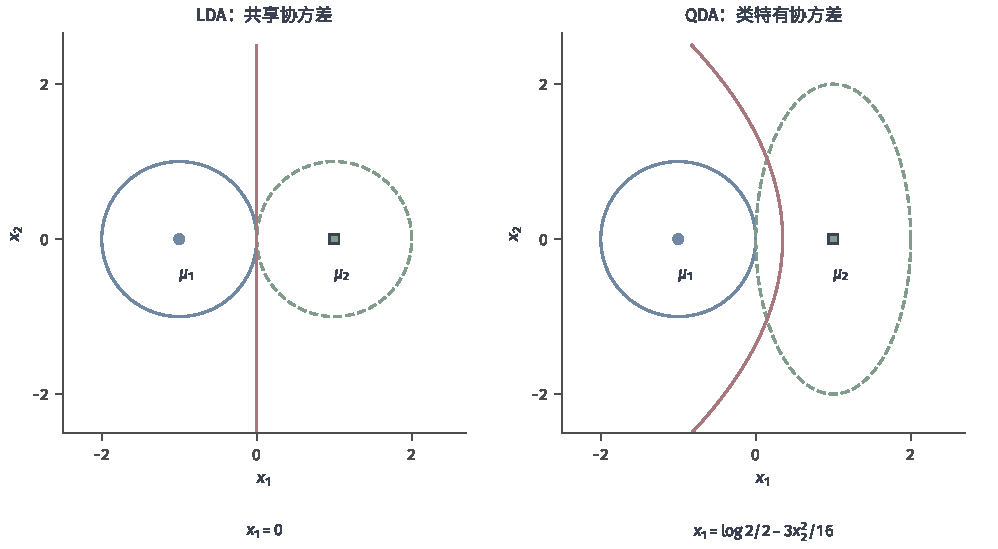
\includegraphics[width=159.059mm]{figures/04-classic-models/00-shared/matplotlib/classification-gaussian-boundaries/figure.pdf}
  \caption{两图均取$\pi_1=\pi_2=1/2$、$\bm{\mu}_1=(-1,0)^{\top}$、$\bm{\mu}_2=(1,0)^{\top}$和$\bm{\Sigma}_1=\bm{I}_2$，仅第2类协方差变化。蓝色圆点和绿色方点为均值，蓝色实线与绿色虚线分别为$\Delta_1=1$和$\Delta_2=1$的等密度轮廓；不同类的这些轮廓不保证密度值相同。红色粗线按$g_1=g_2$的解析式绘制，底部公式分别给出LDA的线性边界与QDA的二次边界。参数均为教学构造，不是采样或拟合结果。}
  \label{fig:classification-gaussian-boundaries}
\end{figure*}

对二分类，把式~\eqref{eq:classification-lda-score}~中的两类得分相减并归一化，就得到Logistic形式的后验。因此，共享高斯假设蕴含线性对数几率，反过来却不成立；许多非高斯输入分布也能有Logistic形式的条件概率。即便两条路线的后验形式相同，用联合似然估计均值和协方差，与直接最大化条件似然，也通常得到不同的有限样本参数。

完整协方差每类需要$d(d+1)/2$个自由参数。类内散布矩阵的秩至多为$n_c-1$，因而$n_c\leq d$时必然奇异，不能直接代入普通高斯密度；$n_c>d$也不保证估计准确或条件良好。共享估计的秩至多为$n-C$。在维数较大或类别样本少时，可以共享、取对角，或采用第\ref{sec:classification-lda-covariance-extensions}节的RDA收缩估计。式\eqref{eq:classification-rda}已经说明这些约束如何借用合并统计量和球形方差；使用收缩就改变了估计准则，不再是未经约束的MLE。

稠密完整协方差的统计成本约为$O(nd^2)$，各类矩阵分解约为$O(Cd^3)$，存储为$O(Cd^2)$，QDA单样本得分约为$O(Cd^2)$。LDA只需分解一份协方差，并可预先算出线性权重，使单样本预测降到$O(Cd)$。实现时可用Cholesky分解求解二次型与对数行列式，无须显式构造逆矩阵。

\subsection{模型对比与总结}
\label{sec:classification-probability-comparison}

Logistic与Softmax直接拟合类别条件概率，NB与GDA先拟合类先验和类条件输入分布。前者不必解释输入怎样产生，后者则可利用分布约束减少需要估计的关系。二分类Logistic是Softmax的两类形式；两者都以互斥类别为对象，多标签任务需要另行规定每个标签事件的模型。

高斯模型的关系由协方差约束决定：QDA允许各类独立的完整协方差，LDA要求共享，高斯NB要求各类协方差对角。LDA与高斯NB各自限制了不同对象，不能一般地按强弱排序。共享高斯模型的共同二次项在类别比较中相消，后验可写成线性Softmax；QDA则需要平方项和交叉项。为Softmax提供这些扩展特征可以表达QDA后验，却无需把系数解释为高斯密度参数。相同的后验形式也不意味着相同学习：联合似然估计与条件似然估计在有限样本上通常选出不同系数。

NB与线性Logistic的联系还取决于事件模型。参数严格为正时，伯努利NB的对数得分累加二值字段，多项式NB的得分按本节文档长度约定累加词项计数，其后验可以写成这些特征上的Softmax。高斯NB在各类单维方差不同时还含有平方项，只是没有跨坐标的交叉项。补集NB改变统计来源，AODE增加部分条件依赖；收缩协方差改变估计约束。这些变化应分别与具体数据缺口比较，不能一律解释成“概率模型更复杂”。

表\ref{tab:classification-probability-comparison}汇总相同监督分类任务下的主要取舍。参数量按每维分布参数有界计算，GDA的共享与类特有协方差分别列明，避免把两者的代价混在一起。
\begin{table}[htbp]
  \centering
  \small
  \begin{tabularx}{\linewidth}{@{}
    >{\RaggedRight\arraybackslash}p{0.19\linewidth}
    >{\RaggedRight\arraybackslash}X
    >{\RaggedRight\arraybackslash}X@{}}
    \toprule
    模型 & 建模与估计 & 主要取舍 \\
    \midrule
    Logistic回归／Softmax回归 &
    直接拟合条件概率；$O(Cd)$个参数，迭代优化 &
    不拟合输入分布；需检查特征表示、分离与正则化 \\
    NB &
    由先验和简化类条件模型形成后验；通常$O(Cd)$个参数 &
    计数或矩估计易累积；依赖和事件模型失配会引入偏差 \\
    共享GDA（LDA） &
    高斯类条件分布，共享协方差；$O(d^2+Cd)$个参数 &
    用共同协方差降低估计波动；只得到线性边界 \\
    类特有GDA（QDA） &
    各类独立估计协方差；$O(Cd^2)$个参数 &
    边界更灵活；对每类样本量和协方差条件更敏感 \\
    \bottomrule
  \end{tabularx}
  \caption{概率分类模型的建模对象与估计代价。所有概率输出都需单独检查校准，参数量不直接等于达到指定精度所需的样本量。}
  \label{tab:classification-probability-comparison}
\end{table}

类条件假设可以减轻小样本下的估计负担，也可能留下模型失配。Ng和Jordan对特定NB与判别式模型的研究展示了这种取舍，不能据此给全部生成式与判别式模型排序\scite{ng2001}。实际选择应固定输入表示、数据划分、误判代价和调参预算，比较分类错误、概率质量与计算成本；训练误差更小或输出取值合法，都不能单独说明概率已经可靠。

\section{基于集成的分类}
\label{sec:classification-ensemble}

集成可以组合硬标签、类别得分或概率，整体输出决定分类任务的使用方式。例如GBDT用回归树拟合类别得分的修正，再由累积得分形成类别决策；成员的数值输出与整体分类目标相容。下面比较各方法的输出、阈值和概率检验，成员组合的基本机制见第\ref{sec:classic-overview-ensemble}节，完整训练过程见第\ref{chap:ensemble-learning}章。

\begin{table*}[htbp]
  \centering
  \small
  \begin{tabularx}{\linewidth}{@{}>{\RaggedRight\arraybackslash}p{22mm}>{\RaggedRight\arraybackslash}X>{\RaggedRight\arraybackslash}X@{}}
    \toprule
    方法 & 分类输出 & 任务中的条件与代价 \\
    \midrule
    Bagging & 硬标签投票，或平均成员得分／概率后决策 & 概率平均不自动校准；预测成本随所用成员增加 \\
    随机森林 & 树投票或叶类别比例平均 & 树深、特征抽样与树数需选择；袋外诊断不替代测试 \\
    AdaBoost & 对弱分类器加权投票或输出累计得分 & 加权分类问题上的成员表现与噪声影响轮次选择 \\
    GBDT & 累加类别得分，再按阈值或Softmax决策 & 分类损失决定修正；树深、学习率与早停共同影响结果 \\
    Stacking & 元学习器组合标签、得分或概率 & 组合层用留出或折外基预测训练；校准仍需独立检验 \\
    \bottomrule
  \end{tabularx}
  \caption{集成方法的分类输出与使用条件。此处按分类输出与训练条件比较；成员训练机制见概述与集成学习章。}
  \label{tab:classification-ensemble-map}
\end{table*}

集成的投票和得分需要按整体预测评价。表\ref{tab:classification-evaluation-protocol}给出标签错误、排序、概率与误判代价的对应指标，资源成本计入实际使用的全部成员。组合后的概率质量和解释性由整体模型检验。对于奇数个二分类成员的等权多数投票，若在目标分布几乎所有输入与标签上，成员错误在给定输入与标签后关于训练随机性相互独立，且每个成员的条件错误率都至少比$1/2$小同一个正数，则平均训练随机性后的投票风险具有随成员数指数下降的上界。二分类AdaBoost的训练误差上界下降则需各轮保持带权优势，泛化还需投票间隔或基类容量控制（参考\BookSectionRef{sec:boosting}{卷3《基础、理论与可信性》第5章“二分类学习的可学习性”第5.6节“集成学习”}）。

\section{半监督分类}
\label{sec:classification-semisupervised}

前面介绍的分类器依靠带标签的样本选择决策边界，但能够收集到的输入往往多于能够完成标注的样本。例如，积累一批待分类文档相对容易，逐篇判断主题却需要人工阅读。如果只使用已经标注的少量文档，其余文档所反映的词语共现和主题聚集结构就没有参与学习。\term{半监督分类}（semi-supervised classification）试图利用这部分信息：由真实标签确定类别含义，再借助未标注输入约束预测规则。

本节把全部$n$个样本的索引分成不相交的有标签集合$L$与无标签集合$U$，满足$L\cup U=\{1,\dots,n\}$。每个输入为$\bm{x}_i\in\mathbb{R}^{d}$，只有$i\in L$时可以在训练中使用真实标签$y_i$；除二分类的专门约定外，类别取值为$\{1,\dots,C\}$。这里的“无标签”描述算法可用的信息，不表示样本在真实任务中没有类别。标签稀缺是学习条件，树、概率模型和间隔模型则描述怎样表示或学习分类规则，因而半监督方法可以与前面几节的模型组合使用。

输入结构与类别之间的联系决定未标注数据能提供什么帮助。同样的两团文档，可能对应两个主题，也可能只因写作风格不同而聚集。分布不匹配、标签采样偏差或未知类别混入，都可能使采用的结构假设失效。Cozman与Cohen对生成式分类器的分析表明，生成模型失配时，加入未标注数据可能增大渐近偏差和分类错误\scite{cozman2002unlabeled}。其结论限定于所分析的生成式模型，指出了核对结构假设的必要性。

Self-Training将筛选后的模型预测作为补充监督，Label Propagation沿相似关系平滑标签得分，TSVM利用输入密度选择间隔边界。三种机制可以共享条件，也可以组合。下面分别说明未标注输入怎样进入训练、目标怎样求解，以及哪些分布联系支撑样本外收益。

\subsection{Self-Training}
\label{sec:classification-self-training}

已经用少量标注文档训练出一个分类器以后，可以先让它预测其余文档。例如，模型对某些包含已知主题词的文档有较高置信度，而这些文档还包含原标注集中少见的其他词。若采纳的类别判断可靠，重新训练就能把这些新词与已有类别联系起来，扩展原来的标签覆盖。

\term{自训练}（self-training）将这个思路组织成外层循环：基分类器产生预测，外层策略筛选部分预测作为补充标签，再扩充训练集并重新拟合。它复用已有分类器，新增的是筛选与重训机制。高置信度也可能来自模型的错误偏好，后面需要检查采纳规则及错误反馈。用机器自身的输出代替部分教师信号的思想，在Scudder于1965年研究的自适应模式识别方法中已经出现；现代筛选、加权和重训方式则可以有许多实现\scite{scudder1965selftraining}。

\subsubsection{模型结构}
\label{sec:classification-self-training-structure}

自训练不要求一种新的决策边界形式。基分类器仍可采用Logistic回归、SVM、决策树或随机森林；新增的部分是怎样管理暂时没有真实标签的样本。为了不混淆真实监督与模型生成的监督，保持原始$L$和$U$不变，用$A^{(t)}\subseteq U$记录第$t$轮已经采纳伪标签的样本索引，用$R^{(t)}=U\setminus A^{(t)}$记录剩余候选池。初始时$A^{(0)}=\varnothing$，模型只在$L$上训练。

假设基分类器以参数$\bm{\theta}$给出类别概率估计$p_{\bm{\theta}}(c\mid\bm{x})$。本节讨论一种阈值筛选方式，把最大类别概率作为\term{置信度}（confidence），即模型对自己当前分类结果的确定程度。对$j\in R^{(t)}$，计算
\begin{equation}
  \label{eq:classification-self-training-selection}
  \begin{aligned}
    \widehat y_j^{(t)}
      &=\argmax_{1\leq c\leq C}
        p_{\bm{\theta}^{(t)}}(c\mid\bm{x}_j),\\
    q_j^{(t)}
      &=\max_{1\leq c\leq C}
        p_{\bm{\theta}^{(t)}}(c\mid\bm{x}_j),\\
    B^{(t)}
      &=\{j\in R^{(t)}:q_j^{(t)}\geq\tau\}.
  \end{aligned}
\end{equation}
其中$\tau$是预先选择的阈值，通常取$1/C<\tau<1$；遇到并列最大值时，本节统一取编号最小的类别。被采纳的预测$\widetilde y_j=\widehat y_j^{(t)}$称为\term{伪标签}（pseudo-label）：它是模型提出的临时训练目标，并没有经过真实标注确认。本节的基本版本在采纳后固定该标签；允许重估或撤销伪标签的版本需要另外规定更新规则。

概率阈值要求筛选分数具有概率含义。SVM得分需先用独立标注数据建立并检验概率映射；直接输出概率的模型也需检查高置信度样本的实际错误率。例如二分类预测$(0.96,0.04)$满足$\tau=0.9$，$(0.55,0.45)$则被保留在候选池。采纳的是模型判为可靠的预测，真实标签仍待另行确认。

\subsubsection{参数学习}
\label{sec:classification-self-training-learning}

每轮采纳伪标签后，基分类器需要重新拟合。以可加权的损失$\ell$为例，当前训练目标可以写成
\begin{equation}
  \label{eq:classification-self-training-objective}
  \begin{aligned}
    \mathcal{J}_t(\bm{\theta})
      ={}&\frac{1}{|L|}\sum_{i\in L}
        \ell\bigl(f_{\bm{\theta}}(\bm{x}_i),y_i\bigr)\\
      &+\frac{\eta}{\max\{1,|A^{(t)}|\}}
        \sum_{j\in A^{(t)}}
        \ell\bigl(f_{\bm{\theta}}(\bm{x}_j),\widetilde y_j\bigr)\\
      &+\beta\Omega(\bm{\theta}).
  \end{aligned}
\end{equation}
这里$L$非空，$\eta\geq0$控制伪标签项的相对权重，$\beta\Omega$沿用基分类器的正则化方式。空伪标签集的求和取零。分别归一化两类样本，是为了避免仅因伪标签数量增加就让它们压过真实标签；若采用统一样本权重，其相对影响会随集合大小改变。对于树等不直接求解这个目标的分类器，可以使用对应的带权拟合接口，自训练的集合更新逻辑不变。

算法\ref{alg:classification-self-training}给出固定阈值、固定已采纳伪标签的版本。$\operatorname{Fit}(A)$表示用真实标签集与索引为$A$的伪标签集完成一次基分类器训练，并返回参数；式~\eqref{eq:classification-self-training-objective}~是这种训练的一种具体实现。算法中省略集合的迭代上标，始终让当前参数对应当前已采纳的训练集。

\begin{algorithm}[带最终重训的自训练]
  \label{alg:classification-self-training}
  \begin{algorithmic}[1]
    \Require 有标签索引$L$、无标签索引$U$及其输入
    \Require 阈值$\tau$、最大扩充轮数$T\geq0$
    \Ensure 分类器$f_{\bm{\theta}}$、已采纳索引$A$和剩余索引$R$
    \State $A\gets\varnothing$，$R\gets U$
    \State $\bm{\theta}\gets\operatorname{Fit}(A)$
    \For{$t=1,\dots,T$}
      \If{$R=\varnothing$}
        \State \textbf{break}
      \EndIf
      \State 用当前模型计算$R$中的$\widehat y_j$与$q_j$
      \State $B\gets\{j\in R:q_j\geq\tau\}$
      \If{$B=\varnothing$}
        \State \textbf{break}
      \EndIf
      \State 保存$\widetilde y_j\gets\widehat y_j$，$j\in B$
      \State $A\gets A\cup B$，$R\gets R\setminus B$
      \State $\bm{\theta}\gets\operatorname{Fit}(A)$
    \EndFor
    \State \Return $f_{\bm{\theta}},A,R$
  \end{algorithmic}
\end{algorithm}

把重训放在集合扩充之后有一个直接作用：无论这一轮恰好用完最大轮数，还是把剩余池清空，返回的模型都已经使用了本轮加入的伪标签。若把训练放在循环开头、随后只添加样本就退出，最后一批伪标签实际上不会影响返回模型。预测前检查空池也很必要，空输入未必被基分类器的批量预测接口接受。当$U$为空或$T=0$时，算法自然返回纯监督模型。

图\ref{fig:classification-self-training}中的反馈箭头将重训后的模型送回预测步骤。真实标签固定在$L$中，未采纳的样本保留在$R$，已采纳的预测保存在$A$；这些集合变化记录监督的来源，使每轮能够区分真实标签与模型生成的伪标签。

\begin{figure*}[htbp]
  \centering
  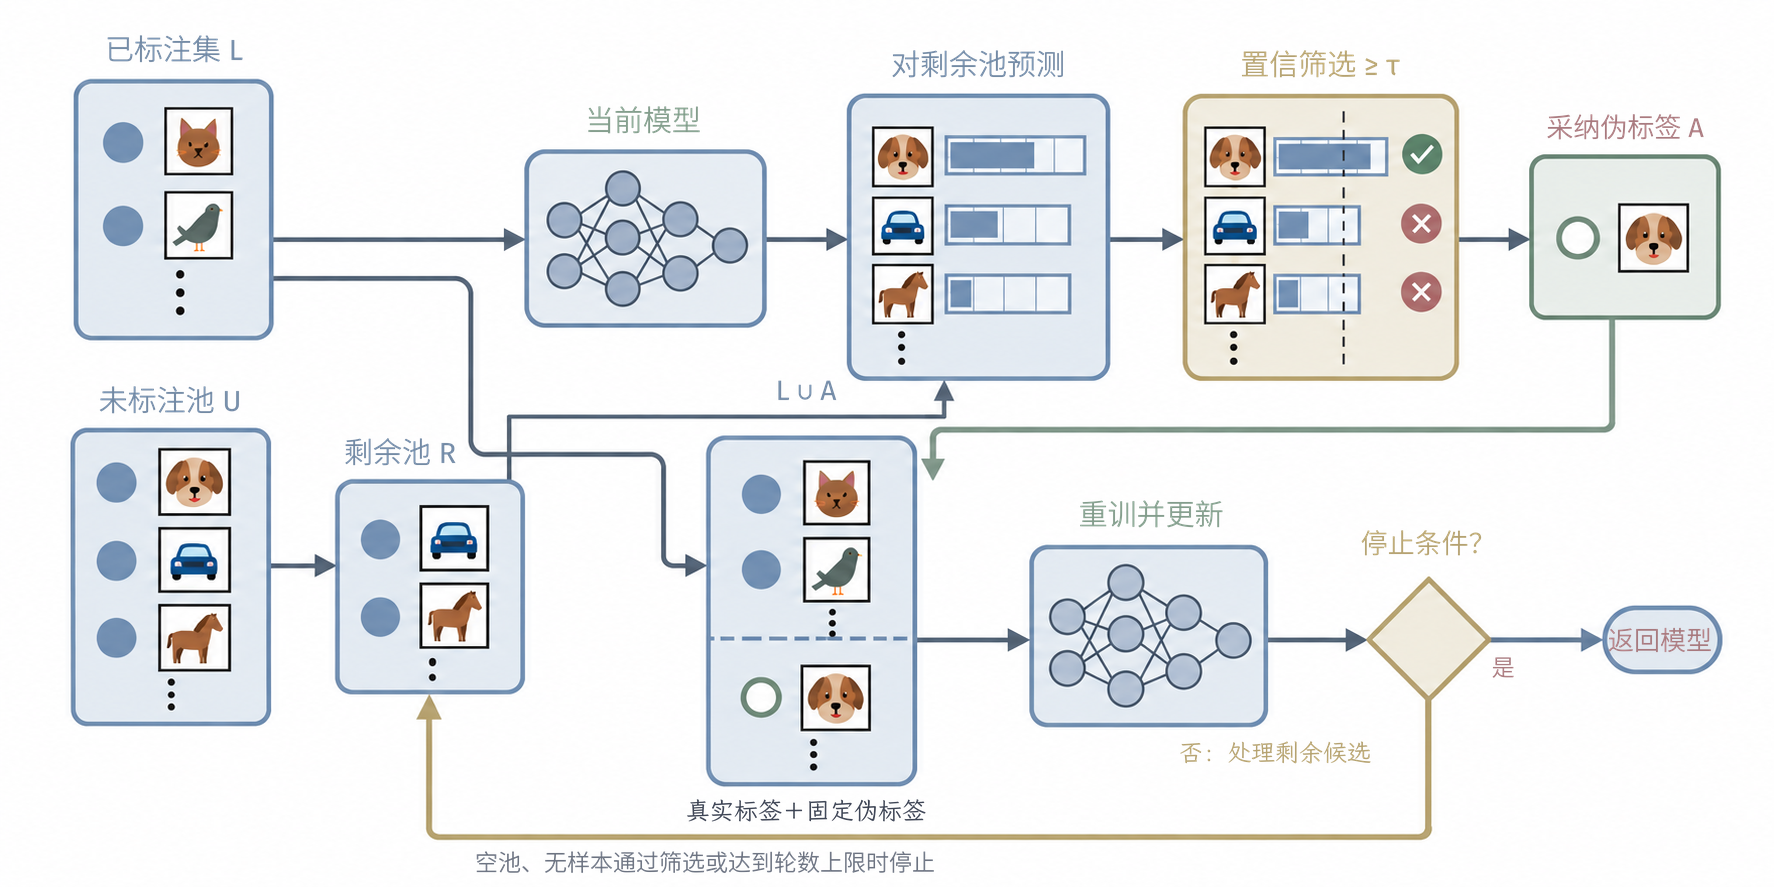
\includegraphics[width=150.199mm]{figures/04-classic-models/00-shared/generated/classification-self-training/figure.png}
  \caption{固定阈值、固定已采纳伪标签的自训练流程，对应算法~\ref{alg:classification-self-training}。真实标签保持不变，已采纳的伪标签始终是模型预测。每次采纳后先重训，再用更新后的模型处理剩余候选；空池、无样本通过筛选或达到轮数上限时停止。这个模型反馈回路也可能产生确认偏差：错误预测被当作后续监督，使模型进一步强化原有误判。}
  \label{fig:classification-self-training}
\end{figure*}

每轮也可以在通过阈值的样本中只取前若干项，限制一次扩充的影响；按类别限制数量则可避免易预测类别占据全部新增监督。这些策略改变$B^{(t)}$的构造，集合更新仍按保存标签、扩充集合、重训的顺序执行。类别配额依据任务中的类别比例设置。

\subsubsection{理论分析}
\label{sec:classification-self-training-analysis}

\paragraph{表达能力}
自训练沿用基分类器的特征与函数形式，候选类不会因增加伪标签而扩大。若基分类器只使用原坐标的仿射得分，前面的四点异或仍不能精确表示，等概率四点上的标签不一致比例至少为$1/4$。加入$x_1x_2$后，得分$-x_1x_2$才使这项目标进入候选类。

\paragraph{收敛性}
这个基本版本何时停止，可以直接从集合变化判断。每次成功扩充至少从$R$移走一个样本，且样本不会移回，因此成功扩充最多发生$\min\{T,|U|\}$次；若没有样本通过筛选，循环会更早结束。只要每次基分类器训练能够返回，外层循环就会有限终止。这一保证针对集合扩充过程的有限终止；各轮训练集和监督信号发生变化，参数优化与统计风险需针对相应模型另行分析。

自训练与\term{熵最小化}（entropy minimization）有共同的倾向：都可能让未标注样本上的预测变得更确定。熵最小化直接惩罚模型预测分布的条件熵，推动概率集中到少数类别。Grandvalet与Bengio讨论了这一准则及其与自训练的联系，这种联系依赖具体的概率模型、筛选和优化设置\scite{grandvalet2004entropy}。

对一个未标注输入$\bm{x}$，Shannon熵与硬伪标签交叉熵分别涉及
\begin{equation}
  \label{eq:classification-pseudolabel-entropy}
  \begin{aligned}
    H_{\bm{\theta}}(\bm{x})
      &=-\sum_{c=1}^{C}p_{\bm{\theta}}(c\mid\bm{x})
        \log p_{\bm{\theta}}(c\mid\bm{x}),\\
    \min_{\widetilde y\in\{1,\dots,C\}}
      \{-\log p_{\bm{\theta}}(\widetilde y\mid\bm{x})\}
      &=-\log\max_c p_{\bm{\theta}}(c\mid\bm{x}).
  \end{aligned}
\end{equation}
前者对所有类别求加权和，后者只取概率最大的一个类别，两者数值和梯度一般不同。例如，预测为$(0.8,0.2)$时，以自然对数计算的熵约为$0.500$，最小硬标签交叉熵约为$0.223$。实际自训练还会筛选样本并冻结历史伪标签，因此下一轮甚至不一定仍以当前最大概率类别为目标。

\paragraph{泛化性}
在同一聚集区域内限制预测差异时，熵最小化倾向于同时提高这些输入的确定性，使边界远离该区域；具体效果依赖基分类器的容量与约束方式。确定性本身仍只描述概率集中程度：若初始模型把同主题文档误判为另一类，采纳后重训可能加强原误判。这种自身错误被重复用作监督的现象称为\term{确认偏差}（confirmation bias）。Arazo等在深度图像分类实验中观察到错误伪标签被拟合，并比较了缓解这一反馈的正则化方法\scite{arazo2020confirmation}。

伪标签错误怎样影响真实风险，可以在固定一轮模型后直接推导。令$h$为这一轮产生伪标签的分类器，$\bm{X}_\tau\subseteq\mathbb{R}^{d}$为通过其置信度阈值的输入区域；$R_{\mathcal P}$沿用目标分布上的零一风险记号。设$\pi=\mathbb{P}_{\mathcal{P}}(\bm{x}\in\bm{X}_\tau)>0$，在筛选区域内分别考察伪标签自身的错误率，以及$f$与伪标签不一致的概率：
\begin{equation}
  \label{eq:classification-self-training-conditional-risks}
  \begin{aligned}
    e_\tau
      &=\mathbb{P}_{\mathcal{P}}
        \bigl(h(\bm{x})\ne y\mid\bm{x}\in\bm{X}_\tau\bigr),\\
    \widetilde R_\tau(f)
      &=\mathbb{P}_{\mathcal{P}}
        \bigl(f(\bm{x})\ne h(\bm{x})\mid\bm{x}\in\bm{X}_\tau\bigr).
  \end{aligned}
\end{equation}
若$f$预测错误，它要么与$h$不一致，要么沿用了$h$的错误，因此
\begin{equation}
  \label{eq:classification-self-training-error-events}
  \{f(\bm{x})\ne y\}
    \subseteq
    \{f(\bm{x})\ne h(\bm{x})\}
    \cup\{h(\bm{x})\ne y\},
\end{equation}
在$\bm{X}_\tau$内应用并集界，再把区域内外的风险相加，得到
\begin{equation}
  \label{eq:classification-self-training-risk}
  \begin{aligned}
    R_{\mathcal{P}}(f)
      \leq{}&\pi\bigl(\widetilde R_\tau(f)+e_\tau\bigr)\\
      &+\mathbb{P}_{\mathcal{P}}
        \bigl(f(\bm{x})\ne y,\ \bm{x}\notin\bm{X}_\tau\bigr).
  \end{aligned}
\end{equation}
式~\eqref{eq:classification-self-training-risk}中的$\widetilde R_\tau(f)$仍是期望不一致损失，不能用训练伪标签上的错误直接替换。若产生标签的模型与新输入池独立，可以把这一步也写成风险界。
\begin{theorem}[自训练在独立输入池与固定候选类下的期望风险界]
  \label{thm:classification-self-training-risk}
  条件于已经训练好的$h$，固定筛选区域$\bm X_\tau$，并在采集本轮伪标签输入前固定含$N\geq1$个分类器的候选类$\mathcal F$。独立抽取$m\geq1$个来自$P_X(\cdot\mid\bm X_\tau)$的输入，以$h$的预测为标签。学习器用这些样本和已有监督返回$\hat f\in\mathcal F$，记其本轮伪标签训练错误为
  \[
    \widehat R_{\mathrm{pseudo}}(\hat f)
      =\frac1m\sum_{j=1}^m
        \mathbb1\{\hat f(\bm x_j)\ne h(\bm x_j)\}.
  \]
  对$0<\delta<1$，关于本轮输入抽样，至少以$1-\delta$的概率，
  \[
    R_{\mathcal P}(\hat f)
      \leq\pi\left[
        \widehat R_{\mathrm{pseudo}}(\hat f)+e_\tau
        +\sqrt{\frac{\log(2N/\delta)}{2m}}\right]
       +(1-\pi).
  \]
\end{theorem}
\begin{proof}
  固定$h$以后，与其伪标签不一致的损失取值于$[0,1]$，其期望是$\widetilde R_\tau(f)$。对本轮独立样本和预定候选类使用有限类的一致偏差界，得到
  $\widetilde R_\tau(\hat f)\leq\widehat R_{\mathrm{pseudo}}(\hat f)
       +\sqrt{\log(2N/\delta)/(2m)}$。
  代入式\eqref{eq:classification-self-training-risk}，再用$1-\pi$上界区域外错误，即得结论。
\end{proof}

这说明即使重训模型完全拟合伪标签，仍要保留采纳区域中的真实错误$e_\tau$和区域外风险。较高的概率阈值本身不提供$e_\tau$的上界；它需要可靠的概率条件或独立真实标签来支持。定理分析的是一轮固定教师、独立输入池和有限候选类；连续参数基模型需要相应容量界。多轮使用同一输入池时，历史伪标签来自不同模型与采纳事件，不能把累积伪标签数直接当作这里的独立样本数$m$。

提高阈值减少采纳量，系统性的高置信度错误仍可能被保留。伪标签权重与单轮规模控制其训练影响，逐类接受率揭示扩充偏向，保留的真实标签验证集则比较扩充前后的效果。验证样本应独立于反复采纳的训练池。未知类别或监督样本覆盖不足时，还需检查数据组成与筛选区域是否符合任务。

\subsubsection{优化泛化能力}

\paragraph{保留未标注类别的不确定性}
\label{sec:classification-self-training-soft-em}

自训练将筛选后的类别作为确定标签；若基分类器已经建立NB或高斯类条件分布，还可以保留类别的不确定性，改用联合似然组织训练。例如，一篇文档当前可能有较高概率属于科技，也有一定概率属于文化，与其立即固定成科技类，不如按两类的后验权重分配它的词频贡献，并在参数更新后重新计算归属。这是生成式半监督方法用潜类别与EM利用未标注输入的路线。它与筛选硬伪标签的自训练使用不同训练目标，不是简单地把筛选阈值调低。

设联合模型为$p_{\bm{\theta}}(\bm{x},y)$，有标签样本直接贡献输入与类别的联合对数似然，未标注样本则只贡献输入的边缘对数似然：
\[
  \ell(\bm{\theta})
  =\sum_{i\in L}\log p_{\bm{\theta}}(\bm{x}_i,y_i)
   +\sum_{j\in U}\log\sum_{c=1}^{C}
      p_{\bm{\theta}}(\bm{x}_j,c).
\]
在这个模型中，全部输入与全部类别合称\term{完全数据}（complete data），其中包括实际未观测的类别；这里的“完全”指连同潜类别一并规定的随机变量。EM在训练时把$U$中的未知类别作为潜变量处理。E步用当前参数计算软后验$q_j(c)=p_{\bm{\theta}^{(t)}}(y=c\mid\bm{x}_j)$；M步最大化当前软后验下的期望完全数据对数似然。记
\[
  \begin{aligned}
    Q(\bm{\theta}\mid\bm{\theta}^{(t)})
    &=
    \sum_{i\in L}\log p_{\bm{\theta}}(\bm{x}_i,y_i) \\
    &\quad+
    \sum_{j\in U}\sum_{c=1}^{C}
      q_j(c)\log p_{\bm{\theta}}(\bm{x}_j,c), \\
    \bm{\theta}^{(t+1)}
    &\in\argmax_{\bm{\theta}}
      Q(\bm{\theta}\mid\bm{\theta}^{(t)}).
  \end{aligned}
\]
只有对多项式NB这类以类别与类别词频为充分统计量的模型，M步才可以解释为把$q_j(c)$作为分数类别计数，与真实标签统计量一起更新先验和类条件参数。此时，未标注文档的词频按$q_j(c)$分配给各类别，而不是先固定成一个不可更改的硬伪标签。Nigam等在文本分类中给出了这一路线的代表性实现\scite{nigam2000text}。

EM改变估计过程，联合分布仍限于预定的$p_{\bm\theta}(\bm x,y)$。选多项式NB就仍使用加性的词频证据，选每类单个高斯就仍不能表达任意多峰类内分布；未标注数据不会替模型补上缺少的依赖项。分布族能够表达真实联合分布时，软类别统计量才有对应的目标参数；这与EM是否找到全局似然最大点仍是两个问题。

模型失配时，大量未标注输入可能加强对错误边缘结构的拟合；Cozman与Cohen对分类性能劣于监督基线的现象给出了分析与实验\scite{cozman2002unlabeled}。后验不能闭式计算时，近似推断又增加了一层误差与计算选择；相应图模型入口见\BookVolumeRef{vol:probabilistic-graphical-models}{卷六“模型：概率图模型”}。

\paragraph{降低伪标签对单个教师的依赖}
同一个模型提出并采纳标签时，系统性偏差可能被重复使用。若输入具有两种各自足以分类的描述，Blum与Mitchell在1998年提出的\term{协同训练}（co-training）可以让两个视图的分类器互供候选标签；其理论设定还要求给定类别后的视图条件独立。没有这种视图关系时，互供标签也可能传播共同错误，且需要训练和评价两个模型\scite{blum1998cotraining}。

没有两种天然视图时，Zhou与Li在2005年提出的\term{三训练}（tri-training）用重采样初始化三个模型，让两个模型的一致预测为第三个提供候选标签，并控制新增标签的错误负担。这增加了模型训练和预测成本，一致意见是否有用仍取决于错误相关性；它改变了监督来源，不是单模型自训练的一项默认设置\scite{zhou2005tritraining}。

\subsubsection{小结}
\label{sec:classification-self-training-summary}

自训练把已有分类器的部分预测转化为新增监督，适合在保留原有训练和预测接口的情况下探索无标签数据的价值。它的额外成本包括对剩余池反复预测，以及在不断扩大的训练集上重新拟合；基分类器训练昂贵时，这些成本并不小。最终模型仍按原分类器的方式预测新样本，无须保留一个独立的传播图。

硬伪标签把当前判断作为后续监督，生成式EM则按当前软类别归属分配统计量，并反复更新联合模型。前者依赖筛选是否可靠，后者还依赖输入分布是否被模型正确描述；两者都可能把错误结构反复写入训练。保留真实标签验证集和针对高代价样本的人工复核，有助于判断新增监督是否值得采纳。

互供标签改变的是新增监督从哪里来。协同训练依靠不同视图，三训练依靠多个模型的一致判断；它们需要更多模型的训练和预测，也要检查共同错误是否被反复采纳。软类别归属与多模型监督来源因此是两个可以分别考虑的方向，不构成由简单到复杂的性能排序。

\subsection{Label Propagation}
\label{sec:classification-label-propagation}

自训练通过基分类器决定哪些预测值得采纳；如果可信的信息主要来自样本之间的邻近关系，也可以直接在这些关系上传递标签。\term{标签传播}（label propagation）把样本表示为图的节点，让已有标签沿相似边影响尚无标签的节点。Zhu与Ghahramani在2002年的技术报告中给出了保持已知标签不变的传播方法\scite{zhu2002labelpropagation}。与只在已标注样本中寻找近邻相比，未标注点也参与形成传播路径，使标签能够沿弯曲的高密度区域传递；每轮恢复已知标签，则让它们持续提供监督，不会因反复平均而失去原有的类别信息。

下面用随机游走解释固定标签边界下的传播，软约束版本随后通过另一目标引入。

\subsubsection{模型结构}
\label{sec:classification-label-propagation-structure}

图模型把“哪些输入相似”转化成可计算的边权。令$\mathcal{G}=(V,E,\bm{W})$，其中$V=L\cup U$，$\bm{W}\in\mathbb{R}^{n\times n}$为非负对称权重矩阵，$\bm{W}_{i,j}=\bm{W}_{j,i}\geq0$，且取$\bm{W}_{i,i}=0$。例如，可以先选出近邻边，再在相连节点上使用RBF相似度
\begin{equation}
  \label{eq:classification-label-propagation-weights}
  \bm{W}_{i,j}=
  \begin{cases}
    \exp\bigl(-\gamma\lVert\bm{x}_i-\bm{x}_j\rVert_2^2\bigr),
      & \{i,j\}\in E,\\
    0, & \text{其他情形},
  \end{cases}
\end{equation}
其中$\gamma>0$控制相似度衰减。用$k$近邻关系构图时，单向近邻关系需要经过并集或互近邻等明确规则转成无向边，才能满足对称性。完全图保留所有样本对，稀疏图只保留选中的关系；两者不仅存储成本不同，也可能给出不同的分类结果。

每个节点的加权度记为$\delta_i=\sum_j\bm{W}_{i,j}$，度矩阵满足$\bm{D}_{i,i}=\delta_i$。在所有参与传播的节点度数为正时，定义
\begin{equation}
  \label{eq:classification-label-propagation-transition}
  \bm{P}=\bm{D}^{-1}\bm{W},
  \qquad
  \bm{P}_{i,j}=\frac{\bm{W}_{i,j}}{\delta_i}.
\end{equation}
矩阵$\bm{P}$每行的和为1，表示从一个节点沿边随机走向邻居的转移概率。传播时用这一行权重对邻居的标签信息求平均；权重大，邻居的影响也大。

为了同时处理$C$个类别，令$\bm{F}\in\mathbb{R}^{n\times C}$保存节点得分，$\bm{f}_i=(\bm{F}_{i,1},\dots,\bm{F}_{i,C})^\top$为节点$i$的得分向量。构造同形状的$\bm{Y}$：若$i\in L$，则$\bm{Y}_{i,c}=\mathbb{1}\{y_i=c\}$；若$i\in U$，则整行置零。有标签节点在每轮更新后都恢复到这份独热编码，这种固定边界的操作称为\term{硬钳制}（hard clamping），也就是不允许传播改变已经给定的标签。

标签边界应能沿图到达每个待预测节点。零度无标签节点没有转移概率，完全无标签的连通分量则缺少类别语义；可补充真实标签、按可靠关系重新构图，或对相应节点拒绝预测。孤立的有标签节点保留原标签。自环或微小度数只能调整数值形式，类别信息仍需要标签边界提供。

\subsubsection{参数学习}
\label{sec:classification-label-propagation-learning}

标签传播没有固定维数的分类器参数要拟合，但需要求出全部无标签节点的得分。下面假设零度节点已经处理，每个含无标签节点的连通分量至少含一个有标签节点。把$\bm{F}$按$L$与$U$分成行块$\bm{F}_L=\bm{F}_{L,:}$、$\bm{F}_U=\bm{F}_{U,:}$，并对$\bm{P}$作对应分块。硬钳制意味着$\bm{F}_L^{(t)}=\bm{Y}_L$始终不变，因而只需迭代
\begin{equation}
  \label{eq:classification-label-propagation-iteration}
  \bm{F}_U^{(t+1)}
    =\bm{P}_{U,U}\bm{F}_U^{(t)}
     +\bm{P}_{U,L}\bm{Y}_L.
\end{equation}
右侧第一项传递尚无标签节点之间的当前信息，第二项持续注入真实标签。通常取$\bm{F}_U^{(0)}=\bm{0}$。真实标签在每轮固定为边界，无标签行按该转移式更新。

若迭代达到固定点，移项便得到线性系统与形式上的闭式解
\begin{equation}
  \label{eq:classification-label-propagation-solution}
  \begin{aligned}
    (\bm{I}-\bm{P}_{U,U})\bm{F}_U^\ast
      &=\bm{P}_{U,L}\bm{Y}_L,\\
    \bm{F}_U^\ast
      &=(\bm{I}-\bm{P}_{U,U})^{-1}
        \bm{P}_{U,L}\bm{Y}_L.
  \end{aligned}
\end{equation}
这里$\bm{I}$为$|U|\times|U|$单位矩阵。本节理论分析将证明，在上述图条件下逆矩阵存在，且任意初始化的迭代都收敛到同一个解。计算时通常直接求解线性系统，避免显式构造逆矩阵。Zhu、Ghahramani与Lafferty给出了这一解的调和函数、图能量和随机游走解释\scite{zhu2003}。

图\ref{fig:classification-label-propagation}给出一个可逐项核算的教学构造，并非实测数据。五个节点依次相连，每条无向边的权重为1；端点1固定属于类1，端点5固定属于类2，节点2、3、4没有标签。令$p_i=\bm{F}_{i,1}^\ast$，由于每个内点恰有两个等权邻居，式~\eqref{eq:classification-label-propagation-iteration}~在固定点处变为
\begin{equation}
  \label{eq:classification-label-propagation-path}
  \begin{aligned}
    p_i&=\frac{p_{i-1}+p_{i+1}}{2},
      &&i=2,3,4,\\
    p_1&=1,\qquad p_5=0.
  \end{aligned}
\end{equation}
内点方程等价于$p_{i+1}-p_i=p_i-p_{i-1}$，所以相邻节点的得分差必须相等。两端总共下降1，分到四条边上，每步下降$1/4$，得到
\[
  (p_1,p_2,p_3,p_4,p_5)
    =(1,0.75,0.5,0.25,0).
\]
类2的得分满足相反的端点条件，故$\bm{f}_i^\ast=(p_i,1-p_i)^\top$。节点2偏向类1，节点4偏向类2；节点3的两类得分相同，按本节“并列时取最小类别编号”的约定判为类1。节点3的类别由并列规则确定，其两类得分所包含的证据仍相同。

\begin{figure}[htbp]
  \centering
  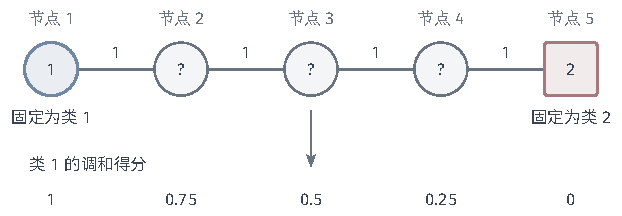
\includegraphics[width=105.315mm]{figures/04-classic-models/00-shared/tikz/classification-label-propagation/figure.pdf}
  \caption{五节点等权无向路径上的硬钳制标签传播。每条边权为1，左端圆形节点固定为类1，右端方形节点固定为类2，问号表示未知标签。下方列出精确调和解的类1得分，类2得分为其补数；内点得分等于两侧邻居的平均。中间节点两类并列，按最小类别编号规则判为类1。这是教学构造，不是实测结果。}
  \label{fig:classification-label-propagation}
\end{figure}

迭代实现还需要把停止条件与返回值对应起来。算法\ref{alg:classification-label-propagation}使用相邻两轮之差作为数值停止判据，其中$\lVert\cdot\rVert_{\mathrm{F}}$为Frobenius范数，$\varepsilon>0$为容限，$T\geq1$为最大迭代次数。达到上限时若尚未满足容限，返回状态记录为未收敛，以便解释当前得分的数值精度。

\begin{algorithm}[硬钳制标签传播]
  \label{alg:classification-label-propagation}
  \begin{algorithmic}[1]
    \Require 权重$\bm{W}$、索引$L,U$、标签矩阵$\bm{Y}$
    \Require 容限$\varepsilon>0$、最大迭代次数$T\geq1$
    \Ensure 得分$\bm{F}$、预测$\widehat{\bm{y}}_U$及停止状态
    \If{$U=\varnothing$}
      \State \Return $\bm{Y}$、空预测、已完成
    \EndIf
    \State 检查$\bm{W}$非负、对称，参与传播的节点度数为正
    \State 检查每个含$U$节点的连通分量至少有一个$L$节点
    \If{任何检查失败}
      \State \Return 拒绝结果，要求补标签或修正传播图
    \EndIf
    \State 构造$\bm{P}=\bm{D}^{-1}\bm{W}$
    \State $\bm{F}_L\gets\bm{Y}_L$，$\bm{F}_U\gets\bm{0}$
    \State $\mathrm{converged}\gets\mathrm{false}$
    \For{$t=1,\dots,T$}
      \State $\bm{G}\gets\bm{P}_{U,U}\bm{F}_U+\bm{P}_{U,L}\bm{Y}_L$
      \State $\Delta\gets\lVert\bm{G}-\bm{F}_U\rVert_{\mathrm{F}}$
      \State $\bm{F}_U\gets\bm{G}$
      \If{$\Delta\leq\varepsilon(1+\lVert\bm{F}_U\rVert_{\mathrm{F}})$}
        \State $\mathrm{converged}\gets\mathrm{true}$
        \State \textbf{break}
      \EndIf
    \EndFor
    \State $\widehat y_j\gets\argmax_c\bm{F}_{j,c}$，$j\in U$；并列取最小$c$
    \State \Return $\bm{F},\widehat{\bm{y}}_U,\mathrm{converged}$
  \end{algorithmic}
\end{algorithm}

算法先把$\bm{G}$保存成最新的$\bm{F}_U$，再判断是否退出，因此即使本轮达到容限，也会返回新得分而不是上一轮的值。相邻迭代差小是一种可操作的停止指标，不直接给出距离精确解的统一误差界；当传播很慢时，还需结合线性系统残差与条件数判断数值精度。最终类别由得分比较决定，接近平局的节点尤其需要保留得分与未收敛状态。

\subsubsection{理论分析}
\label{sec:classification-label-propagation-analysis}

\paragraph{表达能力}
固定图与标签边界时，硬钳制传播的候选得分须满足离散调和条件：标签节点保留给定得分，每个无标签节点的得分等于邻居得分的加权平均。若每个连通分量的真实类别都相同，且给定标签均正确，相应的常值独热得分就满足全部条件，目标因此在这个候选集合中，即使这些分量在原坐标中弯曲。

强连接中的交替标签则可能无法表达。例如，四个节点按$0,1,2,3$组成单位边权路径，节点0的标签为类1、节点3为类2。调和条件迫使两个内部节点的类2得分分别为$1/3$与$2/3$。按最大得分取类，它们只能分别归为类1和类2；若目标类别沿路径依次为1、2、1、2，两个内部节点便都与目标不一致。这一差距来自调和约束，目标所需的交替变化不在候选得分中。

\paragraph{收敛性}
硬钳制传播的收敛来自无标签节点能够沿正权路径到达标签边界。$\bm{P}_{U,U}$的行和至多为1，只有无标签邻居的节点其行和恰为1。因此考察多步后仍留在$U$中的总权重，可以同时处理直接与间接相连的节点。

\begin{theorem}[标签传播在各连通分量有标签条件下解的唯一性]
  \label{thm:classification-label-propagation-convergence}
  设图有限、边权非负且对称，所有参与传播的节点度数为正，$U$非空，且每个含无标签节点的连通分量至少含一个有标签节点。则$\rho(\bm{P}_{U,U})<1$，其中$\rho$表示谱半径。式~\eqref{eq:classification-label-propagation-iteration}~从任意初始得分出发，都收敛到式~\eqref{eq:classification-label-propagation-solution}~中的唯一固定点。
\end{theorem}

\begin{proof}
  从每个$j\in U$出发，选择一条到达$L$的正权路径，并在首次到达$L$时停止。有限图中这些路径长度有一个共同上界$m$，沿各路径行走的概率均为正，其最小值记为$\epsilon>0$。于是，无论从哪个无标签节点出发，在$m$步以内命中$L$的概率都至少为$\epsilon$。这说明
  \[
    \lVert\bm{P}_{U,U}^{m}\rVert_\infty\leq1-\epsilon,
    \qquad
    \rho(\bm{P}_{U,U})^m\leq1-\epsilon<1.
  \]
  因而$\bm{P}_{U,U}^t$趋于零，Neumann级数收敛，且
  \[
    (\bm{I}-\bm{P}_{U,U})^{-1}
      =\sum_{t=0}^{\infty}\bm{P}_{U,U}^{t}.
  \]
  迭代展开为
  \[
    \bm{F}_U^{(t)}
      =\bm{P}_{U,U}^{t}\bm{F}_U^{(0)}
       +\sum_{s=0}^{t-1}
         \bm{P}_{U,U}^{s}\bm{P}_{U,L}\bm{Y}_L.
  \]
  第一项消失，第二项趋于所述固定点。逆矩阵存在，也排除了其他固定点。
\end{proof}

还可以从最优化的角度解释同一个解。相邻节点的得分差越大，图上的不平滑程度越高。令$\bm{L}_{\mathrm{g}}=\bm{D}-\bm{W}$为\term{图拉普拉斯矩阵}（graph Laplacian），它把这种局部差异汇总成二次型。固定真实标签边界后，求解的\term{Dirichlet能量}（Dirichlet energy）最小化问题为
\begin{equation}
  \label{eq:classification-label-propagation-energy}
  \begin{aligned}
    \min_{\bm{F}:\,\bm{F}_L=\bm{Y}_L}\quad
    \mathcal{E}(\bm{F})
      &=\frac12\sum_{i,j=1}^{n}
        \bm{W}_{i,j}\lVert\bm{f}_i-\bm{f}_j\rVert_2^2\\
      &=\operatorname{tr}
        (\bm{F}^{\top}\bm{L}_{\mathrm{g}}\bm{F}).
  \end{aligned}
\end{equation}
第\ref{sec:clustering-spectral}节的谱聚类与第\ref{sec:dim-le}节的拉普拉斯特征映射复用图拉普拉斯和谱工具，但输出分别是离散簇分配与连续低维坐标；这里的标签传播则在已知类别语义下求类别得分。三种任务分别对类别得分、簇分配和坐标施加输出约束。

有标签节点固定为边界，优化变量只包含无标签行。对未知行块求导并令其为零，得到
\begin{equation}
  \label{eq:classification-label-propagation-dirichlet}
  \begin{aligned}
    (\bm{L}_{\mathrm{g}})_{U,U}\bm{F}_U
      &=-(\bm{L}_{\mathrm{g}})_{U,L}\bm{Y}_L\\
      &=\bm{W}_{U,L}\bm{Y}_L.
  \end{aligned}
\end{equation}
因为$(\bm{L}_{\mathrm{g}})_{U,U}=\bm{D}_{U,U}-\bm{W}_{U,U}$，左乘$\bm{D}_{U,U}^{-1}$就回到式~\eqref{eq:classification-label-propagation-solution}~的线性系统。

这个驻点也是唯一最小值，而不只是一个形式上的导数解。取任意无标签节点上的非零向量$\bm{z}$，把它扩展成在$L$上为零的全图向量$\widetilde{\bm{z}}$，则
\[
  \bm{z}^{\top}(\bm{L}_{\mathrm{g}})_{U,U}\bm{z}
    =\frac12\sum_{i,j}\bm{W}_{i,j}
      (\widetilde z_i-\widetilde z_j)^2.
\]
右侧若为零，向量在每个正权连通分量上就必须为常数。每个涉及$U$的分量又含一个值为零的标签边界，因此这些常数只能全部为零，与$\bm{z}\ne\bm{0}$矛盾。故未标记主子块正定，能量对$\bm{F}_U$严格凸。这同时解释了为什么完全无标签的分量会破坏唯一性：在这种分量上，任意常值向量都不增加图能量。

得分的概率含义也需要依赖这些条件。从一个无标签节点按$\bm{P}$行走，并在首次碰到有标签节点时停止，$\bm{F}_{j,c}^\ast$等于首次命中的标签属于类$c$的概率。由于最终命中$L$的概率为1，精确解各行非负且行和为1。若从零初始化，有限轮得分只累积了相应步数内的命中概率，行和可能还小于1；一般不能把尚未收敛的得分直接当成归一化概率。即便在极限处，这也是给定图上的命中概率，不自动等于真实任务中校准的类别后验。

\paragraph{泛化性}
图的统计意义取决于相似关系是否符合类别。\term{平滑假设}（smoothness assumption）要求强边连接的节点具有相近标签得分；文档按写作风格聚集、任务却按主题分类时，这一联系可能失效。跨类强边传播错误信息，错误边界标签还会在每轮持续注入。特征标准化、降维或度量学习可改变高维构图的表示，选择后的图仍需用真实标签验证。

这里还要区分两种评价对象。对非空$U$，在训练之外取得真实标签后，可以计算
\begin{equation}
  \label{eq:classification-label-propagation-pool-risk}
  \widehat R_U
    =\frac{1}{|U|}\sum_{j\in U}
      \mathbb{1}\{\argmax_c\bm{F}_{j,c}^\ast\ne y_j\}.
\end{equation}
其中并列得分仍按最小类别编号处理，$y_j$只用于评价。这个误差评价已经参与构图的输入，未来独立样本需使用另行定义的预测规则。要讨论新样本，还必须定义归纳扩展$h_{\mathcal{G}}(\bm{x})$，即规定新输入如何连接到图、怎样由图上得分产生预测，以及是否重新求解；这时才有相应的风险$R_{\mathcal{P}}(h_{\mathcal{G}})=\mathbb{P}_{\mathcal{P}}(h_{\mathcal{G}}(\bm{x})\ne y)$。

前述唯一解定理确定给定图上的得分。要控制$R_{\mathcal{P}}(h_{\mathcal{G}})$，还需规定归纳扩展，并将构图规则、标签覆盖与类别平滑性联系到目标分布；这些统计条件使给定图上的求解结果具有新样本风险解释。

因此，本节的图能量与唯一解结论没有给出从标注节点训练误差到独立新样本风险的保证。若只固定这批图节点，评价对象就是式\eqref{eq:classification-label-propagation-pool-risk}；若已规定归纳扩展并保留独立测试集，则可以使用后面的定理\ref{thm:classification-semisupervised-test-risk}。两者都不能仅由能量下降推导出来。

\subsubsection{优化泛化能力}

图方法的另一项选择是是否始终保留原标签。硬钳制适合把标签视为可信边界，但标签本身有噪声时，可能希望邻域信息也能调整有标签节点。Zhou等人在2003年的局部与全局一致性方法中给出了软约束传播及其正则化解释\scite{zhou2003consistency}。这类\term{标签扩散}（label spreading）方法使节点在邻域平滑与贴近初始标签之间折中。

在所有节点度数为正的非负对称图上，定义
\begin{equation}
  \label{eq:classification-label-spreading-matrices}
  \bm{S}=\bm{D}^{-1/2}\bm{W}\bm{D}^{-1/2},
  \qquad
  \bm{L}_{\mathrm{sym}}=\bm{I}-\bm{S}.
\end{equation}
$\bm{S}$为对称归一化邻接矩阵，$\bm{L}_{\mathrm{sym}}$为半正定的对称归一化拉普拉斯矩阵，用来衡量按度数归一化后的得分变化。

沿用未标记行置零的初始矩阵$\bm{Y}$，软约束目标为
\begin{equation}
  \label{eq:classification-label-spreading-objective}
  \min_{\bm{F}}\quad
    \operatorname{tr}
      (\bm{F}^{\top}\bm{L}_{\mathrm{sym}}\bm{F})
    +\mu\lVert\bm{F}-\bm{Y}\rVert_{\mathrm{F}}^2,
  \qquad \mu>0.
\end{equation}
第一项约束按度数归一化后的得分在图上平滑，第二项覆盖全部节点，而不只覆盖$L$。在未标记节点上，$\bm{Y}$为零，所以这一项也在约束得分大小。对目标求导并令其为零，得到$[(1+\mu)\bm{I}-\bm{S}]\bm{F}=\mu\bm{Y}$。令$\alpha=1/(1+\mu)$，则
\begin{equation}
  \label{eq:classification-label-spreading-fixed-point}
  \begin{aligned}
    \bm{F}^{(t+1)}
      &=\alpha\bm{S}\bm{F}^{(t)}+(1-\alpha)\bm{Y},\\
    \bm{F}^\ast
      &=(1-\alpha)(\bm{I}-\alpha\bm{S})^{-1}\bm{Y}.
  \end{aligned}
\end{equation}
每轮都在邻居得分与初始标签之间折中，所有节点按同一公式更新，有标签行也不再恢复成$\bm{Y}_L$。重新施加硬钳制会改变目标，需要重新求解。

软约束允许标签得分改变，但仍偏好图上的平滑关系。若单位向量$\bm v$满足$\bm L_{\mathrm{sym}}\bm v=\lambda\bm v$，把一个类别的初始得分列记为$\bm y$、解列记为$\bm f^\ast$，驻点方程给出
\[
  \bm v^\top\bm f^\ast
    =\frac{\mu}{\lambda+\mu}\bm v^\top\bm y.
\]
图能量较大的方向对应较大的$\lambda$，其得分分量被缩小得更多。标签噪声若位于这些方向，平滑可以减弱它；真实类别本来沿强连接变化时，同一个操作也会削弱正确差异。调节$\mu$改变这种取舍，没有从图中产生原本不存在的类别证据。

$\alpha$增大时，图平滑相对于标签拟合的作用增强，某些含噪标签可以被邻居信息修正，也可能把本来正确的少数类标签过度平滑。软得分的行和通常不等于1；按行归一化可以服务于展示或分类接口，但不会自动得到校准概率。完全没有标签的分量在这个软目标下会得到零解，数值上的唯一性仍未赋予它类别信息。因此，软约束的灵活性要与标签噪声和图质量一同评价。

\subsubsection{优化计算能力}

构图和得分求解都需要计算。稀疏图可以减少存储与每轮传播的乘法，但总成本还取决于边数、类别数和迭代次数；连接标签区域的边过弱时，信息传递也可能缓慢。

在合适的相似度矩阵上，\term{Nyström近似}（Nyström approximation）选取少量代表列构造低秩近似，可以减少部分矩阵运算。近似后的非负边权、连通关系与标签边界可能改变，应检查求解误差与分类误差是否仍在可接受范围内。

\subsubsection{支持新输入类别预测场景}

如果希望同时使用图结构并直接预测新输入，可以把图能量施加在分类函数上。\term{拉普拉斯支持向量机}（Laplacian SVM）在监督合页损失之外加入图正则项，要求相似样本上的函数值接近。

以下讨论二分类，将有标签样本的类别编码为$y_i\in\{-1,+1\}$。设$g$属于核$K$的再生核Hilbert空间$\mathcal{H}_K$，$b$为偏置，$\bm{s}$收集全部样本的分数$s_i=g(\bm{x}_i)+b$。采用与本章SVM一致的惩罚记号，一种相应目标是
\begin{equation}
  \label{eq:classification-laplacian-svm}
  \begin{aligned}
    \min_{g\in\mathcal{H}_K,b}\quad
      &\frac12\lVert g\rVert_{\mathcal{H}_K}^2
       +\lambda_{\mathrm{s}}\sum_{i\in L}[1-y_i s_i]_+\\
      &+\frac{\lambda_{\mathrm{g}}}{n^2}
        \bm{s}^{\top}\bm{L}_{\mathrm{g}}\bm{s},
  \end{aligned}
\end{equation}
其中$\lambda_{\mathrm{s}}>0$控制监督合页损失的权重，$\lambda_{\mathrm{g}}\geq0$控制图平滑。真实标签只出现在合页损失中，但图项同时使用$L$与$U$的输入关系；这里不为$U$引入需要离散搜索的标签变量。固定核、图及其超参数后，若核为正定核且图拉普拉斯矩阵半正定，这个目标就是凸的，其优化性质与TSVM的离散非凸搜索不同。

Belkin、Niyogi与Sindhwani在2006年的流形正则化框架中系统给出了这一构造\scite{belkin2006manifold}。

相应解可表示为$g(\bm{x})=\sum_{i=1}^{n}a_iK(\bm{x}_i,\bm{x})$，展开中可以包含有标签和无标签样本。对新输入，按$\hat y(\bm{x})=\operatorname{sign}(g(\bm{x})+b)$判类；沿用第\ref{sec:classification-svm-model}节的约定，零得分预测为$+1$。这样无须先把新输入纳入原图求出一个新节点得分，但仍需承担核展开的存储和计算成本。这里的标量得分与合页损失只对应二分类，多分类须另行组织类别竞争；凸性规定给定目标的求解性质，图质量与相对于监督SVM的收益则由统计条件及评价决定。

图正则化改变核类中的选解偏好，不扩大它能表达的得分族。图项使用全部输入关系，合页损失仍只使用真实标签；应在独立数据上检查平滑是否保留类别差异。

\subsubsection{小结}
\label{sec:classification-label-propagation-summary}

标签传播把相似关系变成图上得分的平滑约束，并用已知标签提供边界。标签扩散允许已有标签得分随邻域一起调整，适合重新考虑含噪监督的权重；若需要直接预测新输入，流形正则化则把图上的平滑要求施加到可在新输入上取值的分类函数。三种做法共享对关系图的依赖，却改变了标签的约束方式和预测对象。

图中错误连接可能削弱真实类别差异，缺少标签覆盖的区域也不会仅靠求解得到可靠类别。选择时应共同考虑构图、传播或核展开的成本，并检查软约束和新输入预测是否符合任务。

\subsection{TSVM}
\label{sec:classification-tsvm}

图传播直接平滑节点得分；若希望保留SVM的分类函数，则可以让无标签样本参与选择大间隔边界。\term{直推支持向量机}（transductive support vector machine, TSVM）同时选择分类器与当前未标注样本的标签，使两类样本共同约束间隔。Joachims在1999年的文本分类研究中给出了有代表性的目标与实用求解算法。其相关性反馈任务说明了这一选择的背景：用户只标注少量检索结果是否相关，其余待分类文档却已经构成一个给定的文档库。于是，这些文档不必等到训练结束后才交给分类器，而可以在训练时通过自身的位置参与确定间隔边界\scite{joachims1999transductive}。

这里的\term{直推学习}（transductive learning，也称转导学习）指利用当前已给定的待预测输入，直接推断这批输入的标签；它与面向未来新输入评价预测规则的归纳设定有所区别。TSVM仍会得到一个SVM分类函数，所以从计算上也能处理新样本。两种评价设定的差异在于参与训练的输入及风险针对的预测集合。

\subsubsection{模型结构}
\label{sec:classification-tsvm-structure}

本小节使用二分类标签$\{-1,+1\}$。令$g(\bm{x})=\bm{w}^{\top}\phi(\bm{x})+b$为决策分数，$\phi$为选定的特征映射；线性SVM取$\phi(\bm{x})=\bm{x}$。标准软间隔SVM只要求已标注样本尽量满足$y_i g(\bm{x}_i)\geq1$。TSVM还为每个$j\in U$引入一个待选择的离散标签$y_j^{\mathrm{u}}$，并为相应间隔约束配置松弛变量$\xi_j^{\mathrm{u}}$。其目标可写为
\begin{equation}
  \label{eq:classification-tsvm-objective}
  \begin{aligned}
    \min_{\bm{w},b,\bm{y}^{\mathrm{u}},\bm{\xi}}\quad
    \mathcal{J}
      ={}&\frac12\lVert\bm{w}\rVert_2^2
         +\lambda_{\mathrm{s}}\sum_{i\in L}\xi_i\\
       &+\lambda_{\mathrm{u}}\sum_{j\in U}\xi_j^{\mathrm{u}},
  \end{aligned}
\end{equation}
其中$\bm{y}^{\mathrm{u}}$收集无标签节点的离散标签，$\bm{\xi}$收集两类松弛变量，$\lambda_{\mathrm{s}}>0$与$\lambda_{\mathrm{u}}\geq0$分别控制有标签项和无标签项的惩罚。约束为
\begin{equation}
  \label{eq:classification-tsvm-constraints}
  \begin{aligned}
    y_i g(\bm{x}_i)&\geq1-\xi_i,
      &\xi_i&\geq0,\quad i\in L,\\
    y_j^{\mathrm{u}}g(\bm{x}_j)&\geq1-\xi_j^{\mathrm{u}},
      &\xi_j^{\mathrm{u}}&\geq0,\quad j\in U,\\
    y_j^{\mathrm{u}}&\in\{-1,+1\},
      &&j\in U,\\
    \sum_{j\in U}\frac{1+y_j^{\mathrm{u}}}{2}&=r.
  \end{aligned}
\end{equation}
最后一行固定无标签样本中的正类标签数量$r$。本节讨论$|U|\geq2$且$1\leq r\leq|U|-1$的非退化情形；$\lambda_{\mathrm{u}}=0$或$U$为空时，分类器训练回到纯监督SVM。

类别数量约束来自一个实际困难：无标签样本本身不能说明哪一侧应有多少样本。若只要求间隔大，模型可能把几乎全部未标注样本放到同一类，从而得到不符合任务的划分。\term{类别平衡约束}（class-balance constraint）把对类别组成的外部知识加入优化，它不要求两类数量相等，而是固定或限制可接受的比例。可以根据可信先验选择$r$，也可以规定$r_{\min}\leq\sum_j(1+y_j^{\mathrm{u}})/2\leq r_{\max}$。由少量已标注样本估计比例时，需要考虑抽样偏差；错误的比例约束同样会损害结果。

数量约束固定待优化标签中的正类数。松弛变量仍允许分类器误分样本或使其落在间隔内，因此标签交换可以保持可行标签数，而重训后的正预测数可能变化。

无标签项怎样影响边界，可以暂时去掉数量约束来观察。对给定分数$s$，若允许独立选择二分类标签，最小的无标签合页损失为
\begin{equation}
  \label{eq:classification-tsvm-unlabeled-hinge}
  \min_{y\in\{-1,+1\}}[1-ys]_+=[1-|s|]_+,
\end{equation}
其中$[a]_+=\max\{a,0\}$。这项损失惩罚分数靠近零的无标签样本，却不预先规定它们应落在哪一侧。在合适的表示下，若大量输入集中在少数区域，让边界避开这些区域就能减少此项损失。这是\term{低密度分离假设}（low-density separation assumption）的作用：类别分界应经过输入较少的区域，而不是切开高密度的同类区域。恢复类别数量约束后，各个标签选择相互耦合，不能再逐样本独立最小化。

\subsubsection{参数学习}
\label{sec:classification-tsvm-learning}

固定$\bm{y}^{\mathrm{u}}$以后，式~\eqref{eq:classification-tsvm-objective}~就是具有不同样本惩罚的软间隔SVM，可以沿用相应凸优化求解器。困难在于标签本身还要选择：固定正类数$r$时有$\binom{|U|}{r}$种标签配置，通常无法逐一求解比较。实用算法从监督SVM出发，交替改善标签与分类器，并逐步提高$\lambda_{\mathrm{u}}$，使无标签数据的影响从弱变强。

初始化也要满足数量约束。先在$L$上训练监督SVM，按它对$U$的决策分数排序，把分数最高的$r$个样本暂定为正类，其余为负类；分数并列时按样本索引排序。监督分类器的正负预测数可能不同于$r$，排序初始化则使数量约束从第一轮开始成立。

在固定$\lambda_{\mathrm{u}}>0$的一轮内，可以交换一个当前正类样本$a$与负类样本$b$的标签。这样正类总数不变，只需判断交换是否有利。记$\ell_{\mathrm{h}}(s)=[1-s]_+$，在当前分类器分数不变时，交换带来的无标签损失变化为
\begin{equation}
  \label{eq:classification-tsvm-swap}
  \begin{aligned}
    \Delta_{a,b}
      ={}&\ell_{\mathrm{h}}\bigl(-g(\bm{x}_a)\bigr)
          +\ell_{\mathrm{h}}\bigl(g(\bm{x}_b)\bigr)\\
       &-\ell_{\mathrm{h}}\bigl(g(\bm{x}_a)\bigr)
          -\ell_{\mathrm{h}}\bigl(-g(\bm{x}_b)\bigr).
  \end{aligned}
\end{equation}
若$\Delta_{a,b}<0$，仅交换标签并相应调整松弛变量，就已经降低了目标中的无标签项；随后重新求解固定标签的SVM，目标值只会进一步降低或保持不变。这个判据识别在当前得分下即可降低损失的交换，搜索范围因此限定于这类变化。

算法\ref{alg:classification-tsvm}采用这一下降判据说明求解过程。$\operatorname{FitSVM}(\bm{y}^{\mathrm{u}},\lambda_{\mathrm{u}})$表示在当前固定标签下，用有标签惩罚$\lambda_{\mathrm{s}}$和无标签惩罚$\lambda_{\mathrm{u}}$完整求解SVM。原始实现还可以为未标注正负类使用不同惩罚；这里用统一的$\lambda_{\mathrm{u}}$突出类别平衡、交换与逐步加权的关系。

\begin{algorithm}[固定类别数量的TSVM逐步加权]
  \label{alg:classification-tsvm}
  \begin{algorithmic}[1]
    \Require 含两个类别的训练索引$L$，无标签索引$U$
    \Require $|U|\geq2$，正类数量$1\leq r\leq|U|-1$
    \Require $\lambda_{\mathrm{s}}>0$，目标$\lambda_{\mathrm{u}}^{\mathrm{final}}>0$
    \Require 初值$\lambda_{\mathrm{u}}^{(0)}>0$，倍率$q>1$，容限$\varepsilon\geq0$
    \Ensure 分类器$g$及离散标签$\bm{y}^{\mathrm{u}}$
    \State 在$L$上训练监督SVM，得到$g$
    \State 按$g$的分数将$U$中前$r$个样本标为正，其余标为负
    \State $\lambda_{\mathrm{u}}\gets
      \min\{\lambda_{\mathrm{u}}^{(0)},\lambda_{\mathrm{u}}^{\mathrm{final}}\}$
    \While{尚未在目标惩罚值下完成训练}
      \State $g\gets\operatorname{FitSVM}(\bm{y}^{\mathrm{u}},\lambda_{\mathrm{u}})$
      \While{存在正负标签对$(a,b)$使$\Delta_{a,b}<-\varepsilon$}
        \State 交换$y_a^{\mathrm{u}}$与$y_b^{\mathrm{u}}$
        \State $g\gets\operatorname{FitSVM}(\bm{y}^{\mathrm{u}},\lambda_{\mathrm{u}})$
      \EndWhile
      \If{$\lambda_{\mathrm{u}}=\lambda_{\mathrm{u}}^{\mathrm{final}}$}
        \State \textbf{break}
      \EndIf
      \State $\lambda_{\mathrm{u}}\gets
        \min\{q\lambda_{\mathrm{u}},\lambda_{\mathrm{u}}^{\mathrm{final}}\}$
    \EndWhile
    \State \Return $g,\bm{y}^{\mathrm{u}}$
  \end{algorithmic}
\end{algorithm}

逐步增加无标签惩罚常称为\term{退火}（annealing）：先在真实标签主导的目标上取得初始解，再逐渐增加无标签约束的影响。这里的每个阶段都先训练并完成交换搜索，再判断是否已经达到最终惩罚值。惩罚更新到目标值后，还需在该值下完成训练与交换搜索，才能返回对应模型。若另设总时间或阶段数量上限，应把提前终止作为未完成目标惩罚训练的状态返回。

这一过程使用上一阶段的结果作初始化，可视为一种延续求解策略，但离散标签变化可能使解发生跳变，不保证存在一条光滑的解路径。退火倍率、初始标签和交换搜索方式会改变最终结果，因此可用多个合理初始化与独立验证比较局部搜索结果。

\subsubsection{理论分析}
\label{sec:classification-tsvm-analysis}

\paragraph{表达能力}
TSVM的候选规则仍由所选线性或核得分族决定。原坐标的线性版本保留异或任务的表示限制，包含交互特征的核版本则可以表达该目标。未标注点的标签是额外变量，却没有为得分函数增加新的输入特征或非线性项。

能够表达真实分界也不要求它位于低密度处。例如，$X$在$[-1,1]$上均匀分布，真实标签由$x$的正负决定，线性得分$g(x)=x$就能精确表示目标。边界附近没有低密度间隙，这一目标仍属于仿射得分族。

\paragraph{收敛性}
固定标签子问题的凸性，不会使标签与参数联合优化也变凸。式~\eqref{eq:classification-tsvm-unlabeled-hinge}~已经显示出其中的非凸性：在$s=-1$和$s=1$处损失均为零，在中点$s=0$处却为1，不满足凸函数的中点不等式。实际问题又包含离散标签及其数量限制，因而是连续变量与离散变量耦合的非凸优化问题。求解一个固定标签的SVM与搜索标签配置，是两项不同的工作。

在固定惩罚值下，算法的有限终止可以有一个明确但有限的保证。假设每次固定标签的SVM都求到全局最小值，并且只接受式~\eqref{eq:classification-tsvm-swap}~所给出的严格下降交换。令$V(\bm{y}^{\mathrm{u}})$为当前标签配置对应的最优目标值，则一次接受交换后有
\[
  V(\bm{y}_{\mathrm{new}}^{\mathrm{u}})
    \leq V(\bm{y}_{\mathrm{old}}^{\mathrm{u}})
      +\lambda_{\mathrm{u}}\Delta_{a,b}
    <V(\bm{y}_{\mathrm{old}}^{\mathrm{u}}).
\]
可行标签配置有限，因此不能在严格下降过程中反复回到同一配置，内层搜索最终会停止。倍率$q>1$并在目标值处截断，也保证外层惩罚阶段有限。这一结论依赖精确子问题求解与严格下降；使用数值近似时，需要检查重训后的实际目标变化，不能只根据理想化推导接受任意交换。

停止只说明当前搜索规则没有找到可接受的改进。即使任何交换在固定$g$时都不下降，也仍可能存在交换后充分重训才改善的解，或者需要同时改变多个标签才能到达的更好配置。因此，这个停止条件既不保证全局最优，也不保证对所有单对交换重训都已最优。不同$\lambda_{\mathrm{u}}$阶段之间的目标函数也不同，跨阶段的目标值不构成同一目标下的下降序列。

\paragraph{泛化性}
统计上的风险来自另一组条件。如果两个真实类别在同一高密度区域内严重重叠，正确的分类边界可能就需要穿过该区域。较大的$\lambda_{\mathrm{u}}$却会奖励避开它的边界，导致无标签数据拉低分类性能。错误的类别比例、未标注池中的未知类别，以及只对局部区域可靠的初始监督模型，也可能产生类似损害。优化更充分并不能修复失效的分布假设，有时反而会更彻底地实现一个不适合任务的目标。

TSVM与监督SVM比较时，固定特征、有标签训练集及评价数据。直推实验允许当前待预测输入参与训练，结果评价这批输入；用于未来输入时，则在独立新样本上另行检验归纳预测。两种设定都使用未参与调参的真实标签计算错误。

先考虑有限池上的直推风险。此时可以允许全部输入参与学习，但标注位置的产生机制仍需明确。下面使用均匀无放回抽样的Hoeffding界控制随机标注位置带来的偏差\scite{bardenet2015sampling}。
\begin{theorem}[TSVM在随机标注位置下的未标注样本期望风险界]
  \label{thm:classification-tsvm-transductive-risk}
  固定$n$个输入及其真实二分类标签。候选预测向量集合$\mathcal V\subseteq\{-1,+1\}^n$由输入和预定模型类确定，不能用真实标签或标注位置来缩小，记$N_{\mathcal V}=|\mathcal V|$。从$n$个位置均匀无放回抽取$\ell$个组成$L$，其中$1\leq\ell<n$，其余$u=n-\ell$个组成$U$。TSVM返回预测向量$\hat h\in\mathcal V$，并以固定规则处理零得分。令$R_U(\hat h)$为在$U$上均匀抽取一个查询位置时的错误概率，$\widehat R_L(\hat h)$为有标签位置上的训练错误。对预定的$\delta\in(0,1)$，至少以$1-\delta$的概率，
  \[
    R_U(\hat h)\leq\widehat R_L(\hat h)
       +\frac n u\sqrt{
          \frac{\log(2N_{\mathcal V}/\delta)}{2\ell}}.
  \]
  对返回的得分$\hat g$，经验项还可放宽为
  $\ell^{-1}\sum_{i\in L}\max\{0,1-y_i\hat g(\bm x_i)\}$。
\end{theorem}
\begin{proof}
  对固定候选向量，$n$个位置上的错误是一个固定的零一总体；$L$上的平均错误是均匀无放回样本平均。无放回Hoeffding界仍给出上尾概率$e^{-2\ell t^2}$。对全部$N_{\mathcal V}$个候选并合，得到同时覆盖它们的事件：总体平均错误$R_{\mathrm{all}}(h)\leq\widehat R_L(h)+t$，其中$t=\sqrt{\log(2N_{\mathcal V}/\delta)/(2\ell)}$。又因
  \[
    R_{\mathrm{all}}(h)
       =\frac\ell n\widehat R_L(h)+\frac u nR_U(h),
  \]
  整理得$R_U(h)\leq\widehat R_L(h)+(n/u)t$。一致事件也覆盖训练后返回的$\hat h$；最后用合页损失上界错分指示量即可。
\end{proof}

例如，预定的$d$维线性TSVM在$n\geq d+1$时，候选预测向量数至多$[en/(d+1)]^{d+1}$，依据是\BookEquationRef{eq:learning-sauer-shelah}{第二卷“基础、理论和可信性”的Sauer--Shelah界}。所以同样概率下，实际输出满足
\[
  R_U(\hat h)\leq\widehat R_L(\hat h)
    +\frac n u\sqrt{\frac{
      (d+1)\log[en/(d+1)]+\log(2/\delta)}{2\ell}}.
\]
这个界不要求标签搜索达到全局最优，也没有证明未标注输入一定带来收益；它把随机标注位置上的经验错误传到了同一输入池的其余位置。主动选择或有偏采集标签不满足均匀抽取假设；高容量核类的$N_{\mathcal V}$可能达到$2^n$，界也可能没有实际约束力。它还没有评价未来独立输入。

对未来输入，一种不依赖TSVM优化过程的检查是在训练和调参完成后使用独立真实标签。
\begin{theorem}[半监督分类器的独立测试风险界]
  \label{thm:classification-semisupervised-test-risk}
  固定训练与调参完成后返回的分类器$f$。取$m\geq1$个独立来自目标分布$\mathcal P$的真实标注测试样本，其输入也不参与训练、特征拟合或模型选择。对预定的$\delta\in(0,1)$，条件于全部训练信息，至少以$1-\delta$的概率有
\begin{equation}
  \label{eq:classification-semisupervised-test-risk}
  R_{\mathcal{P}}(f)
    \leq\widehat R_{\mathrm{test}}(f)
       +\sqrt{\frac{\log(2/\delta)}{2m}}.
\end{equation}
\end{theorem}
\begin{proof}
  条件于训练所得的$f$，每个测试错误都是均值为$R_{\mathcal P}(f)$的独立Bernoulli变量。使用\BookEquationRef{eq:hoeffding-fixed-hypothesis}{卷3《基础、理论与可信性》第5章“二分类学习的可学习性”第5.2节“不可知的有限假设空间”}即可。
\end{proof}
该界也适用于自训练分类器，或已定义归纳扩展的图分类器。它控制的是独立测试抽样偏差，没有证明半监督训练比监督基线更好。$m$计数独立测试样本；若依据这些测试结果继续选择模型，需加入选择校正或保留新的独立测试集。

\subsubsection{优化泛化能力}

若更关心采用无标签数据可能造成的损害，Li与Zhou在2011年研究的\term{安全半监督支持向量机}（safe semi-supervised support vector machine, S4VM）探索多组大间隔候选划分，再按相对于监督基线的最坏净收益选择当前池的输出，并保留基线作为回退。保守选择增加了候选搜索成本，也依赖候选集合能否覆盖需要防备的真实划分；这是一种处理划分不确定性的机制，不能只凭“安全”名称判断实际收益\scite{li2011s4vm}。

\subsubsection{小结}
\label{sec:classification-tsvm-summary}

TSVM保留了SVM的决策函数，把变化集中在训练目标与离散标签搜索中。预测新输入时仍计算$g(\bm{x})$并取其符号；分数恰为零时，应使用预先约定的并列规则。它适用于大间隔与低密度分离有合理联系、类别组成可约束的任务，无标签样本的价值由这些结构联系决定。

TSVM的训练成本来自带权SVM求解与标签交换，受核矩阵、基求解器、惩罚阶段和搜索策略影响。数量约束限制可接受的类别组成，逐步加权利用前一阶段结果作初始化，但这些设置需要符合输入池。搜索得到一组标签，仍应与相同标签预算下的监督SVM比较，再判断低密度边界是否提供了实际收益。

S4VM进一步比较多组候选划分，把相对于监督基线的潜在损害纳入当前池的输出选择。它保留回退的思路，却增加了候选搜索成本；候选集合遗漏真实划分时，保守准则也不能替代缺失的信息。

\subsection{模型对比与总结}
\label{sec:classification-semisupervised-comparison}

未标注输入需要通过某种结构关系才能影响类别判断：已有预测可以补充标签，相似关系可以约束得分，低密度区域可以影响边界位置，联合分布可以提供软类别归属。表\ref{tab:classification-semisupervised-comparison}比较这些信息怎样进入训练，以及需要检查哪些条件。

\begin{table}[htbp]
  \centering
  \small
  \begin{tabularx}{\linewidth}{@{}>{\RaggedRight\arraybackslash}p{25mm}>{\RaggedRight\arraybackslash}X>{\RaggedRight\arraybackslash}X@{}}
    \toprule
    方法 & 无标签数据怎样参与 & 关键条件与代价 \\
    \midrule
    Self-Training & 筛选预测作伪标签，反复训练原分类器 & 采纳的预测应可靠；需反复预测与重训，警惕确认偏差。 \\
    Label Propagation & 在固定标签边界下求图上调和得分 & 图应反映类别关系，且无标签分量能到达标签；成本依赖边数与求解精度。 \\
    TSVM & 联合选择离散标签与大间隔分类器 & 低密度分离及类别数量约束应合理；需要非凸标签搜索与多次SVM训练。 \\
    生成式EM & 把未知类别视为潜变量，按类别软后验累计期望统计量 & 联合模型应足够贴合输入与类别；后验计算与参数更新增加训练成本。 \\
    \bottomrule
  \end{tabularx}
  \caption{四种半监督分类机制的比较。表中列的是使用信息的方式与主要限制，不构成准确率或计算复杂度从低到高的排序。生成式EM与自训练的不同目标见第\ref{sec:classification-self-training-soft-em}节。}
  \label{tab:classification-semisupervised-comparison}
\end{table}

已有监督模型可继续预测新输入时，自训练可以复用它的训练与预测过程，只增加筛选和重训；生成式EM则要求建立联合分布，用输入的边缘似然与软类别归属更新参数。两者即使使用同一个NB基模型，也没有在优化同一目标。协同训练和三训练改变伪标签来源，仍要检验新增标签是否可靠；多个模型的一致意见也可能来自共同偏差。

图方法与TSVM利用的输入关系又不同。标签传播在固定图上平滑节点得分，未规定归纳扩展时，输出只针对已有节点；拉普拉斯SVM把平滑约束施加到核函数，因此能够直接计算新输入的得分。TSVM保留SVM函数，却把未标注类别也作为待选变量，使边界避开相应的高密度区域。图平滑偏好相邻输入得分接近，低密度分离偏好边界位于样本较少处，两项联系可能相符，也可能在错误邻接或类别重叠处失效。应先检查哪项联系在任务中可信，再比较构图、函数求解或离散标签搜索的成本。

这些训练机制并未给出固定的优劣顺序。若要评价未来输入，应使用已经定义的新输入预测规则；若只为当前池选择标签，则按当前池的真实标签评价。S4VM中的监督基线回退也属于后一种输出选择，不能仅凭当前池的保守选择推断未来输入一定获益。两种评价都应保留未参与选择的真实标签，并固定监督预算；无标签数据的数量不能替代类别信息与评价证据。


\section{模型选择与评价}
\label{sec:classification-evaluation}

\subsection{方法比较}

表\ref{tab:classification-navigation}比较分类器怎样形成类别判断、利用训练信息和解释输出。类别得分、硬标签与类别概率承担不同职责；一个分类器也可能同时使用线性关系、概率模型或集成。

\begin{table*}[htbp]
  \centering
  \small
  \begin{tabularx}{\linewidth}{@{}>{\RaggedRight\arraybackslash}p{22mm}*{5}{>{\RaggedRight\arraybackslash}X}@{}}
    \toprule
    代表方法 & 输出语义 & 决策依据 & 训练信息 & 概率或校准 & 标签条件 \\
    \midrule
    LDA、感知机、SVM & 类别得分与硬标签 & 投影、错误反馈或分类间隔 & 类统计量、错分样本或支持向量 & LDA可有生成式后验；其余得分需另行校准 & 完整监督 \\
    $k$-NN、LVQ、最近质心 & 硬标签；投票比例或距离得分 & 局部邻居或类别原型 & 保存带标签样本，或从标签学习原型 & 投票比例可作局部概率估计，准确性与校准仍需检验；距离得分须另建概率映射 & 完整监督 \\
    ID3、C4.5、CART、RIPPER & 硬标签；叶频率或规则得分可作辅助量 & 条件分支、规则覆盖与默认类 & 完整标签下搜索结构并控制复杂度 & 经验频率不自动校准 & 完整监督 \\
    Logistic回归、NB、GDA & 类别概率与硬标签 & 条件后验或类条件似然 & 带标签样本的条件似然或联合似然 & 原生概率仍须样本外检验校准 & 完整监督 \\
    Bagging、随机森林、AdaBoost、GBDT、Stacking & 聚合得分、投票或概率 & 并行平均、序贯修正或元学习组合 & 重采样、加权轮次、伪残差或折外预测 & 概率平均和元模型输出仍须校准 & 通常为完整监督 \\
    Self-Training、Label Propagation、TSVM、生成式EM & 硬标签、类别得分或后验 & 伪标签、图平滑、低密度分离或联合模型 & 少量标签与未标注输入共同参与 & 取决于基分类器或生成模型，均须检验 & 半监督 \\
    \bottomrule
  \end{tabularx}
  \caption{经典分类方法的属性导航。各行按本章顺序比较输出、决策、训练信息、概率语义与标签条件；具体变体可以改变其中的设定。}
  \label{tab:classification-navigation}
  \label{tab:classification-overview}
\end{table*}

\subsection{评价与选择}

评价指标取决于模型怎样参与决策。邮件过滤若只返回“拦截”或“放行”，需要检查逐类错误及其代价；若允许用户改变拦截阈值，还需要比较排序分数；若依据垃圾邮件概率决定是否人工复核，则需要检验概率质量。类别不平衡和计算预算也会影响选择，因此总体正确率只覆盖其中一部分目标。

表\ref{tab:classification-evaluation-protocol}按数据用途组织评价。训练目标规定拟合准则，验证数据用于选择模型、超参数和阈值；需要后处理概率时，校准器使用相应程序要求的留出数据或折外预测。模型、阈值和校准程序确定以后，再用最终测试集评价实际需要的输出。

本章的有限多分类任务中，精确率、召回率、ROC和PR应先指定目标类别，再把该类与其余类别比较。总体结果同时报告逐类数值及宏观或微观汇总方式。准确率反映总体硬标签错误，AUROC反映跨阈值排序；部署阈值处的代价、概率质量和资源消耗需要各自的测量。

\begin{table*}[htbp]
  \centering
  \small
  \begin{tabularx}{\linewidth}{@{}>{\RaggedRight\arraybackslash}p{22mm}*{4}{>{\RaggedRight\arraybackslash}X}@{}}
    \toprule
    评价接口 & 训练证据 & 选择证据 & 校准证据（需要时） & 测试证据 \\
    \midrule
    硬标签 & 零一损失的代理目标或代价敏感目标 & 验证混淆矩阵、逐类错误和任务损失 & 不适用；若改变阈值则转到得分接口 & 冻结规则后的准确率、逐类精确率/召回率/$F_1$及宏观、微观汇总 \\
    排序分数 & 间隔、成对排序或其他得分损失 & 对目标类别验证一对其余ROC/PR曲线与工作区，选定阈值 & 若要解释为概率，另拟合并验证单调映射 & 逐类及宏观/微观AUROC或AUPRC，加部署阈值处的混淆矩阵与代价 \\
    类别概率 & 条件似然、对数损失、Brier分数等适当目标 & 验证适当评分、区分能力和概率诊断 & 后处理校准器使用独立留出或折外预测 & 测试对数损失、Brier分数、可靠性图及决策损失 \\
    类别不平衡 & 训练折内使用重加权、重采样或类别敏感损失 & 按目标类别检查一对其余召回率、精确率、PR区域和阈值稳定性 & 概率使用时按重要类别或群体检查偏差 & 报告类别支持量、逐类错误及宏观、微观汇总，不能只报准确率 \\
    误判代价 & 用预先给定的代价矩阵定义训练或决策目标 & 在验证集上选择阈值和行动规则 & 概率决策依赖校准时单独检验 & 在固定代价和基线下报告总损失、主要代价项或关键错误对 \\
    资源预算 & 记录训练时间、峰值内存和搜索预算 & 在相同调参预算下筛除不可部署候选 & 计入额外校准数据与计算 & 报告延迟、吞吐、模型大小及完整训练成本 \\
    \bottomrule
  \end{tabularx}
  \caption{分类模型的统一评价协议。不同接口回答不同问题；选择和校准结束后才使用最终测试集，报告单一汇总指标不能替代类别、代价、概率和资源证据。}
  \label{tab:classification-evaluation-protocol}
\end{table*}

章首邮件任务可以按上述用途划分数据：在训练折内完成特征处理与拟合，用验证结果选择模型及阈值；若要把SVM等模型的分数转换为概率，再用留出数据或折外预测拟合校准器。最后在独立测试集上报告误拦、漏放、概率质量和延迟。若继续依据测试结果选择模型或阈值，该批数据便参与了选择，后续评价需要新的独立证据。

多分类的阈值指标先按目标类别的一对其余方式计算。对精确率、召回率和$F_1$等计数指标，汇总前应说明分母为零时的记号与处理规则；宏观汇总先计算逐类指标再取类别平均，微观汇总则先合并各类计数再计算指标（基本二分类计数参考\BookSectionRef{sec:performance-measures}{第二卷“基础、理论和可信性”的“引言”章“性能度量”节}）。对类别概率，先声明检验的是逐类别、最高概率还是完整向量校准：逐类别检验比较该类别的报告概率与出现频率，最高概率检验比较报告值与所选类别的正确率。可靠性图可以展示这两类比较；完整向量校准则需检验给定整份概率向量时各类别的条件频率，并用Brier分数或对数损失评价整份概率分布（参考\BookSectionRef{sec:reliability-output-evaluation}{第二卷“基础、理论和可信性”的“可靠性”章“概率与预测范围的检验”小节}）。

选型从所需输出开始：固定硬标签，需要移动阈值的排序分数，或用于代价决策的类别概率。再依据类别组成与误判代价确定验证指标和阈值规则，并在相同训练、调参和资源预算下比较候选。数据表示与样本量决定哪些假设值得尝试：高维稀疏文本或日志可以用Logistic回归、线性SVM和多项式朴素贝叶斯建立基线；逐条审阅预测条件时，可考察小型决策树或规则列表。核SVM与近邻方法提供非线性建模途径，共享或独立高斯协方差近似合理时，GDA能够利用类别内部的相关结构。概率模型便于接入风险阈值，但模型内的概率仍需样本外校准检验。

标签稀缺时，半监督候选的区别在于未标注输入怎样提供约束：自训练依靠可靠的筛选预测，标签传播依靠可信邻接关系，TSVM依靠低密度区域与类别边界的联系。这些联系成立与否，应通过保留的真实标签评价，并与同样监督数据上的基线比较。

\Needspace{18\baselineskip}
\section{本章小结}
\label{sec:classification-summary}

分类从已知类别学习决策。线性与核模型学习类别得分，邻域方法聚合局部标签，树与规则形成条件判断，概率方法估计后验，集成组合预测；半监督方法进一步利用未标注输入，但其收益依赖额外的结构假设。

类别得分用于比较或排序，硬标签给出具体行动，概率支持带代价的决策。模型选择据此固定错误指标和阈值，再检查概率与资源成本。优化分析判断训练程序怎样接近给定目标的最优解；泛化分析考察新样本风险；校准检验比较预测概率与实际频率。这三种证据回答不同问题。

第\ref{chap:clustering}章撤去预设类别，讨论怎样从输入定义并验证群组。局部邻域、质心和概率分布仍会使用，但它们要服务于发现结构，而非复现给定标签。

\paragraph{扩展阅读}
Bishop的教材第4章将判别函数、生成式模型和条件概率模型放在同一框架下比较，第7章进一步介绍稀疏核方法。两处内容可用于追踪“得分怎样形成、类别怎样选择、概率怎样估计”之间的联系，并比较估计目标与样本外检验各自承担的作用\scite{bishop2006}。